% !TeX encoding = UTF-8
% !TeX program = xelatex
% !TeX spellcheck = en_US

\documentclass[degree=master,degree-type=professional]{thuthesis}
  % 学位 degree:
  %   doctor | master | bachelor | postdoc
  % 学位类型 degree-type:
  %   academic(默认)| professional
  % 语言 language
  %   chinese(默认)| english
  % 字体库 fontset
  %   windows | mac | fandol | ubuntu
  % 建议终版使用 Windows 平台的字体编译


% 论文基本配置,加载宏包等全局配置
% !TeX root = ./thuthesis-example.tex

% 论文基本信息配置

\thusetup{
  %******************************
  % 注意:
  %   1. 配置里面不要出现空行
  %   2. 不需要的配置信息可以删除
  %   3. 建议先阅读文档中所有关于选项的说明
  %******************************
  %
  % 输出格式
  %   选择打印版(print)或用于提交的电子版(electronic),前者会插入空白页以便直接双面打印
  %
  output = electronic,
  % 格式类型
  %   默认为论文(thesis),也可以设置为开题报告(proposal)
  % thesis-type = proposal,
  %
  % 标题
  %   可使用“\\”命令手动控制换行
  %
  title  = {Apache IoTDB高可用和容错机制RTO/RPO优化},
  title* = {Optimizations on RTO/RPO in Fault Detection and Recovery in IoTDB},
  %
  % 学科门类
  %   1. 学术型
  %      - 中文
  %        需注明所属的学科门类,例如:
  %        哲学、经济学、法学、教育学、文学、历史学、理学、工学、农学、医学、
  %        军事学、管理学、艺术学
  %      - 英文
  %        博士:Doctor of Philosophy
  %        硕士:
  %          哲学、文学、历史学、法学、教育学、艺术学门类,公共管理学科
  %          填写“Master of Arts“,其它填写“Master of Science”
  %   2. 专业型
  %      直接填写专业学位的名称,例如:
  %      教育博士、工程硕士等
  %      Doctor of Education, Master of Engineering
  %   3. 本科生不需要填写
  %
  degree-category  = {电子信息硕士},
  degree-category* = {Master of Electronic and Information Engineering},
  %
  % 培养单位
  %   填写所属院系的全名
  %
  department = {软件学院},
  %
  % 学科
  %   1. 研究生学术型学位,获得一级学科授权的学科填写一级学科名称,其他填写二级学科名称
  %   2. 本科生填写专业名称,第二学位论文需标注“(第二学位)”
  %
  discipline  = {软件工程},
  discipline* = {Software Engineering},
  %
  % 专业领域
  %   1. 设置专业领域的专业学位类别,填写相应专业领域名称
  %   2. 2019 级及之前工程硕士学位论文,在 `engineering-field` 填写相应工程领域名称
  %   3. 其他专业学位类别的学位论文无需此信息
  %
  % professional-field  = {计算机技术},
  % professional-field* = {Computer Technology},
  %
  % 姓名
  %
  author  = {宋子阳},
  author* = {Ziyang Song},
  %
  % 学号
  % 仅当书写开题报告时需要(同时设置 `thesis-type = proposal')
  %
  % student-id = {2000310000},
  %
  % 指导教师
  %   中文姓名和职称之间以英文逗号“,”分开,下同
  %
  supervisor  = {王建民, 教授},
  supervisor* = {Professor Jianmin Wang},
  %
  % 副指导教师
  %
  % associate-supervisor  = {陈文光, 教授},
  % associate-supervisor* = {Professor Chen Wenguang},
  %
  % 联合指导教师
  %
  % co-supervisor  = {某某某, 教授},
  % co-supervisor* = {Professor Mou Moumou},
  %
  % 日期
  %   使用 ISO 格式;默认为当前时间
  %
  % date = {2019-07-07},
  %
  % 是否在中文封面后的空白页生成书脊(默认 false)
  %
  include-spine = false,
  %
  % 密级和年限
  %   秘密, 机密, 绝密
  %
  % secret-level = {秘密},
  % secret-year  = {10},
  %
  % 博士后专有部分
  %
  % clc                = {分类号},
  % udc                = {UDC},
  % id                 = {编号},
  % discipline-level-1 = {计算机科学与技术},  % 流动站(一级学科)名称
  % discipline-level-2 = {系统结构},          % 专业(二级学科)名称
  % start-date         = {2011-07-01},        % 研究工作起始时间
}

% 载入所需的宏包

% 定理类环境宏包
\usepackage{amsthm}
% 也可以使用 ntheorem
% \usepackage[amsmath,thmmarks,hyperref]{ntheorem}

\thusetup{
  %
  % 数学字体
  % math-style = GB,  % GB | ISO | TeX
  math-font  = xits,  % stix | xits | libertinus
}

% 可以使用 nomencl 生成符号和缩略语说明
% \usepackage{nomencl}
% \makenomenclature

% 表格加脚注
\usepackage{threeparttable}

% 表格中支持跨行
\usepackage{multirow}

% 固定宽度的表格。
\usepackage{tabularx}

% 跨页表格
\usepackage{longtable}
\usepackage{adjustbox}

% 算法
\usepackage{algorithm}
\usepackage{algorithmic}

% 量和单位
\usepackage{siunitx}

% 参考文献使用 BibTeX + natbib 宏包
% 顺序编码制
\usepackage[sort]{natbib}
\bibliographystyle{thuthesis-numeric}

% 著者-出版年制
% \usepackage{natbib}
% \bibliographystyle{thuthesis-author-year}

% 生命科学学院要求使用 Cell 参考文献格式(2023 年以前使用 author-date 格式)
% \usepackage{natbib}
% \bibliographystyle{cell}

% 本科生参考文献的著录格式
% \usepackage[sort]{natbib}
% \bibliographystyle{thuthesis-bachelor}

% 参考文献使用 BibLaTeX 宏包
% \usepackage[style=thuthesis-numeric]{biblatex}
% \usepackage[style=thuthesis-author-year]{biblatex}
% \usepackage[style=gb7714-2015]{biblatex}
% \usepackage[style=apa]{biblatex}
% \usepackage[style=mla-new]{biblatex}
% 声明 BibLaTeX 的数据库
% \addbibresource{ref/refs.bib}

% 定义所有的图片文件在 figures 子目录下
\graphicspath{{figures/}}

% 数学命令
\makeatletter
\newcommand\dif{%  % 微分符号
  \mathop{}\!%
  \ifthu@math@style@TeX
    d%
  \else
    \mathrm{d}%
  \fi
}
\makeatother

% hyperref 宏包在最后调用
\usepackage{hyperref}

\newcommand{\failover}{故障切换}
\newcommand{\fragmentinstance}{分区片段实例}


\begin{document}

% 封面
\maketitle

% 学位论文指导小组、公开评阅人和答辩委员会名单
% 本科生不需要
% !TeX root = ../thuthesis-example.tex

\begin{committee}[name={学位论文公开评阅人和答辩委员会名单}]

  \newcolumntype{C}[1]{@{}>{\centering\arraybackslash}p{#1}}

  % \section*{指导小组名单}

  % \begin{center}
  %   \begin{tabular}{C{3cm}C{3cm}C{9cm}@{}}
  %     李XX & 教授     & 清华大学 \\
  %     王XX & 副教授   & 清华大学 \\
  %     张XX & 助理教授 & 清华大学 \\
  %   \end{tabular}
  % \end{center}


  \section*{公开评阅人名单}

  \begin{center}
    \begin{tabular}{C{3cm}C{3cm}C{9cm}@{}}
      宋韶旭 & 副教授   & 清华大学    \\
      任永杰 & 高级工程师 & 泽塔数科(北京)信息技术有限公司  \\
    \end{tabular}
  \end{center}


  \section*{答辩委员会名单}

  \begin{center}
    \begin{tabular}{C{2.75cm}C{2.98cm}C{4.63cm}C{4.63cm}@{}}
      主席 & 任永杰                  & 教授级高级工程师           & 深圳计算科学研究院      \\
      委员 & 王建民                 & 教授                    & 清华大学       \\
          % & \multirow{2}{*}{杨XX} & \multirow{2}{*}{研究员} & 中国XXXX科学院 \\
          % &                       &                         & XXXXXXX研究所  \\
          & 王朝坤                  & 副教授                    & 清华大学        \\
          & 刘英博                 & 副研究员                 & 清华大学       \\
          & 金涛                 & 副研究员                 & 清华大学       \\
      秘书 & 王彦凯                  & 助理研究员              & 清华大学       \\
    \end{tabular}
  \end{center}

\end{committee}



% 也可以导入 Word 版转的 PDF 文件
% \begin{committee}[file=figures/committee.pdf]
% \end{committee}


% 使用授权的说明
% 本科生开题报告不需要
\copyrightpage
% 将签字扫描后授权文件 scan-copyright.pdf 替换原始页面
% \copyrightpage[file=scan-copyright.pdf]

\frontmatter
% !TeX root = ../thuthesis-example.tex

% 中英文摘要和关键字

\begin{abstract}

随着物联网技术的飞速发展,时序数据库在存储和管理海量设备数据方面扮演着至关重要的角色。Apache IoTDB 作为一款流行的开源时序数据库,其在分布式部署场景下的高可用性和容错能力对于保障工业物联网应用服务连续性、数据安全性至关重要。

在面临节点宕机、复杂网络非对称分区等故障时,Apache IoTDB会出现服务长时间不可用、性能退化、数据丢失等问题。
针对现有问题,系统性地梳理总结分布式数据库的普遍故障场景的特性和共性,提出并实现一套针对 Apache IoTDB 的高可用与容错框架,通过系统各组件的协同,做到两个关键指标恢复点目标(RPO)为零、恢复时间目标(RTO)为分钟级的容错能力,是本文的研究核心。

本文围绕着Apache IoTDB的高可用和容错能力展开研究,主要贡献如下:

1. 对分布式时序数据库在运行中潜在的故障进行系统性的梳理、分类和分析。本文将种类繁多的故障总结为节点宕机、磁盘资源不足、网络分区(对称分区和非对称分区)、集群状态短暂不一致五类,分析每一种故障的原因、对系统的影响,并基于这些故障进行后续框架的设计和实验的验证。

2. 提出针对 Apache IoTDB 系统的高可用与容错框架。该框架依赖共识协议提供的基础能力,划分为故障检测、故障恢复、\failover 三部分。框架明确系统各组件,即客户端(Session)、管理节点(ConfigNode)、数据节点(DataNode)之间的协同机制。

3. 上述工作在 Apache IoTDB 系统中进行实现,并在测试环境中对框架能力做全面测试与评估。针对1中提出的五类故障场景,系统实现的故障容错机制能够有效工作,并实现 RPO 指标为零、RTO 指标为分钟级的效果。

  % 关键词用“英文逗号”分隔,输出时会自动处理为正确的分隔符
  \thusetup{
    keywords = {工业物联网, 时序数据库, 高可用和容错, 故障检测和故障转移, RTO和RPO},
  }
\end{abstract}

\begin{abstract*}
  
  With the rapid development of Internet of Things technology, time series databases play a crucial role in storing and managing massive amounts of device data. As a popular open-source time series database, the high availability and fault tolerance capabilities of Apache IoTDB in distributed deployment scenarios are essential for ensuring the continuity of industrial IoT application services and data security.

  Apache IoTDB distributed time series database has potential areas for optimization when facing failures such as process crash and complex asymmetric network partitions, where the Recovery Time Objective (RTO) is in the order of hours and the Recovery Point Objective (RPO) is non-zero. How to systematically summarize common failure scenarios in actual operation, propose and implement a high availability and fault tolerance framework specifically for Apache IoTDB, and achieve zero RPO and minute-level RTO fault tolerance capabilities through the collaboration of various system components is the key problem studied in this paper.

  This paper focuses on the high availability and fault tolerance capabilities of Apache IoTDB, with the following main contributions:

  1. A systematic review, classification, and analysis of potential failures in distributed time series databases during operation. This paper summarizes the wide variety of failures into five categories: node downtime, insufficient disk resources, network partitions (symmetric and asymmetric), and transient cluster state inconsistency, and analyzes the cause and impact of each failure on the system. This work serves as the fundamental basis for the subsequent design of the high availability and fault tolerance framework.
  
  2. A high availability and fault tolerance framework for the Apache IoTDB system is proposed. This framework relies on the basic capabilities provided by consensus protocols and is divided into three parts: fault detection, fault recovery, and failover. The framework clarifies the collaboration mechanism among various system components, namely the Session, ConfigNode, and DataNode.
  
  3. The aforementioned work has been implemented in the Apache IoTDB system and fully tested and evaluated for framework capabilities in a test environment. For the five types of failure scenarios proposed in point 1, the implemented fault tolerance mechanism effectively works and achieves results with an RPO of zero and an RTO on the order of minutes.


  % Use comma as separator when inputting
  \thusetup{
    keywords* = {Industrial Internet of Things, Time-series Database, High Availability and Fault Tolerance, Failure Detection and Failover, RTO/RPO},
  }
\end{abstract*}


% 目录
\tableofcontents

% 插图和附表清单
% 本科生的插图索引和表格索引需要移至正文之后、参考文献前
% \listoffiguresandtables  % 插图和附表清单(仅限研究生)
\listoffigures           % 插图清单
\listoftables            % 附表清单

% 符号对照表
% !TeX root = ../thuthesis-example.tex

% \begin{denotation}[3cm]
%   \item[PI] 聚酰亚胺
%   \item[MPI] 聚酰亚胺模型化合物,N-苯基邻苯酰亚胺
%   \item[PBI] 聚苯并咪唑
%   \item[MPBI] 聚苯并咪唑模型化合物,N-苯基苯并咪唑
%   \item[PY] 聚吡咙
%   \item[PMDA-BDA] 均苯四酸二酐与联苯四胺合成的聚吡咙薄膜
%   \item[MPY] 聚吡咙模型化合物
%   \item[As-PPT] 聚苯基不对称三嗪
%   \item[MAsPPT] 聚苯基不对称三嗪单模型化合物,3,5,6-三苯基-1,2,4-三嗪
%   \item[DMAsPPT] 聚苯基不对称三嗪双模型化合物(水解实验模型化合物)
%   \item[S-PPT] 聚苯基对称三嗪
%   \item[MSPPT] 聚苯基对称三嗪模型化合物,2,4,6-三苯基-1,3,5-三嗪
%   \item[PPQ] 聚苯基喹噁啉
%   \item[MPPQ] 聚苯基喹噁啉模型化合物,3,4-二苯基苯并二嗪
%   \item[HMPI] 聚酰亚胺模型化合物的质子化产物
%   \item[HMPY] 聚吡咙模型化合物的质子化产物
%   \item[HMPBI] 聚苯并咪唑模型化合物的质子化产物
%   \item[HMAsPPT] 聚苯基不对称三嗪模型化合物的质子化产物
%   \item[HMSPPT] 聚苯基对称三嗪模型化合物的质子化产物
%   \item[HMPPQ] 聚苯基喹噁啉模型化合物的质子化产物
%   \item[PDT] 热分解温度
%   \item[HPLC] 高效液相色谱(High Performance Liquid Chromatography)
%   \item[HPCE] 高效毛细管电泳色谱(High Performance Capillary lectrophoresis)
%   \item[LC-MS] 液相色谱-质谱联用(Liquid chromatography-Mass Spectrum)
%   \item[TIC] 总离子浓度(Total Ion Content)
%   \item[\textit{ab initio}] 基于第一原理的量子化学计算方法,常称从头算法
%   \item[DFT] 密度泛函理论(Density Functional Theory)
%   \item[$E_a$] 化学反应的活化能(Activation Energy)
%   \item[ZPE] 零点振动能(Zero Vibration Energy)
%   \item[PES] 势能面(Potential Energy Surface)
%   \item[TS] 过渡态(Transition State)
%   \item[TST] 过渡态理论(Transition State Theory)
%   \item[$\increment G^\neq$] 活化自由能(Activation Free Energy)
%   \item[$\kappa$] 传输系数(Transmission Coefficient)
%   \item[IRC] 内禀反应坐标(Intrinsic Reaction Coordinates)
%   \item[$\nu_i$] 虚频(Imaginary Frequency)
%   \item[ONIOM] 分层算法(Our own N-layered Integrated molecular Orbital and molecular Mechanics)
%   \item[SCF] 自洽场(Self-Consistent Field)
%   \item[SCRF] 自洽反应场(Self-Consistent Reaction Field)
% \end{denotation}



% 也可以使用 nomencl 宏包,需要在导言区
% \usepackage{nomencl}
% \makenomenclature

% 在这里输出符号说明
% \printnomenclature[3cm]

% 在正文中的任意为都可以标题
% \nomenclature{PI}{聚酰亚胺}
% \nomenclature{MPI}{聚酰亚胺模型化合物,N-苯基邻苯酰亚胺}
% \nomenclature{PBI}{聚苯并咪唑}
% \nomenclature{MPBI}{聚苯并咪唑模型化合物,N-苯基苯并咪唑}
% \nomenclature{PY}{聚吡咙}
% \nomenclature{PMDA-BDA}{均苯四酸二酐与联苯四胺合成的聚吡咙薄膜}
% \nomenclature{MPY}{聚吡咙模型化合物}
% \nomenclature{As-PPT}{聚苯基不对称三嗪}
% \nomenclature{MAsPPT}{聚苯基不对称三嗪单模型化合物,3,5,6-三苯基-1,2,4-三嗪}
% \nomenclature{DMAsPPT}{聚苯基不对称三嗪双模型化合物(水解实验模型化合物)}
% \nomenclature{S-PPT}{聚苯基对称三嗪}
% \nomenclature{MSPPT}{聚苯基对称三嗪模型化合物,2,4,6-三苯基-1,3,5-三嗪}
% \nomenclature{PPQ}{聚苯基喹噁啉}
% \nomenclature{MPPQ}{聚苯基喹噁啉模型化合物,3,4-二苯基苯并二嗪}
% \nomenclature{HMPI}{聚酰亚胺模型化合物的质子化产物}
% \nomenclature{HMPY}{聚吡咙模型化合物的质子化产物}
% \nomenclature{HMPBI}{聚苯并咪唑模型化合物的质子化产物}
% \nomenclature{HMAsPPT}{聚苯基不对称三嗪模型化合物的质子化产物}
% \nomenclature{HMSPPT}{聚苯基对称三嗪模型化合物的质子化产物}
% \nomenclature{HMPPQ}{聚苯基喹噁啉模型化合物的质子化产物}
% \nomenclature{PDT}{热分解温度}
% \nomenclature{HPLC}{高效液相色谱(High Performance Liquid Chromatography)}
% \nomenclature{HPCE}{高效毛细管电泳色谱(High Performance Capillary lectrophoresis)}
% \nomenclature{LC-MS}{液相色谱-质谱联用(Liquid chromatography-Mass Spectrum)}
% \nomenclature{TIC}{总离子浓度(Total Ion Content)}
% \nomenclature{\textit{ab initio}}{基于第一原理的量子化学计算方法,常称从头算法}
% \nomenclature{DFT}{密度泛函理论(Density Functional Theory)}
% \nomenclature{$E_a$}{化学反应的活化能(Activation Energy)}
% \nomenclature{ZPE}{零点振动能(Zero Vibration Energy)}
% \nomenclature{PES}{势能面(Potential Energy Surface)}
% \nomenclature{TS}{过渡态(Transition State)}
% \nomenclature{TST}{过渡态理论(Transition State Theory)}
% \nomenclature{$\increment G^\neq$}{活化自由能(Activation Free Energy)}
% \nomenclature{$\kappa$}{传输系数(Transmission Coefficient)}
% \nomenclature{IRC}{内禀反应坐标(Intrinsic Reaction Coordinates)}
% \nomenclature{$\nu_i$}{虚频(Imaginary Frequency)}
% \nomenclature{ONIOM}{分层算法(Our own N-layered Integrated molecular Orbital and molecular Mechanics)}
% \nomenclature{SCF}{自洽场(Self-Consistent Field)}
% \nomenclature{SCRF}{自洽反应场(Self-Consistent Reaction Field)}



% 正文部分
\mainmatter
% !TeX root = ../thuthesis-example.tex

\chapter{引言}


\section{研究背景}\label{1-background}


物联网(IoT)的概念最初于1999年提出,通常指使用网络连接多种信息感知设备,实现信息交换,从而让系统能够自动的、实时的对物体进行识别、定位、追踪、监控并触发相应事件。\cite{王保云2009物联网技术研究综述木}。目前,应用物联网的领域包括智能家居、可穿戴设备、工业物联网、智慧医疗、智慧城市、智慧农业等。根据相关研究,2025年全球GDP的4\% - 11\%是由物联网贡献\cite{mouha2021internet}。

工业物联网(Industrial Internet of Things, IIoT)\cite{sisinni2018industrial}是物联网的一个细分领域,通过在工业领域部署传感器、仪器、设备和其他物联网装置,通过数据采集、传输、分析处理、应用而完成工业流程、实现效率提升,完成新型商业模式的构建,推动传统工业向数字化、智能化的转型升级,在智能制造、能源领域、物流运输、医疗保健、农业领域等都有着广泛的应用。

在工业物联网中,时间序列数据(Time-Series Data)\cite{dunning2015tsdb}扮演着至关重要的角色。在时序数据中,每个数据点都与一个特定的时间戳相关联,表明该数据是在何时被记录或观测到的,工业环境中部署的各种传感器、仪器和设备会持续不断地产生大量的时序数据。时序数据具备以下的这些特点:

1. 产生速度快。工业设备上的各种传感器,如温度传感器、振动传感器、压力传感器等,可能每秒甚至每毫秒产生多个数据点,监测设备的运行状态。一条生产线上可能部署成百上千个传感器,瞬间产生大量数据。国际风电标准 IEC 61400-25 规定,一台风机每秒需
要采集 225KB 的工业数据,在某些极端工况下数据的采集频率需要提升至 8 KHz\cite{PZKX202005001}。

2. 总量巨大。时序数据以较高的频率持续产生,并且往往需要长期保存以进行历史分析、趋势预测等,因此其累积的总量往往非常庞大。长安汽车集团的车联网为每一辆生产的汽车部署了数千个传感器,每年产生的原始数据量超过13PB。

3. 种类丰富。不同的行业和应用领域关注不同的指标和数据类型,例如工业领域的设备运行参数,金融领域的交易价格和成交量,医疗领域的生理指标,环境监测领域的污染物浓度等。时序数据可以包括数值型数据(例如温度、压力、速度)、布尔型数据(例如设备状态:开/关)、离散型数据(例如故障代码)甚至文本型数据(例如日志信息)等。

时序数据库\cite{naqvi2017timeseriesdb}是针对时序场景优化的数据管理系统。相较于关系性数据库\cite{codd2007relational}和NoSQL数据库\cite{han2011surveynosql},时序数据库通常具备更低的写入延迟和更高的写入吞吐、更强的存储压缩能力、高效的时间范围查询和聚合等。在实现上,时序数据库通常采用LSM\cite{o1996lsmtree}引擎进行数据存储,内置了丰富的基于时间窗口的聚合查询函数、专门的压缩算法等。
常见的时序数据库包含Apache IoTDB\cite{wang2020iotdb}、InfluxDB\cite{shahid2019influxdb}、TDEngine\cite{tdengine_website}、DolphinDB\cite{dolphindb_website}、OpenTSDB\cite{opentsdb_website}、TimescaleDB\cite{timescale_website}等。

Apache IoTDB是一个开源的分布式时序数据库,目前是Apache基金会的顶级项目,具有为时间序列数据所优化的存储引擎、查询引擎以及分布式框架,可以满足工业物联网领域对海量时间序列数据高速写入、存储、快速读取以及复杂查询的需求,凭借着高性能、高可用性等在工业物联网、智能城市、智能电网等领域得到了广泛应用。

分布式数据库中的高可用性和容错性\cite{gray2002high}对于确保业务连续性至关重要。系统故障和服务中断会导致直接的经济损失、损害企业的声誉、甚至在医疗交通等关键领域引发严重的安全风险。
分布式数据库实现高可用的关键在于消除单点故障,进行数据和服务的冗余,并在冗余节点之间可靠地进行故障转移,从而应对多种不同类型的故障,包括节点故障、网络分区和软件错误等。

在高可用性的建设中,数据复制\cite{milani2017systematic}是关键策略。通过在多个节点上存储数据的副本,从而保证即使单一或多个节点发生故障,数据依然可以从其他节点获取。共识协议对于维护多个数据副本的一致性至关重要,共识协议保证了系统在暂时性错误的情况下,所有数据副本最终能够达成一致的状态。系统可以通过自动检测故障,并在发现故障之后进行自动错误恢复(Failover)\cite{mohammed2017failover},将请求重定向健康的副本上,从而减少故障时的停止服务时间。


恢复时间目标 (Recovery Time Objective, RTO) 和恢复点目标 (Recovery Point Objective, RPO) 是衡量高可用性的两个重要指标。RTO 是指从服务中断到恢复服务所需的最长可接受时间,而 RPO 是指在发生中断后可能丢失数据的最大可接受时间。这些指标有助于组织设定明确的恢复目标,并评估其高可用性解决方案的有效性。


\section{研究动机}\label{1-motivation}

在Apache IoTDB分布式架构设计之初,高可用性和容错能力就被定为重要的目标之一。
高可用性是保障工业物联网相关应用稳定的基石,IoTDB的设计必须确保系统能够在各种情况下持续提供服务,最大限度地减少停机时间,保证数据的连续写入和读取,从而满足工业场景对实时性和可靠性的要求。
容错能力是IoTDB内部应对系统复杂性和潜在故障的关键。分布式系统由多个节点组成,单个节点的故障是不可避免的。在工业物联网环境中,设备种类繁多,网络环境复杂,更容易出现硬件故障、网络中断等问题。IoTDB 的设计需要具备强大的容错机制,即使部分节点发生故障,系统也能够自动地检测到并进行恢复,保证数据的完整性和服务的连续性。


在本文的工作之前,Apache IoTDB围绕高可用性和容错能力已经做了大量的建设,包含但不限于:

1. IoTDB建立了统一的共识协议统一框架,为数据维护了多个副本,避免了因单点故障产生的数据丢失的问题。
通过一致的框架建设,IoTDB还实现了性能和一致性级别不同的各类共识协议,包括基于强一致性协议的RatisConsensus、基于会话一致性的IoTConsensus和基于最终一致性的IoTConsensusV2。
由于IoTDB是针对工业物联网时序场景特殊优化的OLAP\cite{chaudhuri1997olap}数据库,相较于在线交易业务的关系性OLTP\cite{harizopoulos2018oltp}数据库,由于工业物联网时序场景对一致性的要求更低,使得IoTDB能够进一步牺牲一致性换取更极致的可用性。从RatisConsensus到IoTConsensus到IoTConsensusV2,一致性级别在降低,但性能却有显著提高。

2. IoTDB建立了故障检测机制,能够自动发现DataNode节点失效、磁盘写满、分区只读等故障。ConfigNode Leader会定期跟所有DataNode交换心跳,心跳内容包含节点的磁盘、存活性、负载状态等。
当ConfigNode Leader发现节点磁盘写满,则会将该节点以及节点上所有的数据副本设置成已读,只能服务查询请求,拒绝所有的写入请求。
当ConfigNode Leader发现某个DataNode长时间不响应心跳,会判断这个节点失效,发出警告,并影响后续的分区决策、负载均衡决策、Session的连接决策等。


3. IoTDB建立了故障自动恢复的措施。当IoTDB发现部分节点失效、副本无法接受请求时,会讲请求重新导引到其他节点的存活副本进行重试。在查询和写入执行时,IoTDB的协调器(Coordinator)会根据智能的副本选择策略,优先挑选本地副本、主副本进行写入。如果最初选择的副本恰好失效或变得不可用,协调器会快速地重新选择一个可用的副本,并将该请求重新发送到新的目标,来规避失效的副本。同时,IoTDB会为重试引入指数退避 (Exponential Backoff) 等机制,以避免在短时间内由于重试对可能仍然处于故障的节点造成过大的压力。


然而,IoTDB现有的高可用和容错能力仍存在诸多可以改进之处。具体来说,目前IoTDB的高可用和容错能力存在以下的问题:

1. 对于故障的检测不够完全。目前IoTDB只能检测出DataNode的对称网络分区问题,无法检测非对称网络分区。在系统非对称网络分区情况下,例如在两副本RatisConsensus中,主副本和从副本分属非对称网络分区的两个节点上,那么从副本会主动发起无限期选举操作,无法接受任何请求。然而在查询和写入调度的时候依然有可能会将请求转发到非对称分区的从副本上进行重试,导致系统整体的吞吐下降。

2. 故障从发生到被发现的检测时间较长、机制较为僵硬。IoTDB目前通过固定的心跳超时(默认为20s)对节点存活情况进行判断。固定的20秒超时可能无法适应动态变化的网络状况和系统负载,在系统网络不稳定、负载较高的情况下会产生误判,导致不必要的故障转移和系统资源浪费。反之,如果实际的节点故障发生,系统需要等待长达20秒才能意识到故障的发生。

3. 现有自动错误恢复机制不完善。在部分由于故障集群导致组件失效场景下,即使系统的存活组件依然能够为查询和写入请求提供服务,但由于错误检测不完全,但由于系统对故障的感知不够全面和及时,导致其在制定查询和写入策略时无法充分利用这些健康的资源,从而无法自适应进行自动错误的恢复,影响了系统的整体性能和可用性。

因此,本文的研究工作旨在为Apache IoTDB构建完善且极致的高可用能力,来应对日益复杂的工业物联网应用场景。
高可用构建的最终目标是实现一个理想的境界,即无论发生的故障类型是什么,只要集群中仍然存活的组件能够完成用户请求,那么整个集群就能够持续对外提供服务。
高可用构建的可衡量指标是是实现 RPO 为零,即在故障发生时,不会丢失任何已提交的数据;并达到RTO为分钟级,意味着系统能够在极短的时间内完成故障的转移和恢复,最大限度地减少服务中断对业务的影响。
为达成上述的目标,我们需要实现对集群故障的更早、更全面、更准确地检测与研判,并通过集群现有能力的深度协同与优化,更快、更鲁棒的方式进行故障的转移和自动恢复,提升系统的整体韧性和弹性。



\section{研究内容}

结合\ref{1-background}和\ref{1-motivation}的分析,本文发现目前Apache IoTDB的高可用机制在故障检测、自动错误恢复机制仍存在可以结构化改进的部分,因此,本文的主要工作包括:

1. 对Apache IoTDB的故障场景和高可用能力的整体建模研究。
现有的设计和实现针对特定故障和局部组件恢复,但缺乏对故障模式的系统性梳理和对高可用架构的整体性设计。
本文将深入分析分布式系统中可能出现的各种故障类型,包括但不限于节点失效、网络异常、存储故障、软件缺陷以及人为错误等,并识别这些故障的共性特征和潜在影响。在此基础上,本文将提出一种通用的高可用性方法论和架构,定义系统的高可用关键组件、交互方式以及应对不同故障场景的策略,形成一套可复用、可扩展的高可用性设计原则和框架。

\begin{figure}
  \centering
  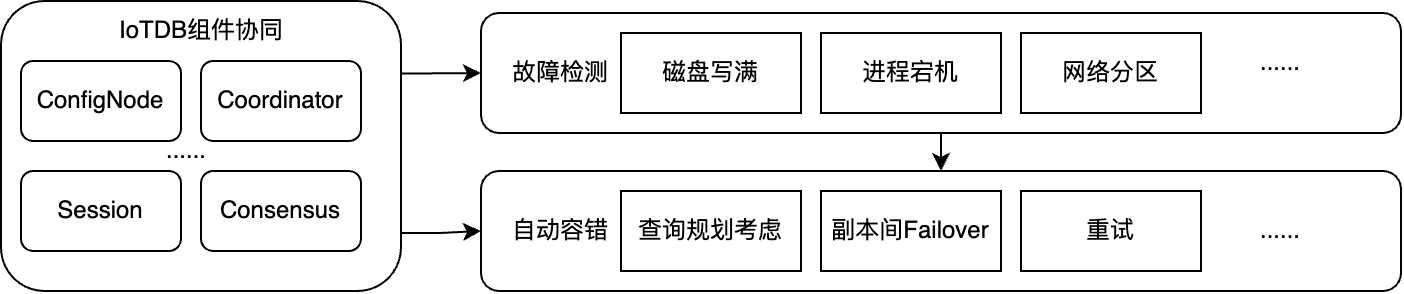
\includegraphics[width=0.99\linewidth]{1-overview-arch.png}
  \caption{IoTDB整体的高可用框架}
  \label{fig:c01-overview-arch}
\end{figure}

2. 将定义的高可用框架付诸实践,提高系统的故障检测和自动恢复能力。通过更加全面的故障检测,IoTDB能够更早、更准确地发现集群中发生的各种故障。在系统检测到故障之后,无需人工干预即可自动执行故障转移、节点替换、数据修复等操作,提升IoTDB分布式系统的韧性,使其能够应对更广泛的故障场景,减少人工干预的需求,并缩短故障恢复时间,从而保障系统的持续可用性,如图\ref{fig:c01-overview-arch}所示。

3. 对高可用架构和实现进行进行全面的测试与验证。本文将设计一系列覆盖各种故障场景的测试用例,包括模拟节点失效、网络分区、磁盘故障等。测试将关注系统的故障检测速度、恢复时间、数据一致性、以及对系统整体性能的影响等方面。通过严谨的实验和数据分析,我们将验证所构建的高可用性架构是否能够达到预期的目标。



\section{主要贡献}

本文的贡献主要体现在以下几个方面:

1. 提出了针对分布式系统故障场景和高可用架构的整体建模方法。本文研究了分布式系统中常见的故障种类,分析了故障的共性,并在此基础上提出了IoTDB高可用的整体方法论和架构。


2. 实现了高可用整体架构中的关键故障检测能力和自动容错和恢复能力。本文构建了更加完善的故障检测机制,并针对所有的故障建设自动容错能力,通过ConfigNode、客户端Session、服务端协调者、服务端共识模块等多个关键组件的协同,使得集群能够有效应对更广泛的故障类型,提升系统的韧性。


3. 进行了大量的测试和实验,证明了该高可用架构能够有效解决现有问题并应对新的挑战,为构建高可靠的分布式系统提供了实践支撑和数据验证。


\section{组织结构}
本文共分为8个章节,每个章节的内容如下:

第1章为引言部分,介绍了工业物联网、时间序列数据、时序数据库、Apache IoTDB、分布式数据库中的高可用性和容错能力等背景,阐述了本文建设更极致、更完善的可用性的研究动机,概括了本文的研究内容和研究贡献,描述了本文的组织结构。

第2章为相关研究综述,重点介绍了学术界对于分布式系统故障、高可用容错相关的研究,以及工业界多个广泛应用的分布式系统中的高可用方案的介绍。

第3章介绍了集群的故障检测和发现机制,包括基于ConfigNode Leader和DataNode之间心跳的节点存活探测、基于DataNode和DataNode之间心跳的集群拓扑探测、基于Phi Accrual算法的故障研判机制、基于集群监控的故障发现能力,和加速故障发现的若干优化。

第4章介绍了集群的故障恢复和容错能力,包括客户端、协调者、共识模块的三层联合容错机制。介绍了共识模块提供的数据副本容错基础,协调者模块利用多副本重试的容错尝试,客户端利用重试解决集群的暂时故障状态或不一致状态的能力,并阐述了故障时期的熔断和降级措施。

第5章介绍了集群对于经典故障场景的容错流程。结合第3章的故障检测和发现机制、第4章的故障恢复和容错机制,IoTDB集群能够抵御例如磁盘写满、进程宕机、网络对称/非对称分区、集群变更时的不一致等问题,并给出每种场景的详细容错流程。

第6章为实验部分。

第7章介绍了本文的工作总结和不足之处,并指出了未来工作的主要方向。
% !TeX root = ../thuthesis-example.tex

\chapter{相关研究综述}

\section{分布式系统故障}

从可能不可靠的部件构建可靠的系统是分布式系统的基本挑战。
分布式系统中的每个节点,无论是服务器、网络链路还是软件进程,都容易受到各种类型的故障的影响。这些组件的互连性意味着一个区域的故障通常会像滚雪球一样蔓延,导致更广泛的系统服务中断。

导致系统组件故障产生的原因众多,包括软件缺陷和硬件故障等,例如进程崩溃、磁盘损坏、程序错误会导致单一组件失效,网络延迟和分区可能导致系统组件的连接和通信出现故障,从而产生级联的连锁反应。系统组件故障的频率不容忽视。通常来讲,系统单一组件发生故障的时间间隔服从指数分布,多个组件之间的故障时间间隔相互独立,从而导致在大型分布式系统中故障的频率很高。根据谷歌的相关研究\cite{beyer2016site}, 每年会有超过1/100的机器出现内存崩溃,在百台节点组成的计算机集群,每一亿个小时会出现五千次左右的故障。

根据系统组件故障的产生原因,我们可以将分布式系统故障划分为以下几种类别\cite{michaud20062}:

1. 外部环境导致的故障。该故障产生的原因为不受控制的系统外部环境,例如机房停电、电缆断裂、火灾、地震海啸和其他自然灾害等。这种类型的故障无法通过分布式系统自身来自动解决和恢复,通常需要系统的搭建者通过在多个分散的地理位置部署数据和服务的副本来避免系统的中断和业务的损失。

2. 系统硬件失效导致的故障。该故障产生的原因为系统中一个或多个硬件不再正常工作,例如磁盘写满、内存不足、网络延迟等。这种类型的故障通常是高可用方案的重点解决对象,通过多副本、自动容错机制可以有效地减少这种故障对系统的实际影响。

3. 系统软件异常导致的故障。该故障产生的原因为应用程序在运行时出现偏离预期的行为,例如在缓冲区的边界之外写入数据导致内存损坏和进程崩溃、除零错误、返回值错误等。该问题通常不易解决,但是高可用方案可以为这类错误提供一定的容错和兜底。

4. 外部恶意攻击导致的故障。该故障产生的原因为人为恶意行为,例如例如代码注入攻击和ddos攻击等。该类故障通常通过专门的安全防御解决,但高可用方案方案依然可以在ddos等部分攻击场景下提供帮助,例如通过负载均衡的能力重新分配资源,从而让系统部分节点在遭受攻击和崩溃时依然能够提供服务。

本文提出的高可用方案的目标是“部分失效、整体可用”。具体而言,即使出于上述的任何原因系统内有部分组件出现故障,只要系统剩余存活的组件满足可用标准、资源足够、能够协同工作,那么系统就可以通过故障检测、自动容错、自动恢复等高可用机制保证服务的正常运行,降低错误在用户侧的感知,保证业务的连续性。

具体而言,本文提出的高可用方案能能够解决Kola\cite{kola2005faults}等人提出的分布式系统错误,包括以下具体问题:

1. 进程宕机,一些进程长时间甚至无限期地挂起,无法响应外部的请求。从请求方的角度来看,没有简单的方法来确定进程是否还在提供服务或是已经无法响应,

2. 磁盘空间不足。在数据暂存和写入期间,磁盘空间不足。

3. 硬件/软件/网络中断。间歇性网络中断、由服务器/客户端机器崩溃引起的中断以及用于硬件/软件升级和错误修复的停机时间导致在此期间的相关任务、RPC请求全部失效。

4. 资源过度消耗。由于并发数量过多、内存资源支出太多导致服务器崩溃,或是引发大量抖动导致传输效率降低、各种任务超时。


\section{高可用和容错}

\subsection{定义和衡量指标}

高可用性(High Availability)是分布式数据库系统的关键特性。
高可用性是指系统在正常状态和各种故障状态下保持运行和可访问的能力。高可用能力对于系统可靠性、数据完整性和业务连续性至关重要,有助于帮助客户减少服务中断,保持业务弹性,从而避免收入损失和声誉受损,帮助客户企业满足各种法规遵从性要求,满足客户的期望。

高可用性可以通过服务级别协议SLA(Service Level Agreements)和恢复时间目标RTO/恢复点目标RPO等指标进行衡量。
SLA的关键指标是服务的正常运行百分比,例如目标为“五个九”的可用性意味着系统在一年中的 99.999\% 的时间都应处于运行状态,每年的服务停止时间不超过0.0001\%(即53分钟)。RTO 是指从服务中断到恢复服务所需的最长可接受时间,而 RPO 是指在发生中断后可能丢失数据的最大可接受量时间。

容错能力(Fault Tolerance)是指系统在部分组件发生故障后仍能继续正确运行的能力,也是实现高可用性的关键方法。容错的目标通常是实现零停机时间,这通常通过基础设施中每个组件的备份或冗余来实现。


\subsection{常见的高可用容错机制}

高可用性和容错能力的架构模式关键在于消除单点故障(single point failure)、对系统故障进行检测、在冗余节点之间可靠地进行故障转移(failover)。

单点故障是指系统中一旦失效就会导致整个系统崩溃的任何组件。高可用性通过复制关键组件,如服务器进程、数据存储设备,在节点之间建立对等关系而不是依赖中央枢纽等方法来避免单点故障。
持续监控系统状态、检测系统故障并建立自动化故障转移机制对高可用性起到至关重要的作用。在故障发生后,自动化故障转移机制能够检测到故障,并自动将操作切换到备用组件,从而最大限度地减少停机时间。


数据复制(Replication)是消除单点故障的重要方法。数据复制是指在不同位置创建和维护相同数据或者服务的多个副本,以确保数据或服务可用性和可靠性。同步复制确保数据被写入所有副本后才返回结果,异步复制则优先考虑可用性和性能,允许数据首先写入主节点,然后再复制到其他副本,这可能会导致临时的数据不一致。数据副本因子(replication factor)决定了存储的数据副本数量。


共识协议(Consensus Protocol)在维护多份数据副本的一致性,使得分布式系统中的多个副本或机器对状态达成一致。根据副本拓扑结构,共识协议可以分成单一领导者、多领导者、无领导者结构。
根据数据一致性分类,共识协议可以分成线性一致性\cite{herlihy1990linearizability}、顺序一致性\cite{attiya1994sequential}、最终一致性\cite{bailis2013eventual}。最终一致性中可以继续细化为因果一致性\cite{lloyd2011cops}、会话一致性\cite{mortazavi2018session}、读己之写一致性\cite{nishtala2013memcached}。Paxos、Raft、ZAB、Gossip是著名的共识算法。
Paxos\cite{lamport2001paxos}基于无领导拓扑结构实现了线性一致性语义,协议由Proposer、Acceptor、Learner三种身份的节点共同完成,通过两阶段协议实现多副本共识,在工业界有广泛应用,例如Google Chubby\cite{burrows2006chubby}和Google Spanner\cite{corbett2013spanner},以及阿里巴巴的OceanBase\cite{zhen2014oceanbase}。
Raft\cite{ongaro2014raft}为单一领导者多追随者拓扑结构,提供了线性一致性语义。Raft通过大多数选举、状态机复制和日志一致性三个模块实现数据副本共识和安全性。Raft提出后被广泛运用在工业系统中,例如etcd\cite{etcd}和Apache Ratis\cite{ratis}。
ZAB\cite{junqueira2011zab}协议结构介于Paxos和Raft之间,由单一领导拓扑实现了强一致性。ZAB包含了Leader选举、数据发现、数据同步、全序原子广播四个阶段,是ZooKeeper\cite{hunt2010zookeeper}核心的一致性协议。
Gossip\cite{demers1987gossip}通过多副本无领导拓扑结构实现了最终一致性,由种子节点周期性选择邻居节点散步数据消息,最终同步给网络结构中的所有副本。节点往往采取last-writer-win算法来解决全局写入冲突。Gossip协议被运用在Apache Cassandra\cite{lakshman2010cassandra}和Consul\cite{mishra1993consul}等工业实现中。


故障转移和重试是常用的故障恢复方法。当系统中的主要副本发生故障或变得不可用时,系统自动或手动地将工作负载切换到其他副本上,通过在副本之间进行重试来确保服务的连续性和可用性。

故障转移机制的基础是故障检测和故障判定。
故障检测可以通过心跳机制进行健康检查,也可以依赖监控指标和日志进行人工分析,或者通过机器学习方法进行自动检测。故障判定可以基于规则算法(例如固定超时)、人工确认,或通过机器学习方法进行自动判断。
故障检测和判定的核心挑战在于在检测准确性和检测速度的两个维度上进行权衡。提高检测准确性通常意味着更低的误报率,代价是更慢的检测速度。而更快的检测速度往往意味着错报,触发不必要的故障转移。

故障转移机制的实现方法依赖在多副本之间重试。重试不但可以应对单一副本的非永久性的瞬时故障,例如网络抖动、短暂的资源过载等问题,也能通过将请求导引到其他副本上来应对单一副本的永久性故障,从而实现自动故障恢复,减少人工的干预和人力的投入。
根据不同的策略,重试可以分为立马重试、固定间隔等待重试、指数退避重试、随机退避重试和基于策略的重试方法。立马重试和固定间隔等待重试的实现简单,适用于预期故障能够快速恢复的场景,然而会给系统增加负载。
指数退避重试和随机退避重试是通过将每次重试之间等待的时间间隔设置成指数增长、增加随机抖动的方式缓解因频繁重试造成的系统压力,避免雪崩效应。基于策略的重试则需要请求的双方提前约定好不同的错误状态的含义和对应的重试策略,服务方根据对自身的状态评估给出一个错误状态交给请求方处理,提高重试的有效性。

故障恢复还包括对故障副本的自动修复。在数据库系统中,通常可以依赖消息日志(Message Logging)和检查点(Check-pointing)来实现。消息日志可以让系统记录所有关键操作或者状态变更,在系统出错之后依赖日志记录的顺序重新执行操作,即可完整恢复系统到故障前的状态。消息日志的现实应用场景包括数据库中的预写式日志(WAL)、Raft共识协议中的日志、分布式消息队列KafKa中的日志等。
检查点(Check-pointing)能够缩短故障恢复的时间。系统定期将其状态保存到可靠且稳定的存储介质上。崩溃后,系统从最后一个检查点重新启动并回放消息日志,而不是从头开始,大大缩短系统恢复时间。常见的检查点技术包括全量检查点、增量检查点和模糊检查点等,它们在性能和恢复速度上各有优劣。例如,LSM结构\cite{o1996lsmtree}的数据库会通过定期将内存中的MemTable刷盘形成SSTable,分布式计算框架Apache Spark\cite{zaharia2016spark}和Apache Flink\cite{carbone2015flink}也通过检查点技术来实现容错。


除了上述所言的反应式容错技术外,Ledmi\cite{ledmi2018fault}等人的研究还总结了主动式容错技术。
反应式容错(Reactive Fault Tolerance)指的是系统在发生故障之后采取措施进行恢复,而主动式容错(Proactive Fault Tolerance)指的是在系统发生故障之前就采取预防措施,预防故障的发生或减轻故障的影响。通常的步骤包括预测故障、预防故障、提前进行容错设计,核心思想是“防患于未然”。常见的主动式容错方案包含软件抗衰老(Software Rejuvenation)、预防式迁移(Preemptive Migration)、负载均衡(Load Balancing)等。

软件抗衰老通过定期或在特定条件下重启或刷新软件系统,以清除累积的错误状态和资源泄漏,从而防止系统崩溃或性能下降。系统在长时间运行过程中可能会积累内存泄漏、资源耗尽、线程死锁等问题,这些错误状态可能不会立即导致系统崩溃,但会逐渐降低系统的性能和稳定性。通过定期或在特定条件下重启或刷新系统,清除这些累积的错误状态,使系统恢复到健康状态。该技术在电信、航空航天、金融交易等系统中非常常见。

预防式迁移通常指预测到某个节点可能即将发生故障时,提前主动干预,服务或数据迁移到更安全或更稳定的节点上。这种预测通常基于系统的性能指标等内部状态信息、节点的负载信息和资源使用情况,或是在计划内的硬件维护、软件升级等之前。

负载均衡则通过将用户的请求或工作负载均匀地分配到多个服务器或组件上,从而主动避免单点故障。系统通常会部署多个能够提供服务的服务器,并通过将客户端的请求分发到多个服务器上,以平衡系统的负载,提高系统的整体性能和可用性,并允许服务增加服务器数量来实现系统的水平扩展,提高系统的容量和并发处理能力。在系统受到突发大流量压力的情况下,扩缩容配合负载均衡能够良好地扛住流量的压力,保障服务的平稳运行。



本文的高可用性和容错能力的建设主要集中在主动式容错机制的建设,即数据复制、共识协议、故障转移等方面。

本节的剩下部分将会对当代分布式系统中高可用性和容错性的实践展开研究。具体而言,本文会研究Cassandra、TiDB、Oceanbase三个成熟的分布式数据库系统的高可用和容错设计,作为后续IoTDB建设高可用性和容错能力借鉴和参考。



\section{Cassandra系统的高可用方案}
Cassandra\cite{lakshman2010cassandra}是一个开源的分布式NoSQL数据存储系统,用于管理分布在大量廉价服务器上的海量结构化数据,具备水平可扩展性、灵活的数据模型、没有单点故障的高可用性等优点。

\subsection{Cassandra系统整体架构}

\begin{figure}
  \centering
  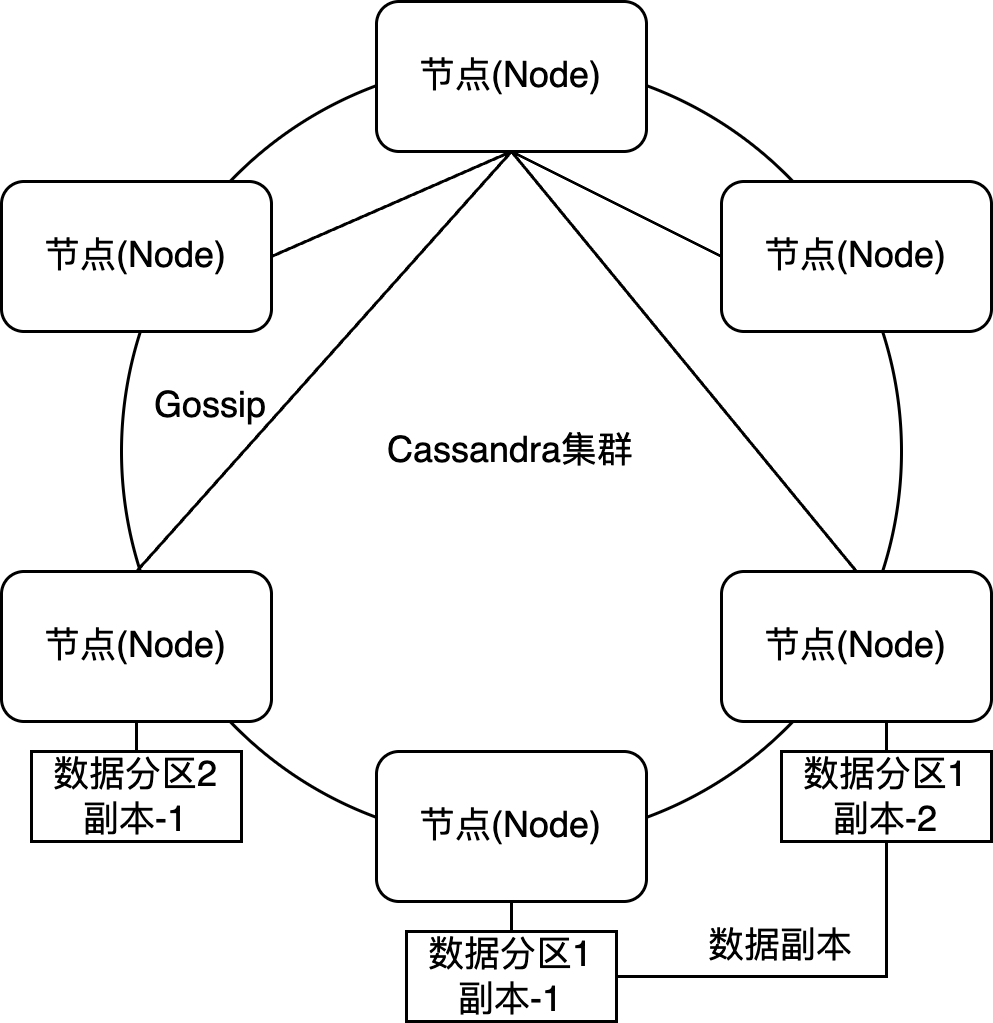
\includegraphics[width=0.5\linewidth]{cassandra-arch.png}
  \caption{Cassandra系统整体架构图}
  \label{fig:cassandra-arch}
\end{figure}

Cassandra基本组成单元是节点(Node),节点代表单个运行Cassandra进程的实例,通常运行在成本较低的商用硬件上。Cassandra集群中通常由多个节点组成。每个节点是同质性的,提供和其他节点完全相同的功能。
节点是Cassandra线性可扩展性的基础,通过增加节点进行横向扩展,Cassandra可以增加其管理的数据量、服务的吞吐量。
节点直接通过叫做Gossip的一种P2P协议进行通信。

Cassandra上管理的数据会被进一步划分为更小粒度的分区,从而在各个节点中均匀分布数据。Cassandra通过一致性哈希算法\cite{karger1997consistent}决定每个节点负责的数据范围。分区情况会被Gossip协议广播到所有节点,从而使每个节点都能够对外提供正确的服务。

Cassandra通过数据副本来保证可用性和容错能力,通过一致性协议保证副本的一致性。
Cassandra通过复制因子(RF)为同一个分区保留多个副本,保证即使一个副本宕机,其他副本仍然可以满足请求,且副本可以被放置在不同的数据中心,从而获得更高的安全性和性能。Cassandra通过一致性级别(CL)来决定操作的一致性,表示在操作被视为成功之前,必须向协调器确认读取或写入操作的最小Cassandra节点数。


\subsection{节点故障检测}

Cassandra中的每个节点通过Gossip协议来定期交换彼此的信息,并使用Phi累积性故障(Phi Accrual)检测算法\cite{hayashibara2004spl}来判断某个节点是否出现故障。

每个节点定期(通常每秒一次)通过Gossip协议选择几个节点交换彼此的状态信息,包括节点的运行状态、负载信息、该节点已知集群中其他节点的信息,使得信息可以快速有效地传播到整个集群。Gossip协议是一种最终一致性协议,随着时间的推移,所有节点最终都会收敛到一致的集群状态。

Cassandra的Phi累积性故障检测算法会根据Gossip交换的状态信息来计算出某个节点失效的可能性,避免了简单的地使用超时机制,而是通过统计分析心跳间隔,来预测节点失效的概率。Phi Accrual检测器会记录节点之间心跳信息到达的时间间隔,计算出一个“Phi”值,表示节点失效的可能性。Cassandra会设置一个Phi阈值,当Phi值超过这个阈值时,就认为节点失效。Phi Accrual检测器能够根据网络状况动态调整在网络不稳定的情况下,它会降低Phi阈值,以避免误判,在网络稳定的情况下,它会提高Phi阈值,以提高检测的准确性。在瞬态网络问题期间,节点可能暂时无法访问。使用phi accrual可以更宽容的对待这类网络问题,减少不必要的节点失效判断。


\section{TiDB系统的高可用方案}
TiDB\cite{huang2020tidb}是开源的分布式关系性数据库,同时支持OLTP和OLAP的能力,具备水平扩缩容、金融级高可用、实时 HTAP、云原生、兼容MySQL生态等优势。

\subsection{TiDB的整体架构}

TiDB集群可以划分为位于中间代理层的TiProxy,位于计算层的TiDB,和位于存储层的TiKV和TiFlash,以及集群的协调节点PD(Placement Driver)。

\begin{figure}
  \centering
  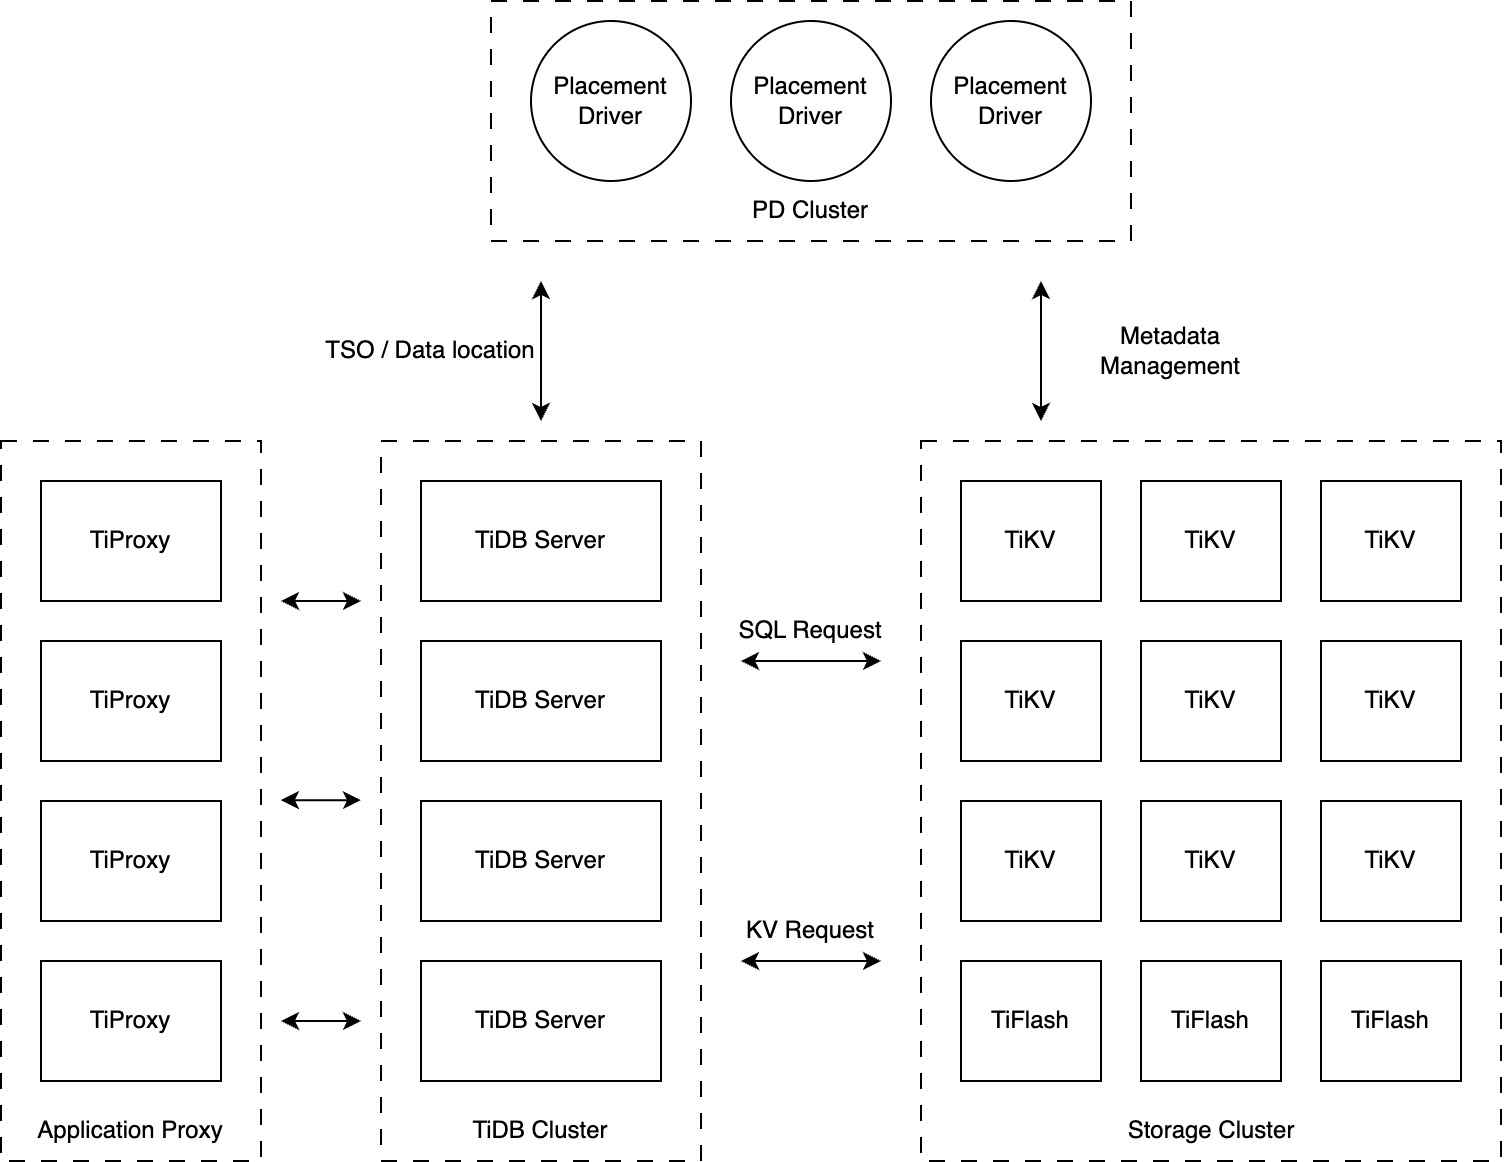
\includegraphics[width=0.9\linewidth]{tidb-arch.png}
  \caption{TiDB系统整体架构图}
  \label{fig:tidb-arch}
\end{figure}

PD(Placement Driver)是集群的大脑,负责元信息管理,实时监控和调整集群节点的整体拓扑结构、每一个节点的数据分布情况。

TiKV和TiFlash是数据的存储节点。TiKV是具备分布式事务能力的键值存储引擎,而TiFlash是为查询负载专门优化的列式存储引擎。
数据的存储以Region作为单位,包含了一段Key的区间,TiKV通过Region来实现数据分区和负载均衡,并会为每一个Region维护多个副本来服务高可用性。

TiDB是无状态的计算节点,负责接受客户端的连接,对SQL解析和优化,生成分布式执行计划,并将计划转发给存储节点进行执行。

TiProxy是部署在客户端应用和TiDB之间代理节点,提供负载均衡、连接持久化、服务发现和其他功能。


\subsection{故障的检测和发现}

在TiDB集群中,PD负责检测定期交换心跳来维持对每个节点、每个Region和集群全体的拓扑的拓扑感知,并会在检测到错误的时候尝试自动恢复。TiDB Server会通过PD获取最新的数据分区和地址,生成对应的查询计划。TiProxy会保持对TiDB Server的检测和探活。

TiKV会定期向PD发送心跳包,交换的内容包括总磁盘容量和磁盘用量、节点承载的Region数量、数据写入和读取的负载情况、发送/接受的snapshot数量等相关信息。如果PD在一段时间内没有收到TiKV的心跳,那么就会认为该节点可能出现故障,将其状态标记为异常,并且综合考虑用户配置和集群实际情况,来判断是否将该节点从集群中移除,并进行相应的调度操作,例如将该TiKV上的Region进行迁移。

每一个Region的Raft Leader也会定期向PD发送心跳包,交换的内容包括Leader所在的位置、每一个Follower所在的位置、掉线的副本个数和该Region的写入/读取速度。当Leader掉线,其他的Follower节点可能会触发新的选举,同时若PD长时间没有收到心跳,也可能触发主动的Leader切换和副本的调度。

\subsection{最高级别的容灾能力}

通过多数据副本、多机房部署、多地分布部署,TiDB集群可以实现RPO为零,RTO在一分钟以内的目标,同时容忍单节点故障、数据中心故障、一整个城市级别的灾难。以下是对TiDB的两地三中心五副本的部署结构描述:




\section{Oceanbase系统的高可用方案}

Oceanbase是开源的分布式关系性数据库,兼具分布式架构的扩展性和集中式架构的性能优势,过单一引擎支持混合事务/分析处理(HTAP),具备强数据一致性、高可用性、高性能、在线扩展、与 SQL 和主流关系型数据库的高度兼容性等优势。

\subsection{Oceanbase的整体架构}

Oceanbase集群主要包括OBServer和OBProxy两个角色。每一个OBServer上都运行着Oceanbase的一个进程,内部可进一步细分为根服务(Root Service)、SQL引擎、事务引擎和存储引擎。OBProxy则充当中间层,接收来自应用程序的SQL请求将其路由到集群内最佳的OBServer节点,然后将执行结果返回给应用程序。

\begin{figure}
  \centering
  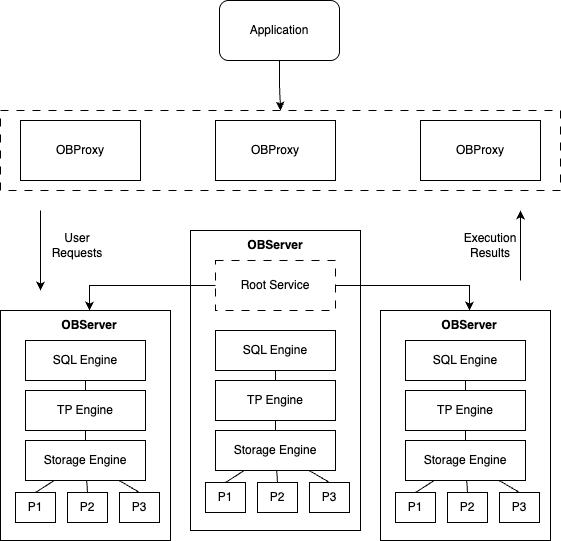
\includegraphics[width=0.9\linewidth]{oceanbase-arch.png}
  \caption{Oceanbase系统整体架构图}
  \label{fig:oceanbase-arch}
\end{figure}

根服务是集成在Oceanbase进程内的逻辑服务,负责维护集群的元数据,包括表结构、分区信息、节点状态等。根服务会通过心跳机制检测每一个OBServer的健康状况,如果发现故障,则会触发恢复流程,包括重新选举领导者或重新复制分区。根服务还会负责监控集群的负载情况,会进行分区移动、分区复制和领导者切换等操作,以确保各个节点的资源利用率均衡。

OBServer还包含了SQL引擎,用于接受用户请求并生成对应的计划,以及基于LSM结构的存储引擎。

集群内的元数据和用户数据都是以分区的方式进行水平划分和存储,并通过副本复制的方式保证分区的高可用。Oceanbase采用了基于哈希和范围的双层划分算法,但会保证同一个表组的分区被分配在同一个节点上。Oceanbase采用Paxos对每一个分区的redo log进行复制管理,在故障恢复的时候,通过重放redo log实现恢复。

OBProxy 用于将请求路由到 OBServer。当接收到用户的 SQL 查询时,OBProxy 将解析该查询,然后根据分区的位置信息将查询发送到相应的 OBServer,提供服务发现和负载均衡等能力。


\subsection{Oceanbase的快速故障发现}

OceanBase通过校验和、针对Paxos恢复和选举优化、基于RPC机制的节点检测等方式尽可能提前错误发生的时间。

在校验和上,Oceanbase在每次从磁盘中读写数据的时候都会计算和比较校验和,在每次大合并之后对每一个数据分区的副本重新比对校验和,在重放Redo Log的时候会计算每一条事务的累积校验和。通过事务粒度的校验和机制,Oceanbase能够发现软件实现中事务处理和并发控制两个模块的人为程序漏洞。

在Paxos算法上,Oceanbase通过大幅减少故障单元和稳定的选举算法来提高故障的发现能力。
在前文所提到的TiDB中,故障恢复单元是每一个Raft组。当上层业务的分区特别多、单一节点上承载的Raft数量特别多的情况下,故障恢复的单元数量就会水平扩张,量级巨大。然而,在Oceanbase 4.0版本之后,故障恢复的单元转变成一个单机的日志流,在逻辑上可以把每一个节点视作一个整体的Paxos组,因此故障恢复单元将不再和业务的元数据和实际数据量有关,从而进一步降低了故障恢复的复杂性和时间。
传统的Paxos选举流程基于随机算法,并且依赖节点之间的时钟同步,例如NTP。Oceanbase的实现消除了对节点间时钟同步的依赖,完全基于消息驱动,依靠节点之间的消息交互和顺序来触发选举,并激进地将Leader的Lease时间缩短到了4s以内,从而能够更快地检测到故障并完成新的Leader选举。

Oceanbase 4.0中,节点间健康状态监测机制从基于TCP的连接机制转变为基于RPC框架内部的方式。3.0版本中OceanBase采用定期发送TCP Keepalive的探测包来检测节点之间的网络连接是否正常,然而这种检测只能用于判断网络情况,如果OBServer进程出现问题(例如Coredump崩溃),但TCP连接依然存在,KeepAlive机制无法识别。因此,在4.0版本中,Oceanbase框架内值了健康状态监测机制,通过定期发送应用程序级别的心跳包,从而能同时监测网络和进程的健康。同时,由于RPC 框架内部的检测机制能够检测应用程序的响应延迟、错误率等指标,从而提供更细粒度的健康状态信息。

\subsection{Oceanbase的故障恢复和Client协同}

Oceanbase通过Paxos并行回放、故障时期领导指定、Client的建连探活等方式提高故障恢复的速度。

在前一节所述,Oceanbase的故障恢复单元是一个单一的Paxos Group,为了提高故障恢复的速度,Oceanbase需要进行并行、实时地回放日志中的事务,从而防止日志回放成为性能的瓶颈。在Oceanbase中,不同事务的Redo日志可以并行回放,同一事物的不同Redo日志也可以并行回放,通过事务的ID




\section{表格}

表应具有自明性。为使表格简洁易读,尽可能采用三线表,如表~\ref{tab:three-line}。
三条线可以使用 \pkg{booktabs} 宏包提供的命令生成。

\begin{table}
  \centering
  \caption{三线表示例}
  \begin{tabular}{ll}
    \toprule
    文件名          & 描述                         \\
    \midrule
    thuthesis.dtx   & 模板的源文件,包括文档和注释 \\
    thuthesis.cls   & 模板文件                     \\
    thuthesis-*.bst & BibTeX 参考文献表样式文件    \\
    \bottomrule
  \end{tabular}
  \label{tab:three-line}
\end{table}

表格如果有附注,尤其是需要在表格中进行标注时,可以使用 \pkg{threeparttable} 宏包。
研究生要求使用英文小写字母 a、b、c……顺序编号,本科生使用圈码 ①、②、③……编号。

\begin{table}
  \centering
  \begin{threeparttable}[c]
    \caption{带附注的表格示例}
    \label{tab:three-part-table}
    \begin{tabular}{ll}
      \toprule
      文件名                 & 描述                         \\
      \midrule
      thuthesis.dtx\tnote{a} & 模板的源文件,包括文档和注释 \\
      thuthesis.cls\tnote{b} & 模板文件                     \\
      thuthesis-*.bst        & BibTeX 参考文献表样式文件    \\
      \bottomrule
    \end{tabular}
    \begin{tablenotes}
      \item [a] 可以通过 xelatex 编译生成模板的使用说明文档;
        使用 xetex 编译 \file{thuthesis.ins} 时则会从 \file{.dtx} 中去除掉文档和注释,得到精简的 \file{.cls} 文件。
      \item [b] 更新模板时,一定要记得编译生成 \file{.cls} 文件,否则编译论文时载入的依然是旧版的模板。
    \end{tablenotes}
  \end{threeparttable}
\end{table}

如某个表需要转页接排,可以使用 \pkg{longtable} 宏包,需要在随后的各页上重复表的编号。
编号后跟表题(可省略)和“(续)”,置于表上方。续表均应重复表头。

\begin{longtable}{cccc}
    \caption{跨页长表格的表题}
    \label{tab:longtable} \\
    \toprule
    表头 1 & 表头 2 & 表头 3 & 表头 4 \\
    \midrule
  \endfirsthead
    \caption*{续表~\thetable\quad 跨页长表格的表题} \\
    \toprule
    表头 1 & 表头 2 & 表头 3 & 表头 4 \\
    \midrule
  \endhead
    \bottomrule
  \endfoot
  Row 1  & & & \\
  Row 2  & & & \\
  Row 3  & & & \\
  Row 4  & & & \\
  Row 5  & & & \\
  Row 6  & & & \\
  Row 7  & & & \\
  Row 8  & & & \\
  Row 9  & & & \\
  Row 10 & & & \\
\end{longtable}


\chapter{数据复制和共识协议}

数据复制和共识模块是构建高可用和容错能力强大的分布式系统的基石。
在Apache IoTDB中,数据复制和共识协议由共识模块实现。
本节将会介绍IoTDB的共识模块,阐述IoTDB的统一共识模块的设计考量,详细介绍三个不同一致性级别的共识算法实现:RatisConsensus,IoTConsensus和IoTConsensusV2,并且给出每一个共识算法的可用性保障语义。


\section{共识模块概述}

在Apache IoTDB中,共识模块是构建高可用能力和故障容错能力的基石。IoTDB的所有核心功能,无论是用户数据的管理,还是集群元数据的维护,乃至负责全局服务配置和协调的ConfigNode服务,都依赖共识模块提供的能力。

共识模块的核心目标在于为同一份数据维护多个满足一致性要求的数据副本。这种数据副本的能力是是抵御单点故障、实现自动容错能力的直接基础,也是负载均衡、节点扩缩容等高级功能的前提。
从自动容错的角度来看,当某个存储数据的节点发生宕机或网络不可达时,系统可以依赖其他副本上的数据继续对外提供服务,从而避免了数据丢失和服务中断。
从负载均衡和扩缩容的角度来看,应用可以选择将读请求分散到不同的副本上,有效提升系统的并发处理能力;在需要进行节点维护或集群规模调整时,共识协议负责在节点之间实现副本数据的搬运,保证数据不丢失的前提下安全地迁移数据和调整节点数量。

在对内的实现上,共识模块隐藏了数据副本同步和一致性维护过程中所面临的诸多复杂挑战,包括但不限于高效地进行数据的同步/异步复制,如何保障每一个副本在故障情况下都能在最终状态上保持高度一致,如何在网络波动下的实现数据的断点续传,如何处理并发写入时可能出现的数据冲突并根据预设的解决策略确保一致性等内容。

对外而言,共识模块的抽象极大地简化了上层依赖模块的开发工作。
对于数据写入模块而言,它不需要关心底层数据是如何同步到多个副本的,只需要向任何一个副本的共识模块提交写入请求即可,共识模块保证了请求返回时数据已经达到一致性级别的复制。这种简化降低了写入模块的复杂性,使其可以更专注于业务逻辑的实现。
对于数据查询模块来说,查询引擎可以放心地从任意一个可用的副本读取数据,并能够确保读取到的数据满足系统所定义的一致性级别。
这种设计上的解耦不仅降低了开发难度,也提升了系统的整体可维护性和可扩展性。


\section{共识模块统一框架}

IoTDB内部的不同应用模块需要依赖不同级别的共识协议,这种需求驱动了IoTDB建立统一的共识模块框架,通过可配置可插拔的共识协议来满足不同应用模块的需求,并为系统未来集成新的共识协议提供了扩展性。

\begin{figure}
    \centering
    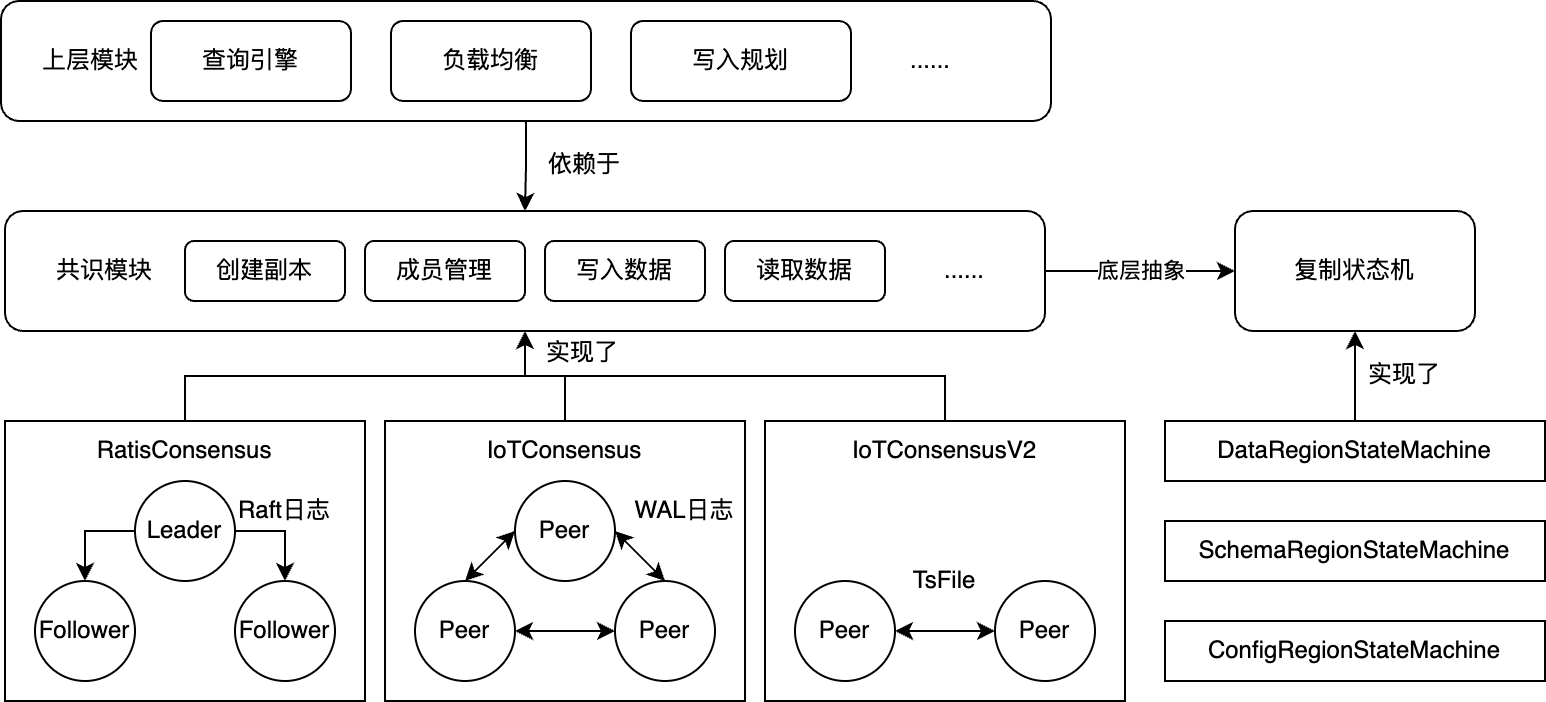
\includegraphics[width=0.99\linewidth]{c04-consensus-arch.png}
    \caption{共识层统一框架架构图}
    \label{fig:c04-consensus-arch}
  \end{figure}
  
图\ref{fig:c04-consensus-arch} 给出了共识模块统一框架的示意图。

共识模块要求所有的上层服务遵循复制状态机(replicated state machine)\cite{lamport1978statemachine}的规范。目前,实现了复制状态机规范的包括了存储引擎DataRegionStateMachie,元数据存储引擎SchemaRegionStateMachine和集群分区和管理服务ConfigRegionStateMachine。

共识模块定义了针对数据副本组的标准接口,包括创建和销毁数据副本、在数据副本上执行写入操作、从数据副本中读取数据、对数据副本的数量、组成成员进行变更等能力。

目前IoTDB中实现了共识模块标准接口的共识协议有三种,分别是基于Raft算法的强一致性共识协议RatisConsensus,基于多主复制的会话一致性共识协议IoTConsensus和基于主从快照同步的最终一致性共识协议IoTConsensusV2。

本章节的剩下部分会介绍每一种共识协议的实现细节。


\section{RatisConsensus}

RatisConsensus是IoTDB提供的强一致性共识协议实现,基于Raft共识算法和Apache Ratis\cite{ratis}开源项目实现。由于RatisConsensus给出了强一致性的语义保障,目前已成为集群元数据管理和ConfigNode分区服务默认的共识协议。

RatisConsenus内部会维护奇数(2n+1,默认为3)个副本,并为每一个副本提供强一致性的语义保障。由于底层依赖的Raft算法是基于单主复制结构的共识协议,因此在任何时刻,这些副本只有一个可以接受上层的写入请求,被称为Leader副本,剩下节点从Leader副本同步数据,可以接受只读请求。
RatisConsensus能够自动容忍少数副本的失效依然保持数据和服务的可用性。具体来说,对于一个2n+1副本的RatisConsensus服务,最多能够容忍n个副本的失效。同时,RatisConsensus能够保证在网络分区情况下的数据一致性,同一时刻能保证最多只有一个副本成为Leader副本。
当Leader副本失效之后,RatisConsensus内部存在自动故障转移的机制,通过新一轮的内部选举在短时间内(默认4-8秒)选出一个新的Leader副本。

RatisConsensus底层的一致性协议是Raft算法,包含Leader选举、日志复制和安全性保障等核心要素。Raft通过随机超时来实现Leader选举,通过任期(Term)来保证每次选举的唯一性和权威性。Leader接受写入数据,并将自身日志强制复制给所有Follower,最终所有的日志可以被排列出一个副本之间达成共识的全序序列,不同的副本均按照这个全序序列应用日志,从而实现副本数据之间的一致性。为了确保安全性,Raft 引入了 Commit 机制,即只有在大多数副本上保存了对应日志条目后,该日志才能被 Commit,上层才能收到共识层写入成功的回应。

\begin{figure}
  \centering
  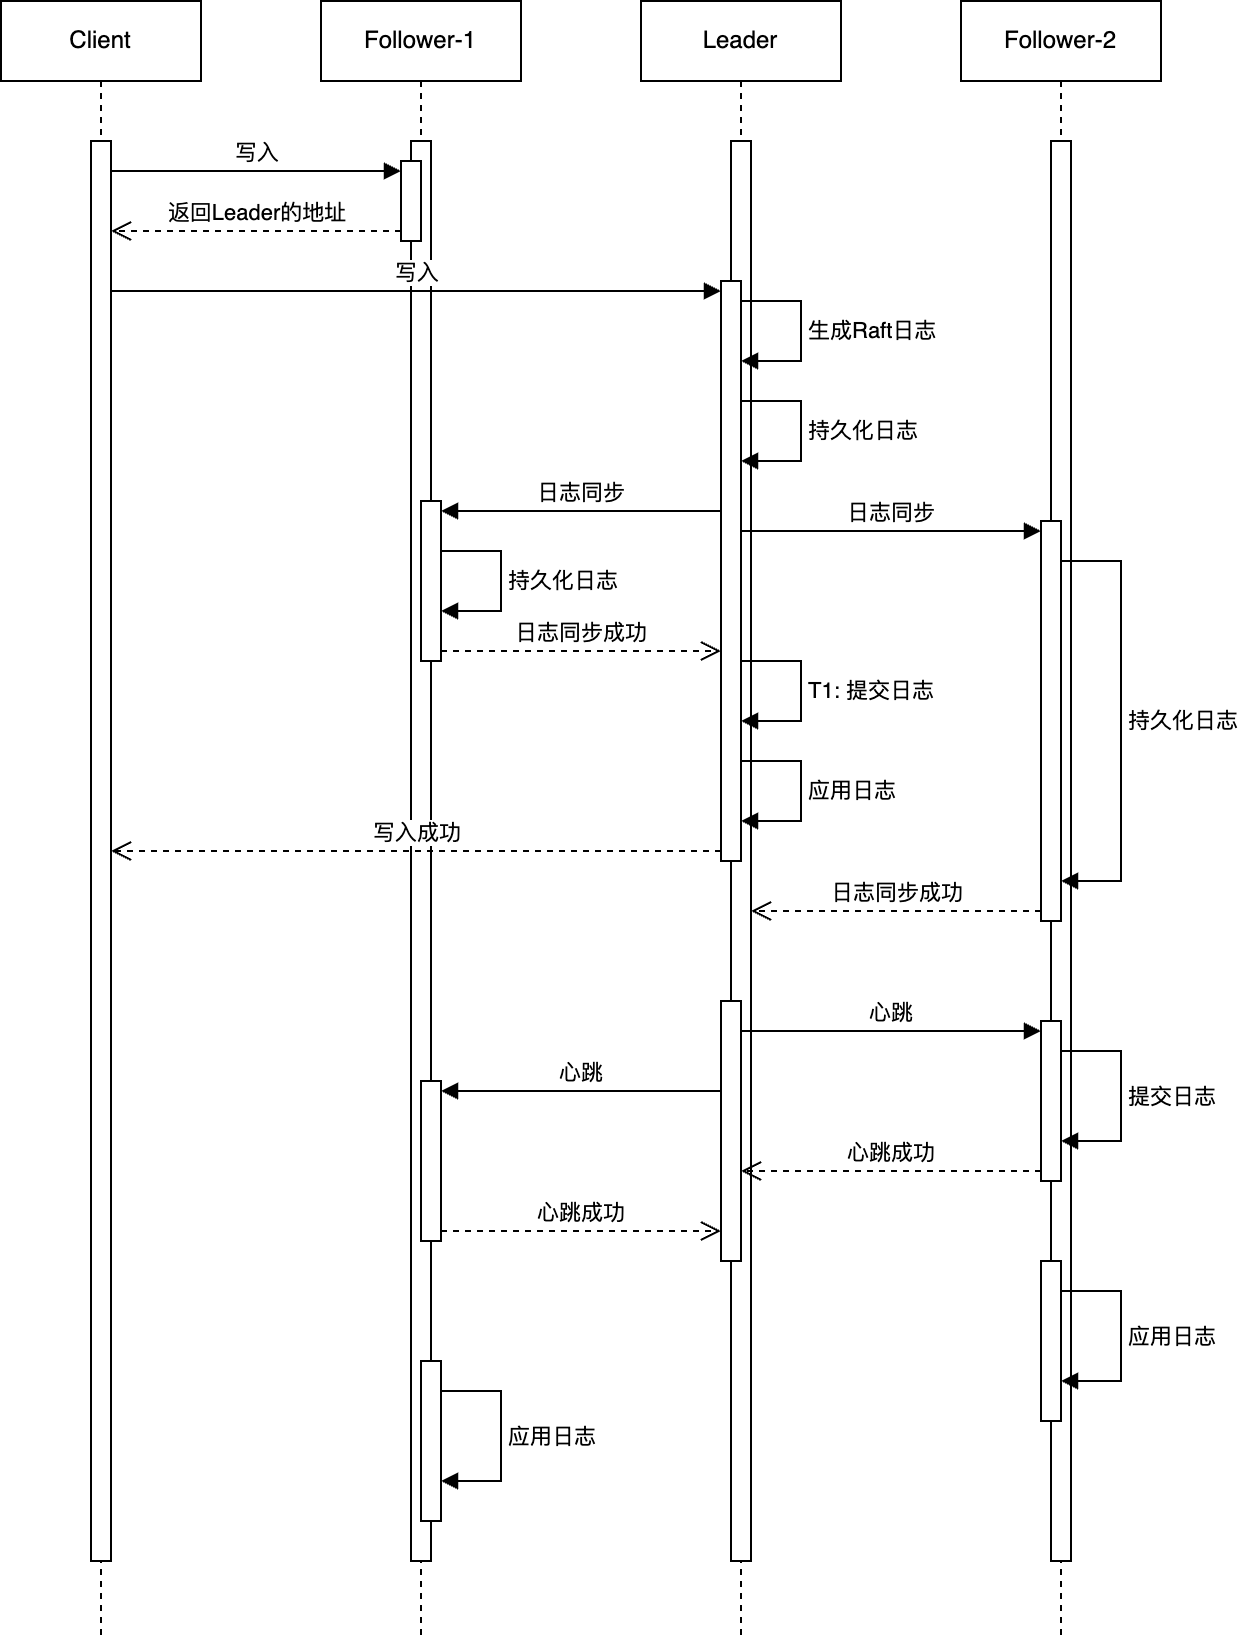
\includegraphics[width=0.7\linewidth]{c04-ratis-write.drawio.png}
  \caption{RatisConsensus数据写入和副本复制流程}
  \label{fig:c04-ratis-write}
\end{figure}

图\ref{fig:c04-ratis-write}给出了一条数据提交给RatisConsensus之后背后的数据复制流程。用户写入数据之后,会由Leader这边负责生成持久化日志并同步到所有节点上,在T1时刻,有超过半数的节点完成持久化同步之后,该操作的状态将会改变成Commit,Leader会应用这个日志并返回对应的结果。Raft算法会在后台保证所有节点能够最终都Commit并应用这个日志。



\section{IoTConsensus}

IoTConsensus是IoTDB提供的会话一致性共识协议实现,基于多主异步复制的自研实现,针对工业物联网时序场景写入模式有针对性的优化。目前,IoTConsensus是集群数据管理的可选共识协议之一。

IoTConsensus的设计初衷是为牺牲一定的可用性换取极致的可用性和更高的性能。
用于在工业物联网场景中,设备不断的时序数据,每台设备的写入请求往
往是串行无重复的,因而并发的写入请求之间通常不存在冲突。因此,IoTConsensus放宽了串形化的一致性约束,允许任何一个副本都能接受读写请求,并且请求在一个副本上执行成功即可返回客户端操作成功。


\begin{figure}
  \centering
  \subcaptionbox{IoTConsensu整体结构\label{fig:c04-iot-arch}}
    {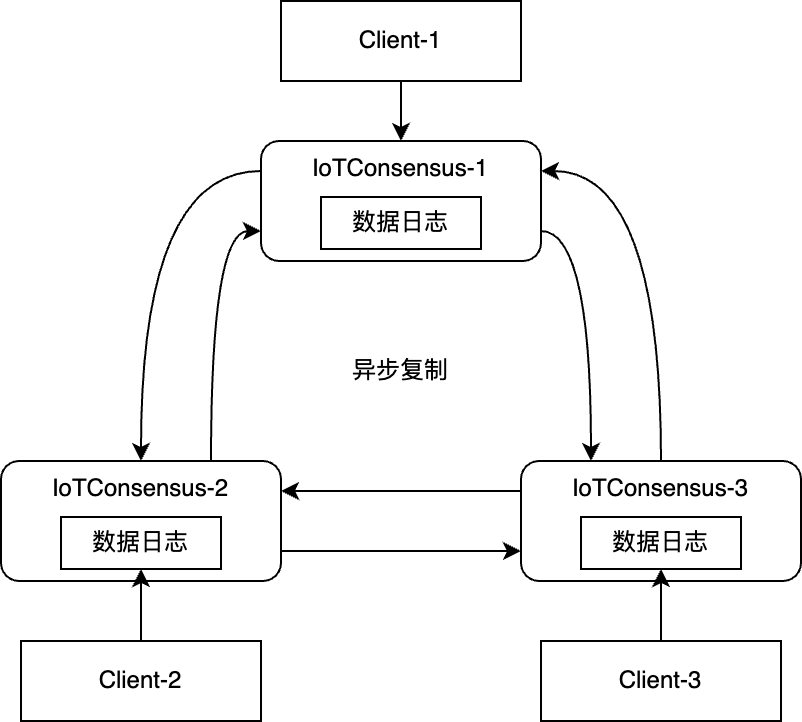
\includegraphics[width=0.4\linewidth]{c04-iot-arch.png}}
  \subcaptionbox{IoTConsensus写入流程\label{fig:c04-iot-write}}
    {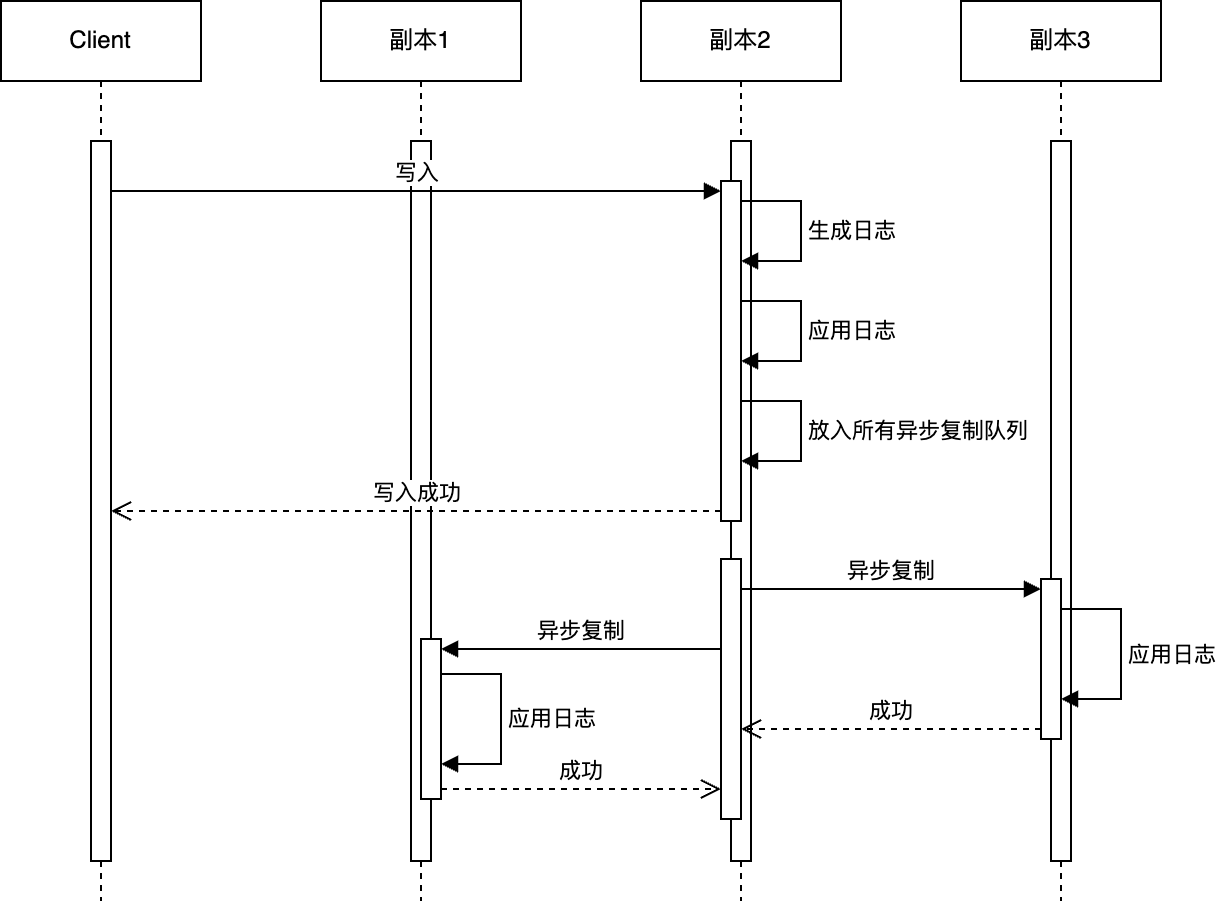
\includegraphics[width=0.58\linewidth]{c04-iot-write.png}}
  \caption{IoTConsensus示意图}
  \label{fig:c04-iot-consensus}
\end{figure}

图\ref{fig:c04-iot-arch}展示了IoTConsensus的结构,允许任何一个副本接受客户端的写入请求,并通过每个节点的后台异步复制线程将写入请求通过WAL的方式同步给其他的副本。


值得注意的是,当不同副本的数据产生冲突是,可能会导致副本之间数据无法达到最终一致,该问题的解决需要应用层的介入。例如在 Apache IoTDB 中,如果观察到某个序列的数据在不同副本上不一致,则可以使用 Select Into 子句拉取该序列在当前 Leader 副本上的数据并
重新向该共识组流式写入。但在绝大部分的正常应用场景,这种不一致不会发生。

虽然IoTConsensus支持多个副本的同时并发写入,但在实践过程中,为了提高性能、降低并发冲突,ConfigNode会为IoTConsensus挑选一个名义意义上的“主副本”,并默认将所有的写入请求引导到这个请求上。当“主副本”发生故障时,ConfigNode会启动故障容错和恢复机制,推举一个新的副本成为名义“主副本”。


\section{IoTConsensusV2}

IoTConsensusV2是IoTDB提供的最终一致性共识协议实现,基于主从异步复制的自研实现,针对工业物联网时序场景写入模式有针对性的优化。目前,IoTConsensusV2是集群数据管理的可选共识协议之一。

IoTConsensusV2相较于IoTConsensus相比,进一步牺牲了副本之间的同步时延、一致性级别,换取了极高的写入吞吐。IoTConsensusV2的总体思路是允许在部分场景下使用TsFile进行副本间的数据同步。基于TsFile的同步过程仅涉及到常数级别的复杂度操作,同时不用经过 WAL 的磁盘持久化和 Memtable 的内存维护,因此写入吞吐非常高,并且能够解决IoTConsensus存在的由于Follower宕机或Leader节点写入速率大于同步速率导致的WAL文件堆积和写入阻塞的问题。

然而,TsFile的生成相比每一条写入日志需要较长的时间,副本间数据同步延迟在极端环境下可达到几十分钟甚至是几个小时的数据。在两副本的情况下,如果主副本宕机,可能出现由于部分数据还未同步导致的数据暂时丢失的情况。如果宕机节点后续永久没有加入集群,那么这部分数据就会永久丢失。

\begin{figure}
    \centering
    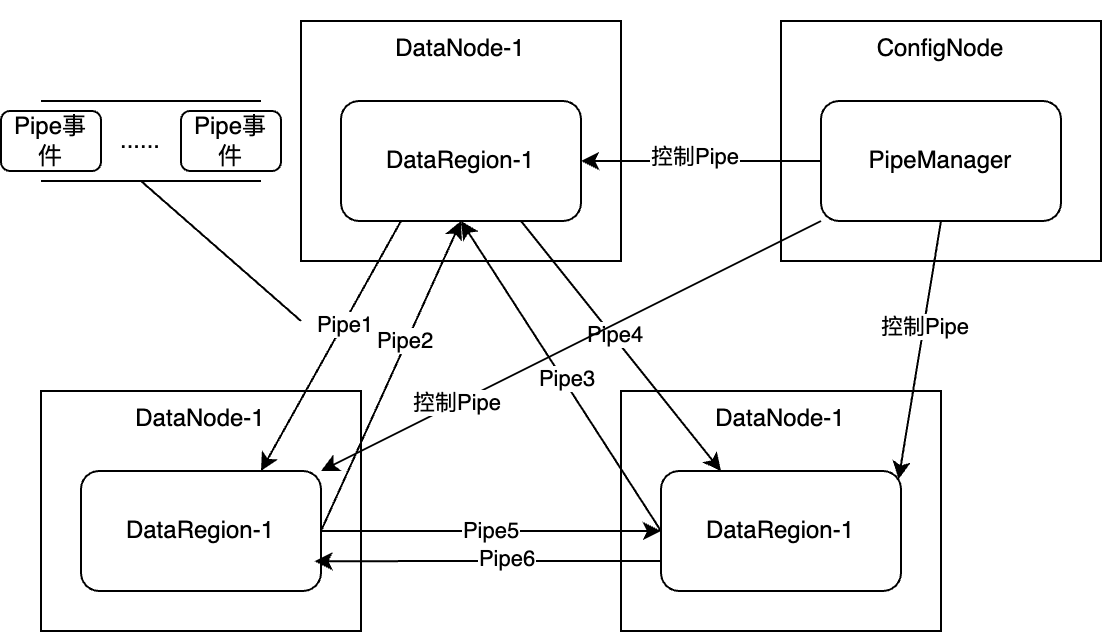
\includegraphics[width=0.8\linewidth]{c04-pipe-consensus.png}
    \caption{IoTConsensusV2的整体结构}
    \label{fig:c04-pipe-consensus}
  \end{figure}
  
图\ref{fig:c04-pipe-consensus}给出了IoTConsensusV2的整体架构。IoTConsensusV2具备以下两种同步模式:

1. Stream传输模式。在默认状态下使用WAL进行数据同步,来达到更快的同步速度和更高的一致性。当WAL堆积或者TsFile堆积的场景下,切换到TsFile进行数据传输,来达到更低的资源消耗和更高的吞吐。

2. Batch传输模式。该模式下,所有的数据同步都通过TsFile实现。

和IoTConsensus相似,ConfigNode也会为IoTConsensusV2挑选一个名义意义上的“主副本”,并默认将所有的写入请求引导到这个请求上。当“主副本”发生故障时,ConfigNode会启动故障容错和恢复机制,推举一个新的副本成为名义“主副本”。


\section{共识模块总结}

下表给出了共识模块三个共识协议的对比。

\begin{table}
    \centering
    \caption{共识协议对比}
    \begin{tabular}{cccc}
      \toprule
      特性         & RatisConsensus & IoTConsensus &  IoTConsensusV2 \\
      \midrule
      副本一致性级别   & 线性一致性 & 会话一致性 &  最终一致性 \\
       副本复制策略    & 半同步    & 异步       & 异步       \\
       自动故障转移    &  内部选举    &   ConfigNode指定    &  ConfigNode指定  \\ 
      共识协议结构   & 主从 & 多主 &  多主  \\
      数据同步性能   & 一般 & 较高 &  极高  \\
      \bottomrule
    \end{tabular}
    \label{tab:consensus-compare}
  \end{table}




% !TeX root = ../thuthesis-example.tex

\chapter{集群故障检测和判断}

集群故障检测和判断是构建高可用自动容错能力的先决条件。如同医生诊断病情是进行治疗的第一步,系统也必须先感知到问题的存在,才能采取相应的应对措施。及时、准确地识别出集群中发生的各种故障,是后续所有容错机制得以有效运行的前提。

本章节描述了高可用框架下的集群故障检测和判断机制。管理节点是集群的大脑,负责集群故障检测和研判。管理节点通过和集群所有成员交换心跳定期收集信息,并使用集群故障研判的算法来发现故障。

本节描述了管理节点、数据节点和客户端之间通过心跳探知其他节点状态的机制,并描述了基于心跳历史的固定超时、Phi Accrual算法的故障研判机制。


\section{不同角色的状态感知机制}

\subsection{管理节点感知其他节点状态}

管理节点节点通过共识心跳感知其他管理节点的状态,通过定期的心跳RPC感知所有数据节点的状态。

管理节点 集群通过 Raft 协议中领导者定期发送的心跳以及 Follower 基于这些心跳维护的选举超时计时器,实现了对集群中其他管理节点的成员列表、每个成员的基本存活状态的高效感知。一旦心跳机制指示领导者节点失联或故障,就会触发 Raft 的选举流程,确保管理节点集群在面对节点失效时能够及时地重新组织并恢复正常工作。

IoTDB通过管理节点和数据节点定期交换心跳的机制来维护每一个数据节点节点的信息,并用这些信息进行磁盘、进程和对称网络分区的故障探测。管理节点和数据节点之间心跳交换的具体实现如下。

管理节点会将集群的所有数据节点纳入心跳管理的范畴。具体来说,数据节点在启动时都需要向管理节点的领导者节点汇报和注册自己。一经注册,管理节点领导者就会将这个进程纳入到心跳管理的范围内。同样,在节点下线维护、被移出集群、重启时也会向管理节点进行汇报,由管理节点决定是否要将节点移除出心跳管理的范畴。

对于纳入心跳管理范畴的节点,管理节点会按照固定时间间隔(默认为1s)向这些节点的内部端口发送RPC心跳探测,并要求节点上传自身的信息,确认最新的状态。以数据节点为例,数据节点需要通过心跳上报当前的存活状态、节点的CPU负载率、内存占用率、磁盘的消耗情况以及数据节点上每一个分区的情况,包括分区领导者的身份确认、每一个分区的磁盘占用情况、副本日志同步的情况、数据节点上所有pipe任务的情况。

通过定期交换信息,管理节点能够掌握节点的全局信息,并利用上述这些信息展开对磁盘写满、节点宕机、网络对称分区等错误的检测。具体的检测方法可以参考后续的章节\ref{failure_detection}。

\subsection{数据节点感知其他节点状态}\label{sec:数据节点-intra-heartbeat}

通过和管理节点交换心跳,数据节点能够实时感知管理节点的列表和存活状态。

为了让数据节点能够实时感知其他数据节点成员的状态,本文提出基于数据节点间的对等心跳汇总的集群拓扑感知机制,通过数据节点之间定期交换心跳来获取相互之间的连通性,并将所有节点的结果汇总上报给管理节点领导者,从而使管理节点领导者具备集群的网络拓扑感知能力。

\begin{figure}
  \centering
  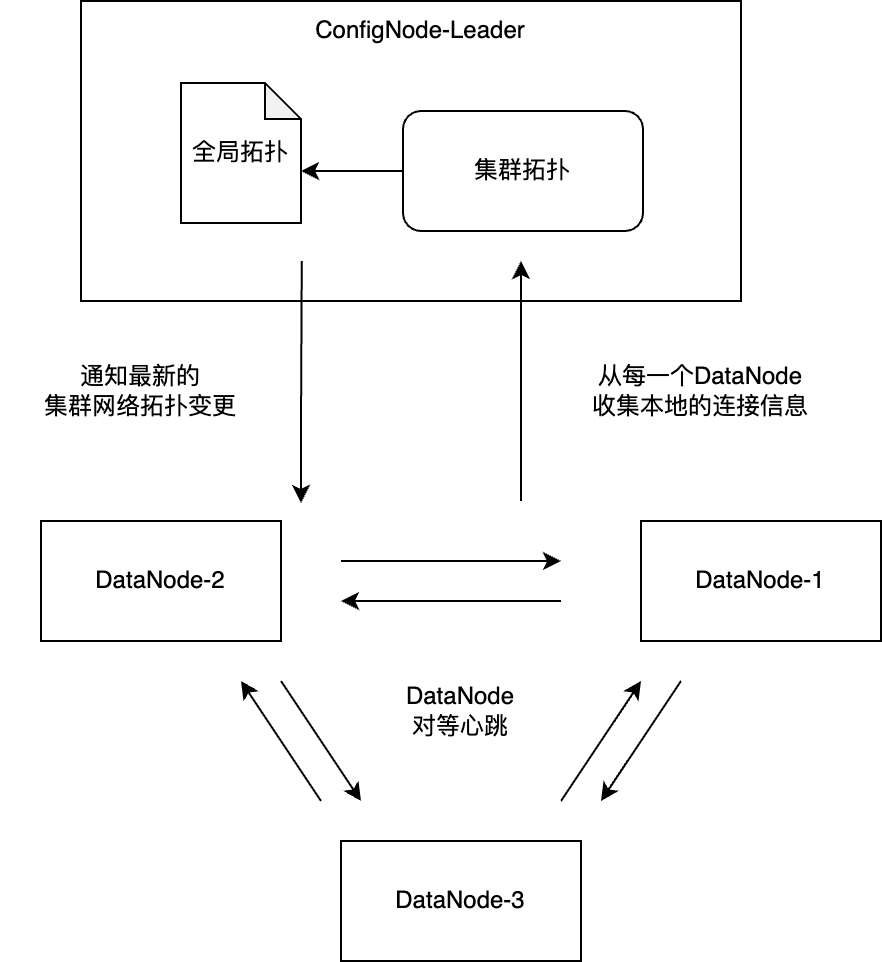
\includegraphics[width=0.8\linewidth]{c03-topology-redraw.png}
  \caption{集群拓扑感知能力}
  \label{fig:c03-topology}
\end{figure}

图\ref{fig:c03-topology}给出了数据节点间的对等心跳机制描述。

管理节点会定期要求集群中的每个数据节点都与其他数据节点进行对等的心跳交换。通过这种全互联的心跳机制,每个数据节点能够更直接地获取自己与其他数据节点性状态,例如是否能够成功发送心跳、是否能够及时收到对方的心跳响应等。

随后,每个数据节点会将自己收集到的与其他数据节点的连通性信息进行汇总和整理,形成一个局部的网络拓扑视图。这个视图包含了该数据节点对集群中其他数据节点可达性的判断。

为了获得全局的视角,每个数据节点会将这个汇总后的连通性报告定期地上报给当前的管理节点领导者。管理节点领导者作为集群的中央协调者,在接收到来自所有数据节点的连通性报告后,便能够汇总所有节点的局部视图,从而构建出一个完整的、全局的集群网络拓扑感知能力。与仅仅依赖管理节点和数据节点之间的单向心跳相比,这种方式能够更全面地了解集群内部节点之间的双向通信状况。

在获取了全局视角的网络拓扑图之后,管理节点会通过RPC的方式将这个全局拓扑下放通知给所有的数据节点,从而赋予每一个数据节点更加完善的集群状态感知能力,允许在后续的写入规划、查询规划等操作更加智能、可靠。

\subsection{客户端节点感知其他节点状态}

客户端会对集群的数据节点状态有所感知,这个感知是两阶段的过程,首先,它依赖于从管理节点获取最新的、潜在可用的数据节点列表及其地址;然后,它通过主动尝试与目标数据节点建立连接来直接验证该数据节点在客户端视角下的实际可达性和存活状态。

客户端并不会预先硬编码所有可能的数据节点地址。相反,客户端在初始化或需要更新集群视图时,会首先与管理节点集群建立连接。管理节点 集群作为整个 IoTDB 分布式系统的元数据管理者,维护着最新的集群拓扑信息,包括当前注册在集群中的所有数据节点的网络地址。

客户端通过后台线程定期(通常是60s)向管理节点拉取当前管理节点认为活跃或已知的数据节点列表及其对应的通信地址。

获取到数据节点列表后,客户端并不会向所有数据节点发送请求。当客户端需要与某个特定的数据节点进行交互时,客户端会尝试与该数据节点的网络地址建立Thrift连接并发送交互请求。如果请求成功,那么客户端会认为该节点存活状态良好。反之,客户端会判断该节点当前不可用。

\section{基于状态感知的故障检测算法}\label{failure_detection}

\subsection{固定心跳超时判断}\label{failure_detection_timeout_fix}

在本文的工作之前,IoTDB内部采用基于心跳固定超时时间的故障检测。该算法可以概括为,如果节点在超过一段时间之后没有收到另外一个节点的心跳,那么就会认为另外的这个节点出现了故障,可能是网络分区或者进程宕机。
更具体地,我们定义超时时间参数$\Delta_{t}$(默认为20s),该参数的含义是:当管理节点领导者在超过$\Delta_{t}$的时间里面没有收到某一个被询问方数据节点的心跳,或者发起方数据节点在超过$\Delta_{t}$的时间里没有收到另外的一个被询问方数据节点的心跳,就会判断被询问方的数据节点不可达,可能是出现了网络分区或者其他问题。

这种基于心跳的固定超时算法的优点在于逻辑简单直接,易于实现和部署,并且在IoTDB已有的实践中能胜任大部分的错误发现。然而这种算法依然存在诸多问题,例如:

1. 固定的算法无法应对复杂和变化的系统环境。节点的网络变化、系统的负载变化、长时间的GC等诸多因素都有可能导致心跳包被延迟传输或拥塞,从而出现超时产生误判,触发不必要的容错操作。

2. 选择一个$\Delta_{t}$ 的最佳参数在实践中非常困难。一方面,参数的选择需要人工介入,需要用户对自身业务集群的特性、IoTDB内核的故障检测机制都有所了解,这对很多用户来说是一个很大的心智负担。
另一方面,参数 $\Delta_{t}$ 本身就是故障检测的检测速度和检测正确度的权衡。选择一个较短的$\Delta_{t}$参数,那么节点故障会被快速发现,但对应的误报率就会很高;如果选择一个较长的$\Delta_{t}$,虽然误报率会对应下降,但是错误的平均发现时间将会变长。

\subsection{Phi Accrual算法判断}

章节\ref{sec:cassandra-failure-detecttion}提到的Phi Accrual能够良好解决上述的两个问题。然而,Phi Accrual算法存在冷启动的问题。在节点启动、重启的阶段,如果错误地将节点判断成不可达,那么可能会导致不必要的\failover 、节点延迟加入集群或提供服务和增加运维复杂性等问题。

为此,本文最后提出的IoTDB故障研判算法是结合心跳固定超时时间的判断和Phi Accrual算法的结果。具体来说,IoTDB的故障检测将会根据节点的生命周期划分为两个阶段:冷启动阶段和正常服务阶段。

冷启动阶段。当节点刚刚启动,或是刚刚从故障恢复,此时我们尚未收集到足够的心跳样本,我们将会使用\ref{failure_detection_timeout_fix}提到的算法来负责初始时期的节点故障检测,并同时在后台继续收集样本。当我们收集了足够的样本数量(默认为60个)的时候,我们切换成基于Phi Accrual的算法来研判节点的存活率。由于节点在刚启动过程中往往不会立马承担较大的流量负载,也不太可能会发生长时间的垃圾回收等异常情况,因此在这个阶段使用固定超时算法将能较为有效地实现故障检测。

节点正常服务阶段。当节点稳定提供服务一段时间之后,我们已经收集到了足够的心跳历史样本,IoTDB集群将会切换为基于Phi Accrual的检测算法进行故障研判。具体的实现如下:

1. 收集心跳历史采样。对于每一个新到达的心跳包,算法会计算出和上一个心跳包之间的间隔,并将这个间隔存入一个固定大小(默认为100)的采样窗口内。当有新的心跳不断到达的时候,最新的一个间隔会被存入采样窗口,窗口最早的第一个间隔则会被剔除,以便更好地反映集群的近况。

2. 根据采样窗口计算到达间隔的分布,计算 $\phi$ 值。在Phi Accrual算法中, $\phi$ 值代表了一个节点出现故障的怀疑概率。
我们假设心跳到达间隔的分布符合正态分布,那么可以通过历史采样窗口来估计分布的均值 $\mu$ 和方差 $\sigma^2$。那么,在上一次心跳到达t时间之后才会有下一次心跳到达的概率可以通过下列公式计算出来:

$$ P_{later}(t) = \frac{1}{\sigma\sqrt{2\pi}} \int_{t}^{\infty} e^{-\frac{(x-u)^2}{2\sigma^2}} dx $$

在实际实现中,我们通过逻辑斯蒂分布对高斯分布进行近似\cite{bronvstejn2013handbook}:

$$ P_{later}(t) = \exp(1.5976 + 0.070566 (\frac{t-u}{\sigma})^2) $$

3. 计算 $\phi$ 并根据设定阈值进行比较。我们使用如下的公式进行定义:

$$ \phi(now) = -log_{10}(P_{later}(t_{now} - t_{last})) $$

用户可以通过设定不同的$\phi$阈值来控制研判的精准度。阈值越高,研判的精准度越高。在章节\ref{sec-experience-phi-accrual}中,我们给出了这个故障检测算法的实验验证和不同阈值参数下算法的表现行为。


\subsection{Thrift连接状态判断}\label{thrift-detection}

在\ref{failure_detection}中提到的故障研判,通过对心跳行为建立概率模型来判断节点是否发生故障。这种故障研判需要一定的观察窗口才能作出可靠的判断,因此发现故障通常需要十秒或者更久。

然而,在进程宕机、被系统强制关闭等特殊场景下,我们可以利用Thrift 长连接的特点,将被动的故障发现转化为主动的故障通知,从而显著加快故障的发现和传播速度。

IoTDB内部采用Thrift\cite{slee2007thrift}框架作为RPC通信的实现。Thrift框架底层使用网络协议层的TCP协议或者UDP协议实现实际的传输。IoTDB 内部采用 ClientManager 接口来统一管理对外的 Thrift 连接。ClientManager 的基本原理类似于带缓存的连接池。当我们首次请求连接到某一个新的 EndPoint(代表一个特定的 IP 地址和端口)时,ClientManager 会建立一个底层的 TCP 连接。与使用完毕后立即断开连接不同,ClientManager 会在结束使用后继续维持这个 TCP 连接一段时间,并将其缓存在本地。这样,在下次我们需要请求相同的 EndPoint 地址时,就不需要重新进行 TCP 三次握手等连接建立的开销,可以直接复用 ClientManager 内部缓存的现有连接。只有当某个 TCP 连接长时间没有被使用时,ClientManager 才会主动销毁该连接并清理相关的系统资源。

由于管理节点和每一个数据节点之间存在持续频繁的内部 RPC 通信,通过上述所言的 ClientManager 的机制,我们可以认为在管理节点和数据节点之间建立了一条长期有效的 TCP 连接信道,并在这个 TCP 信道的基础上建立了一个长期有效的 Thrift 连接。

Thrift框架能够感知其底层的TCP传输层的连接状态。当连接的进程突然出现故障,无论是是由于程序崩溃,还是被操作系统强制终止(例如使用 kill -9 命令),该进程所建立的TCP连接也会中断。
Thrift 能够迅速检测到这个信道的问题,并向上层的IoTDB模块汇报连接中断的事件。
这种主动汇报机制的时间延迟通常在故障发生的毫秒到秒级,非常快速。

管理节点领导者会利用这样的机制,在收到断开汇报的时候将该进程标记为失效,从而实现进程失效的快速检测和优化。

\section{本章小结}

本章详细阐述了 Apache IoTDB 分布式集群高可用与容错框架的集群故障检测和判断机制部分。及时、准确地感知故障是系统能够实施有效恢复和转移策略的前提。

章节首先描述了不同角色节点间的状态感知方式。


管理节点 作为集群的“大脑”,通过与管理节点之间基于 Raft 协议的心跳以及与数据节点之间定期的 RPC 心跳,周期性地收集集群各成员的基本存活状态、资源负载等信息。同时,数据节点之间也通过对等心跳进行连通性探测,并将结果上报给管理节点,增强了集群对内部网络状况的感知能力。客户端客户端则通过尝试建立和维持与数据节点的连接来判断其可达性。

在此状态感知的基础上,本章着重探讨了用于研判节点故障的算法。章节回顾了传统固定心跳超时算法的优缺点,指出其在复杂多变网络环境下易产生误判且参数难以调优的问题。进而引入并详细阐述了更具适应性的 Phi Accrual 算法,该算法通过分析心跳历史,以概率形式(Φ 值)判断节点的怀疑度,能够更精确地反映节点存活状态。考虑到 Phi Accrual 算法在冷启动阶段的不足,本章提出了一种结合策略:在节点冷启动阶段采用固定超时判断快速发现早期问题,在进入正常服务阶段后切换至基于 Phi Accuarl 算法进行更鲁棒的故障研判。
% !TeX root = ../thuthesis-example.tex

\chapter{集群故障容错和恢复}

\section{基于拓扑感知的查询和写入规划}
上文提到了集群的拓扑感知,总结来说,ConfigNode Leader不但可以探知每一个节点的存活情况,还能够探测DataNode之间的每一个连接。当发现出现网络分区和节点宕机等情况的时候,本文提出的高可用解决办法可以通过对查询和写入规划的改写和三级重试来做到最大限度的错误避免和自动容错,从而保证用户的请求依然能够完成。本节主要介绍基于拓扑感知的查询流程。

\subsection{写入和查询流程概述}

\begin{figure}
  \centering
  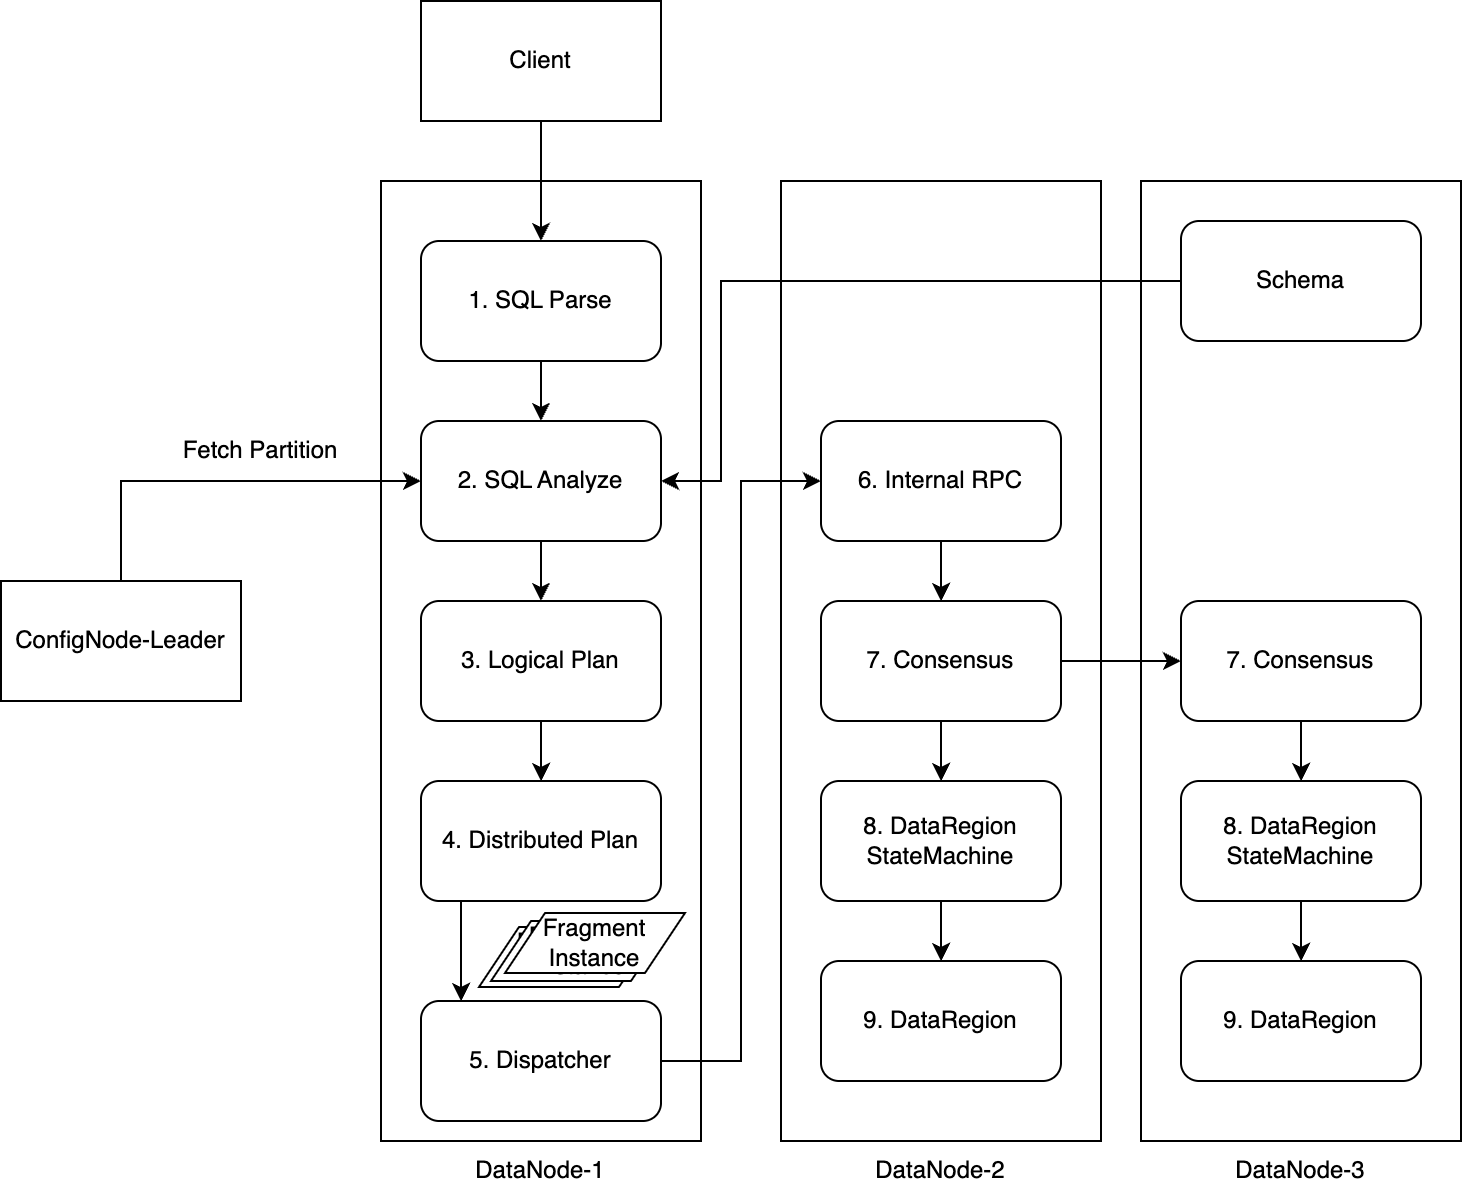
\includegraphics[width=0.99\linewidth]{c04-write-process.png}
  \caption{IoTDB写入全流程}
  \label{fig:c04-write-process}
\end{figure}

图\ref{fig:c04-write-process}展示了IoTDB现有的写入和查询流程。

首先,客户通过SQL等方式请求IoTDB的DataNode,从而发起写入或查询流程。目前,IoTDB集群中的所有DataNode都能对外提供同质化的写入和查询服务,客户端可以选择连接在任意一个DataNode上发出写入的请求。

当客户端的SQL请求到达IoTDB的DataNode之后,第一步会首先对客户端发送的SQL进行解析(SQL Parse)。这一步主要会对SQL进行语法和格式的校验等。

接下来第二步会进入分析阶段(Analyze),本阶段主要准备本次写入或查询执行所需要的数据,主要包含两部分:元数据和集群Region的分区数据。DataNode可能会从ConfigNode这里请求所需要的最新的分区情况,并从其他的DataNode上拉取所需要的元信息。在此步骤上还会校验相关的数据。

在所有的信息都准备到位之后,第三步会进行逻辑计划的生成(Logical Planning)。逻辑计划描述了查询的逻辑操作,但不涉及具体的物理执行细节。逻辑计划通常以树形结构表示,称为逻辑查询树,树的每个节点代表一个逻辑操作符,例如选择、投影、连接、聚合等,树的边表示数据的流动。

有了逻辑计划之后,第四步会进行分布式执行计划的生成(Distributed Planning)。分布式计划是在逻辑计划的基础上,考虑集群数据分布和并行执行的计划方案,它描述了如何在分布式环境中执行查询,包括数据如何在节点上传输、没有依赖的操作可以在哪些节点上并行执行等。
分布式计划的基本组成单元是碎片实例(FragmentInstance)。它代表了分布式执行计划中针对某一个分区Region的操作。每一个FragmentInstance能够保证在一个分区执行内完成,不涉及跨分区的数据搬运。

产生了分布式执行计划之后,第五步就是由调度器去实际调度和执行分布式计划的每一个碎片实例。根据写入或者查询规划的不同,调度器可能将碎片实例调度到本地直接执行,也可能将实例调度到远端执行。如果调度失败,调度器还可能会重试调度。

在理想情况下,每一个实例最终会被交付给共识层进行执行。共识层会进行相关的读写操作的执行,并且提供数据复制和一致性的保证。以Raft共识协议为例,交给共识层的写入操作会保证被复制给大多数节点执行完成之后才会返回成功写入,交给共识层的读取操作能够保证读到线性一致性的结果。

真正执行操作的是IoTDB的单机存储引擎,采用LSM架构\cite{o1996lsmtree},使用MemTable作为内存结构,使用TsFile\cite{zhao2024apachetsfile}作为持久性外部存储。

\subsection{基于拓扑感知的写入流程优化}

在2.0.2.1版本之前,对于需要调度器在远端调度的写入碎片实例,如果写入失败,调度器会进行多次重试,直到达到客户端配置的请求超时时间之后才会返回客户端失败。在网络分区的情况下,客户端的请求可能需要在很长时间的重试之后依然失败。如果在客户端侧没有配置重试的策略,那么这就将会导致这种情况下的客户端数据丢失,RPO不为0的情况。

在拓扑感知的情况下,我们采用了立马失败的策略。当我们检测到网络分区判断出本次执行必将失败的时候,我们会直接在调度之前就失败。

\begin{figure}
  \centering
  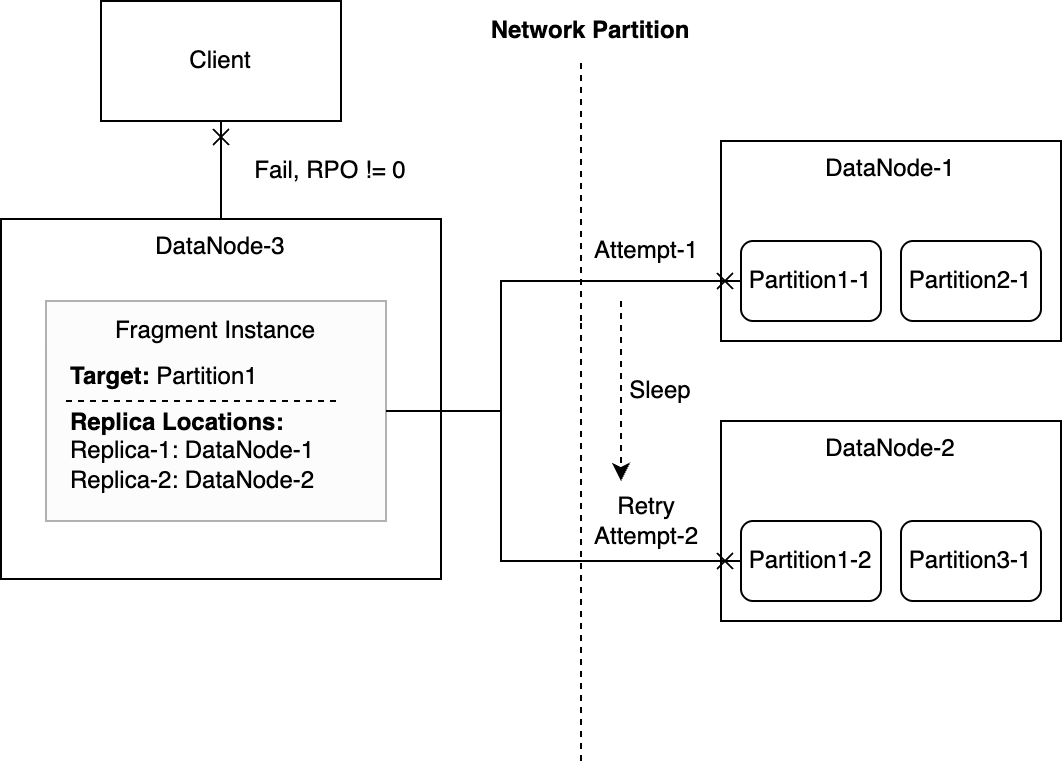
\includegraphics[width=0.9\linewidth]{c04-write-with-topology.png}
  \caption{网络分区下的写入失败情况}
  \label{fig:c04-write-with-topology}
\end{figure}

在\ref{fig:c04-write-with-topology}图中我们可以看到分区的问题。
在IoTDB的集群中,DataNode3和其他两个节点产生了对称分区问题。此时,如果Client连接上了DataNode3执行写入计划,写入计划最终会被解析为FragmentInstance,对象是Partition1。但是不巧的是,Partition1的两个副本分别在DataNode1和DataNode2上,这导致了这个FragmentInstance需要被调度到这两个节点上执行。
在2.0.2.1方案之前,调度器会先尝试调度到DataNode1上,但是由于网络分区的问题,本次请求最终会以超时失败。接着,调度器会尝试选择第二个副本执行,再次尝试调度,但本次请求最终依然会因为分区而失败告终。调度器会反复重复上述的重试策略,直到本次的执行超过客户端指定的超时时间,最终返回客户端失败。

这种写入计划和执行存在两个问题。首先,对于客户端来说,网络分区的错误需要经历一个完整的超时周期(默认配置是1分钟)才会返回,这会严重影响客户端的吞吐。其次,如果客户端不尝试连接其他的DataNode进行重试,那么本次写入失败最终会导致这部分的数据未能被持久化。


在具备拓扑感知功能后,我们可以在规划阶段就解决这个问题。

详细来说,在生成FragmentInstance之后,我们可以提前根据从ConfigNode Leader下发的集群最新拓扑结构对这个FragemntInstance涉及的Partition的所有地点进行可达性计算。如果有些副本所在的节点因为分区等原因不可达,那么就会标记这些副本,在调度的时候避开这些位置。
如果一个FragmentInstance的所有副本位置都不可达,那么调度器就不会调度,而是直接返回客户端这个FragmentInstance写入失败。客户端此时可以配置重试策略,将本次写入请求连接到DataNode-1或者DataNode-2上进行执行,最终实现写入。
总结来说,在具备拓扑感知能力之后,写入请求不会进行长时间的重试,能够立马发回客户端重试。同时,返回时会带上建议的重试节点,帮助客户端完成最后的写入。

\subsection{基于拓扑感知的查询流程优化}

\begin{figure}
  \centering
  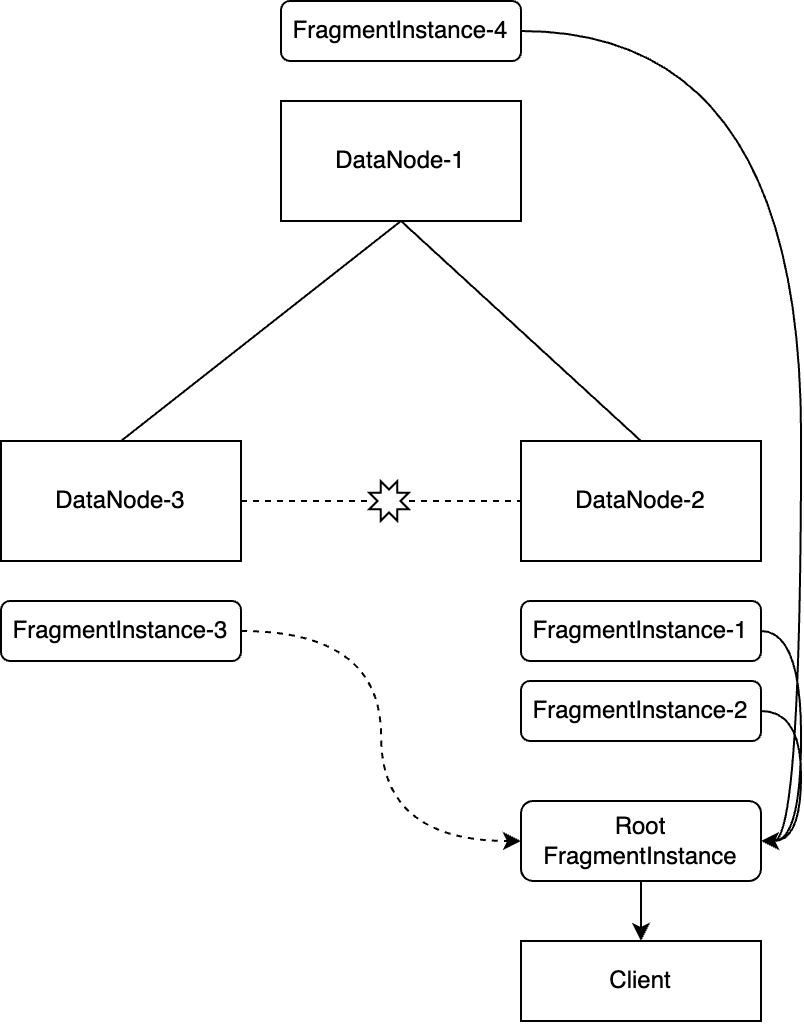
\includegraphics[width=0.7\linewidth]{c04-fi-topology-partition.png}
  \caption{网络分区下的查询失败情况}
  \label{fig:fi-topology-partition}
\end{figure}

在非对称网络分区的情况下,例如图\ref{fig:fi-topology-partition}所示,没有拓扑感知的查询规划可能会导致在资源允许的条件下依然查询失败的错误。在分布式查询计划中,root fragment instance是位于查询计划的顶端的节点,负责最终结果的聚合,需要收集其他碎片实例的结果,也是最终返回结果的那个计算节点。

例如图中所示,本次查询计划涉及4个FragmentInstance,分别会被调度到DataNode的1,2,3节点上实现。本次查询的root instance 被调度到了DataNode2上,出于最小化数据在节点之间传输的考虑。在DataNode2和DataNode3之间发生非对称网络分区的时候,DataNode-2上的root Fragemtn Instance并不能成功连接DataNode3并且拉取对应的数据,这导致了本次查询的失败。

在有了拓扑感知算法之后,本次查询规划的时候可以把root FragmentInstance调度到DataNode1节点上,这样即使在出现了非对称网络分区的情况下,DataNode1依然可以连接到剩下的两个节点,位于DataNode1上的root FragmentInstance可以成功拉取本次查询规划的所有的instance的数据。

再次我们给出基于网络拓扑分区的root fragment instance的算法描述。
\begin{algorithm}
  \caption{查找DataNode和FragmentInstance候选}
  \label{alg:find_candidates}
  \begin{algorithmic}
  \REQUIRE 集群拓扑结构 (连通图), FragmentInstance列表
  \ENSURE DataNode候选列表, FragmentInstance候选列表
  
  \STATE $DataNodeCandidates \leftarrow \emptyset$
  \STATE $FragmentInstanceCandidates \leftarrow \emptyset$
  
  \FOR{每个 DataNode $node$ 在 集群拓扑结构 中}
      \STATE $isCandidate \leftarrow true$
      \FOR{每个 FragmentInstance $instance$ 在 FragmentInstance列表 中}
          \STATE $foundConnection \leftarrow false$
          \FOR{每个 Replica $replica$ 在 $instance.ReplicaSet$ 中}
              \IF{$node$ 和 $replica$ 在 连通图 中连通}
                  \STATE $foundConnection \leftarrow true$
                  \STATE \textbf{break} \COMMENT{找到一个连接即可}
              \ENDIF
          \ENDFOR
          \IF{$foundConnection = false$}
              \STATE $isCandidate \leftarrow false$
              \STATE \textbf{break} \COMMENT{如果和任何ReplicaSet都无法连通,则不是候选}
          \ENDIF
      \ENDFOR
      \IF{$isCandidate = true$}
          \STATE $DataNodeCandidates \leftarrow DataNodeCandidates \cup \{node\}$
      \ENDIF
  \ENDFOR
  
  \FOR{每个 FragmentInstance $instance$ 在 FragmentInstance列表 中}
      \STATE $isCandidate \leftarrow false$
      \FOR{每个 DataNode $candidate$ 在 $DataNodeCandidates$ 中}
          \FOR{每个 Replica $replica$ 在 $instance.ReplicaSet$ 中}
              \IF{$candidate = replica$}
                  \STATE $isCandidate \leftarrow true$
                  \STATE \textbf{break} \COMMENT{找到一个候选DataNode即可}
              \ENDIF
          \ENDFOR
          \IF{$isCandidate = true$}
              \STATE \textbf{break} \COMMENT{找到一个候选DataNode即可}
          \ENDIF
      \ENDFOR
      \IF{$isCandidate = true$}
          \STATE $FragmentInstanceCandidates \leftarrow FragmentInstanceCandidates \cup \{instance\}$
      \ENDIF
  \ENDFOR
  
  \RETURN $DataNodeCandidates$, $FragmentInstanceCandidates$
  \end{algorithmic}
  \end{algorithm}

\section{错误时期的三级重试和Failover}

为了确保系统在面临各种故障时仍能保持高可用性和数据一致性,我们采用了一种基于重试的故障转移策略。具体而言,我们设计了一种三级重试机制,该机制涵盖了客户端、协调者以及共识层。通过在这些关键层面上实施重试,我们旨在最大程度地提高错误恢复的成功率,确保即使在不利条件下,系统也能正确处理并解决问题。这种多层次的重试策略不仅增强了系统的鲁棒性,还显著提升了其在复杂分布式环境中的可靠性。

整个三级重试的的实现方案。

\subsection{Session的重定向重试}

在Apache IoTDB中,Session扮演着至关重要的角色,它不仅是客户端应用程序与IoTDB DataNode集群之间进行通信的桥梁,更是实现服务自动发现的关键组件。具体来说,Session封装了与IoTDB服务器建立连接、发送请求、接收响应等一系列底层操作,为应用程序提供了简洁高效的API接口。通过Session,客户端能够轻松地执行数据写入、查询、元数据操作等任务,而无需关心复杂的网络通信细节。此外,Session还具备自动发现DataNode集群服务的能力,这意味着即使集群拓扑结构发生变化,客户端也能自动适应并保持与可用节点的连接,从而确保了系统的高可用性和稳定性。值得注意的是,Session的设计充分考虑了性能和安全性,它通过连接池等机制来减少连接建立的开销,并通过身份验证和权限控制等手段来保障数据的安全性。因此,Session是IoTDB客户端应用程序开发中不可或缺的核心组件。

Session侧的重试是高可用的重要组成部分,是DataNode服务发现和负载均衡的基础。通常来讲,客户端依赖Session连接到集群中的某一个特定DataNode上执行相关的操作请求。然而,如果该DataNode节点突发故障,例如进程宕机、因网络分区而导致连接中断、高负载状态下导致资源耗尽而不能很好地提供服务,此时Session就能通过执行超时和连接通道来检测出异常的发生,并启动故障转移的流程,将请求自动连接到其他的节点中完成。
通过这种无缝切换,Session不但保证了客户端的请求能够被路由到健康的节点上执行,从而保证了数据写入操作的正确性和可靠性,也同样实现了负载均衡的能力。

每一个Session启动的时候,都会配置至少一个DataNode节点和ConfigNode的节点。在Session创建之后,会启动一个后台的进程,这个进程会从集群的大脑ConfigNode中定期拉取所有DataNode的列表和其对应的状态。当当前的DataNode出现问题的时候,Session就会根据列表的顺序不断尝试下一个可用的DataNode。这种实现方式还有一个额外的好处。当集群增加一个新的DataNode的时候,不需要对现在存活的Session进行修改配置并且启动,这个机制能够自动让现有的Session发现这些新增的DataNode,并将数据引导到新的DataNode上。

DataNode在写入的时候,还会进行Redirect的提示,这个行为是集群自动负载均衡的重要能力之一。Session在初始创建的时候,可以默认连接到任何一个DataNode上。当DataNode处理完了这个连接的请求的时候,会根据集群的综合情况考虑,在返回结果的地方增加一个建议重定向的字段,该字段的用意是希望Session后续的连接能够重定向到其他节点上来执行。在处理带有重定向标志的Session的时候,Session会将底层的连接信道重新导引到那个新的DataNode之上,通常,当需要读写的副本的leader节点所在DataNode的时候,才会发生这样的重定向导引活动。

此外,在出现了上述提到的非对称网络分区的时候,查询规划和计划也会建议重定向。如上述所言,如果在非对称分区的时候rootInstance没有地方摆放,那么返回给Session的报错信息就会加上重定向的DataNode,这个DataNode往往能够放置这个root instance。


总结来说,Session侧的重试实现了服务发现、自动转移、负载均衡和容错的能力。



\subsection{协调者}

协调者(Coordinator)是IoTDB的重要组成部分,他负责接受客户端的SQL请求,负责SQL解析、物理计划和分布式执行计划的生成,对每一个FragmentInstance进行调度和执行,以及最终结果的的收集和返回。

协调者侧重试的目的是避免因为单副本、单节点的失效而影响查询和写入的能力。通过充分利用底下共识模块提供的多副本的能力,协调者能够在某个副本写入失败的时候自动转移到另外一个副本上,从而规避系统的暂时性错误。






\subsection{Client的重试策略}




\section{共识模块}


在Apache IoTDB中,共识模块是构建高可用能力和故障容错能力的基石。数据管理、元数据管理、ConfigNode的服务都依赖共识模块。

共识层的核心目标在于为同一份数据维护多个满足一致性要求的数据副本,这种多副本的能力不但是抵御故障、实现系统自动容错能力的基础,更是构建负载均衡、节点迁移和扩缩容等高级功能的前提。

对内,共识层隐藏了数据副本同步和一致性维护的诸多挑战,包括数据的异步复制、周期性的数据检查与校验、网络波动下的断点续传、以及可能出现的数据冲突和解决策略,通过一致性算法确保即使在网络分区、节点故障等异常情况下,所有数据副本都能在最终保持高度一致。

对外,共识层的多副本抽象简化了上层依赖模块的开发工作。对于写入模块而言,它无需关注底层数据同步的细节,只需要写入一个副本即可。对于查询引擎而言,它可以放心地从任意一个副本读取数据,并确保读取到的数据满足系统定义的一致性条件。


\subsection{统一框架下的不同协议}

共识模块定义了一系列标准化的接口,包括创建和销毁数据副本、执行读写操作、以及进行成员变更等,从而实现了共识模块的插拔能力,允许使用者通过配置的方式灵活选择不同的共识协议实现。
共识模块依赖复制状态机\cite{lamport1978statemachine}(replicated state machine)的规范实现标准化。实现了复制状态机接口的包括存储引擎DataRegionStateMachie,元数据存储引擎SchemaRegionStateMachine和集群中心服务ConfigRegionStateMachine。

目前IoTDB提供了三种不同的共识协议的实现,分别是基于Raft算法的强一致性共识协议RatisConsensus,基于多主复制的会话一致性共识协议IoTConsensus和基于主从快照同步的最终一致性共识协议IoTConsensusV2。

图\ref{fig:c04-consensus-arch} 给出了共识层统一框架的示意图。本节接下去的内容将会简要介绍每一个共识协议的实现和提供的高可用保障级别。

\begin{figure}
  \centering
  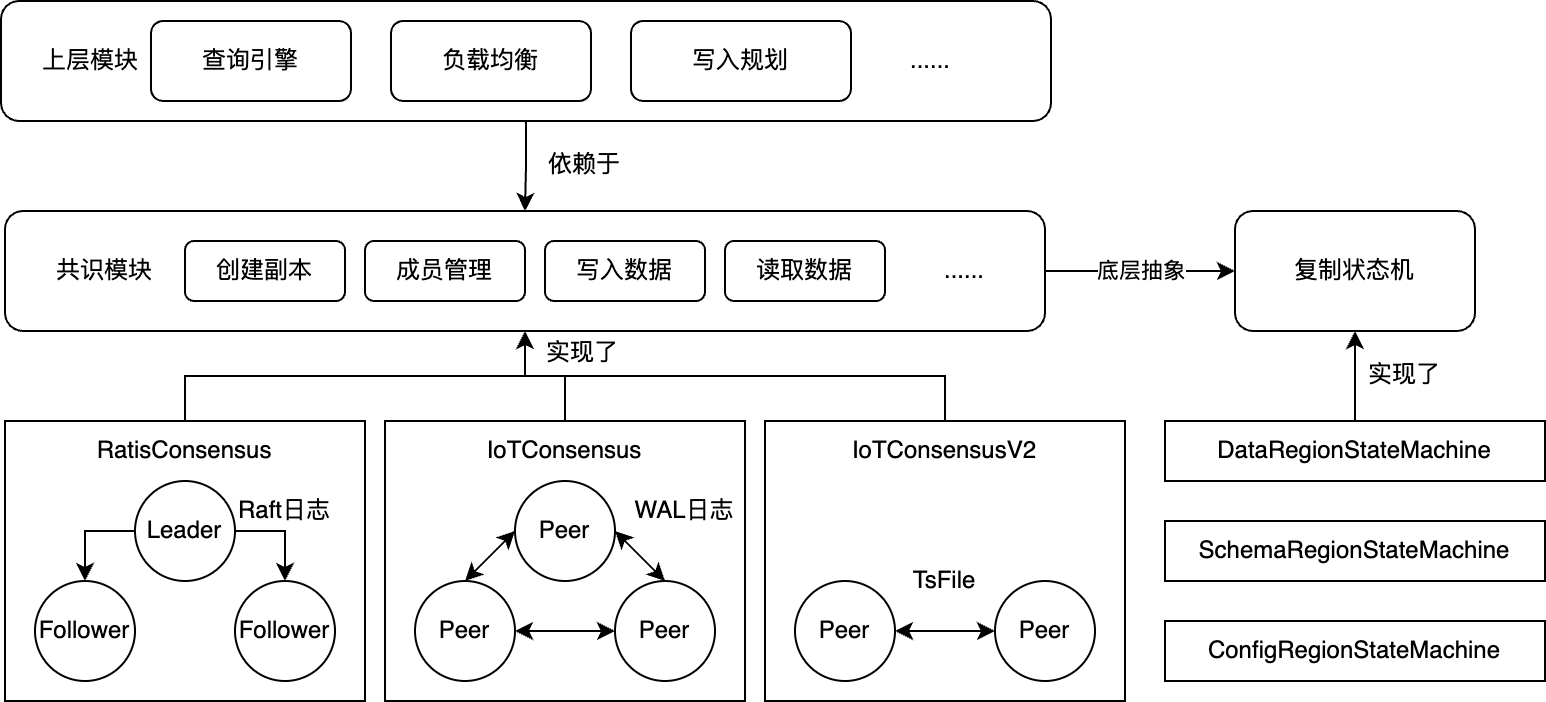
\includegraphics[width=0.99\linewidth]{c04-consensus-arch.png}
  \caption{共识层统一框架架构图}
  \label{fig:c04-consensus-arch}
\end{figure}


\subsection{RatisConsensus}

RatisConsensus是IoTDB提供的强一致性共识协议实现,基于Raft共识算法和Apache Ratis\cite{ratis}开源项目实现。目前,RatisConsensus是集群元数据管理和ConfigNode服务默认的共识协议。

RatisConsenus内部会维护奇数(2N+1,默认为3)个副本,并为每一个副本提供线性一致性的语义保障。由于底层依赖的Raft算法是基于单主复制结构的共识协议,因此在任何时刻,这些副本只有一个可以接受上层的写入请求,被称为Leader副本,剩下节点从Leader副本同步数据,可以接受只读请求。
RatisConsensus能够自动容忍少数副本的失效依然保持数据和服务的可用性。具体来说,对于一个2n+1副本的RatisConsensus服务,最多能够容忍n个副本的失效。同时,RatisConsensus能够保证在网络分区情况下的数据一致性,同一时刻能保证最多只有一个副本成为Leader 副本。

RatisConsensus底层的一致性协议是Raft算法,包含Leader选举、日志复制和安全性保障等核心要素。Raft通过随机超时来实现Leader选举,通过任期(Term)来保证每次选举的唯一性和权威性。Leader接受写入数据,并将自身日志强制复制给所有Follower,最终所有的日志可以被排列出一个副本之间达成共识的全序序列,不同的副本均按照这个全序序列应用日志,从而实现副本数据之间的一致性。为了确保安全性,Raft 引入了 Commit 机制,即只有在大多数副本上保存了对应日志条目后,该日志才能被 Commit,上层才能收到共识层写入成功的回应。

\begin{figure}
  \centering
  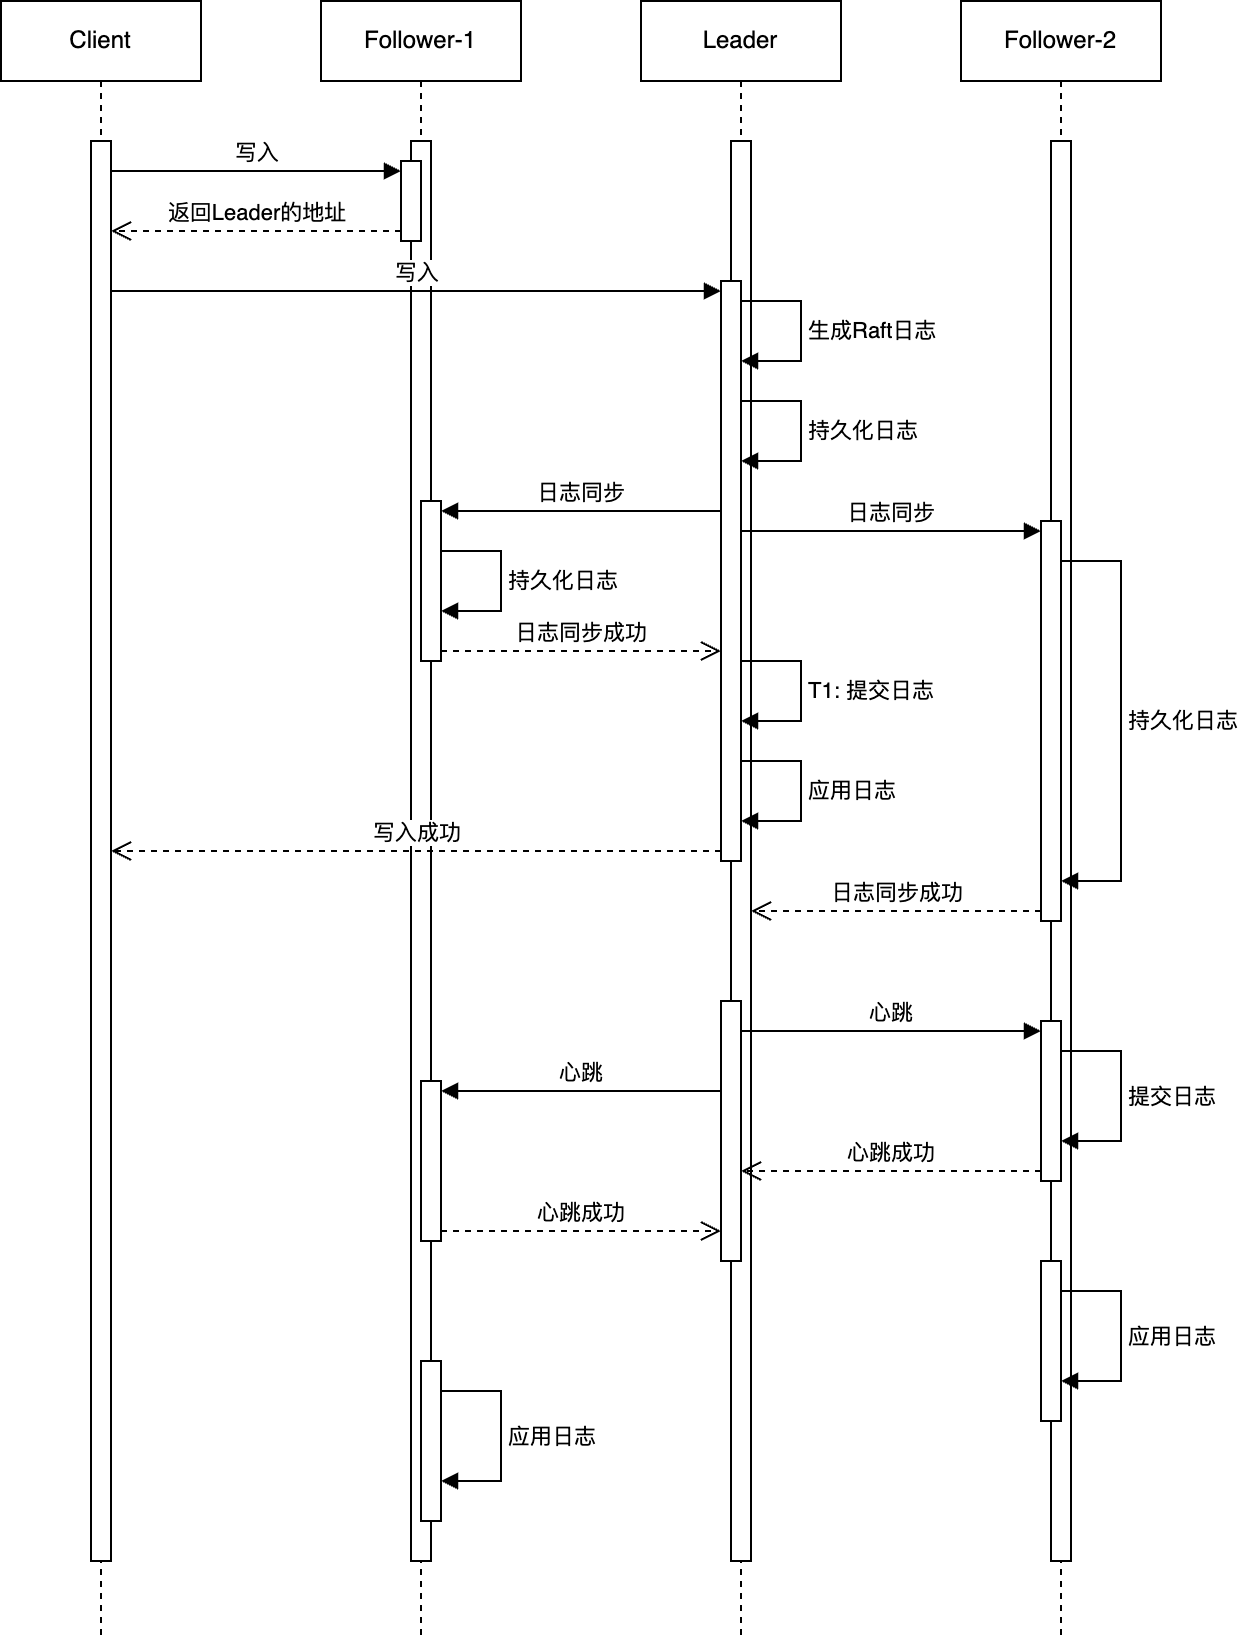
\includegraphics[width=0.6\linewidth]{c04-ratis-write.drawio.png}
  \caption{RatisConsensus数据写入和副本复制流程}
  \label{fig:c04-ratis-write}
\end{figure}

图\ref{fig:c04-ratis-write}给出了一条数据提交给RatisConsensus之后背后的数据复制流程。用户写入数据之后,会由Leader这边负责生成持久化日志并同步到所有节点上,在T1时刻,有超过半数的节点完成持久化同步之后,该操作的状态将会改变成Commit,Leader会应用这个日志并返回对应的结果。Raft算法会在后台保证所有节点能够最终都Commit并应用这个日志。



\subsection{IoTConsensus}

IoTConsensus是IoTDB提供的会话一致性共识协议实现,基于多主异步复制的自研实现。目前,IoTConsensus是集群数据管理的可选共识协议之一。

IoTConsensus的设计初衷是为牺牲一定的可用性换取极致的可用性和更高的性能。
用于在工业物联网场景中,设备不断的时序数据,每台设备的写入请求往
往是串行无重复的,因而并发的写入请求之间通常不存在冲突。因此,IoTConsensus放宽了串形化的一致性约束,允许任何一个副本都能接受读写请求,并且请求在一个副本上执行成功即可返回客户端操作成功。


\begin{figure}
  \centering
  \subcaptionbox{IoTConsensu整体结构\label{fig:c04-iot-arch}}
    {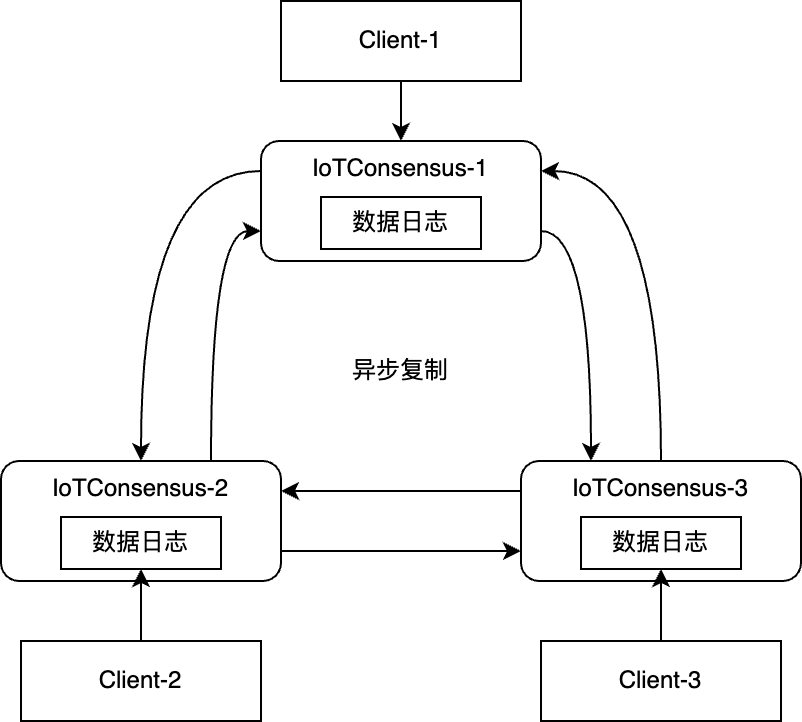
\includegraphics[width=0.4\linewidth]{c04-iot-arch.png}}
  \subcaptionbox{IoTConsensus写入流程\label{fig:c04-iot-write}}
    {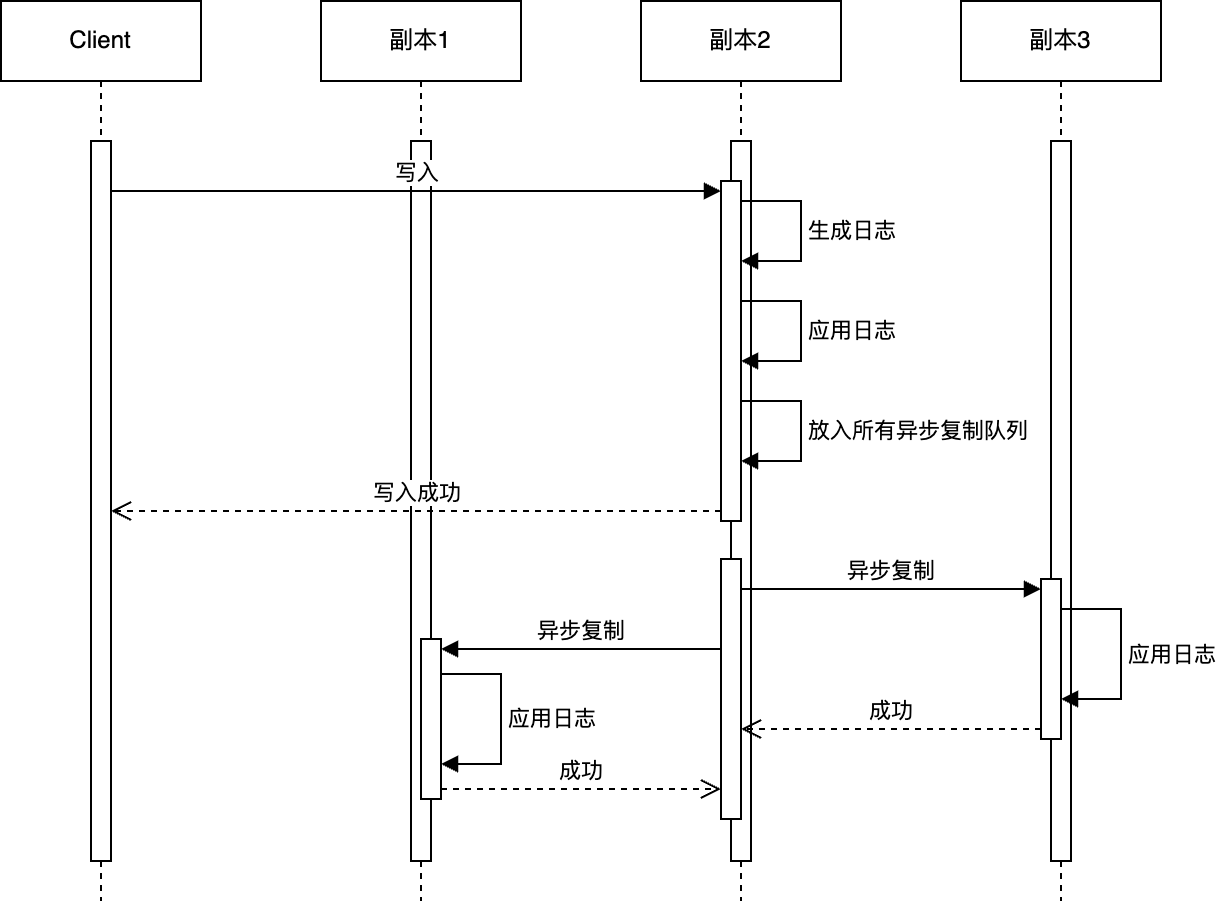
\includegraphics[width=0.58\linewidth]{c04-iot-write.png}}
  \caption{IoTConsensus示意图}
  \label{fig:c04-iot-consensus}
\end{figure}

图\ref{fig:c04-iot-arch}展示了IoTConsensus的结构,允许任何一个副本接受客户端的写入请求,并通过每个节点的后台异步复制线程将写入请求同步给其他的副本。


值得注意的是,当不同副本的数据产生冲突是,可能会导致副本之间数据无法达到最终一致,该问题的解决需要应用层的介入。例如在 Apache IoTDB 中,如果观察到某个序列的数据在不同副本上不一致,则可以使用 Select Into 子句拉取该序列在当前 Leader 副本上的数据并
重新向该共识组流式写入。但在绝大部分的正常应用场景,这种不一致不会发生。


\subsection{IoTCConsensusV2}

IoTConsensusV2是IoTDB提供的最终一致性共识协议实现,基于主从异步复制的自研实现。目前,IoTConsensusV2是集群数据管理的可选共识协议之一。

IoTConsensusV2相较于IoTConsensus相比,进一步牺牲了副本之间的同步时延、一致性级别,换取了极高的写入吞吐。

IoTConsensusV2的总体思路是使用TsFile实现副本之间的数据同步。一般来说,IoTConsensus会设置主从两个副本,并在两个副本之间架设Pipe的通信管道。当主副本的存储引擎每次生成一个TsFile之后,会通过Pipe向从副本同步这个TsFile。整个数据的同步过程仅涉及到常数级别的复杂度操作,同时不用经过 Wal 的磁盘持久化和 Memtable 的内存维护,因此写入吞吐非常高,并且能够解决IoTConsensus存在的由于Follower宕机或Leader节点写入速率大于同步速率导致的WAL文件堆积和写入阻塞的问题。


然而,TsFile的生成相比每一条写入日志需要较长的时间,副本间数据同步延迟可达到几十分钟甚至是几个小时的数据。在两副本的情况下,如果主副本宕机,可能出现由于部分数据还未同步导致的数据暂时丢失的情况。如果宕机节点后续永久没有加入集群,那么这部分数据就会永久丢失。


\begin{figure}
  \centering
  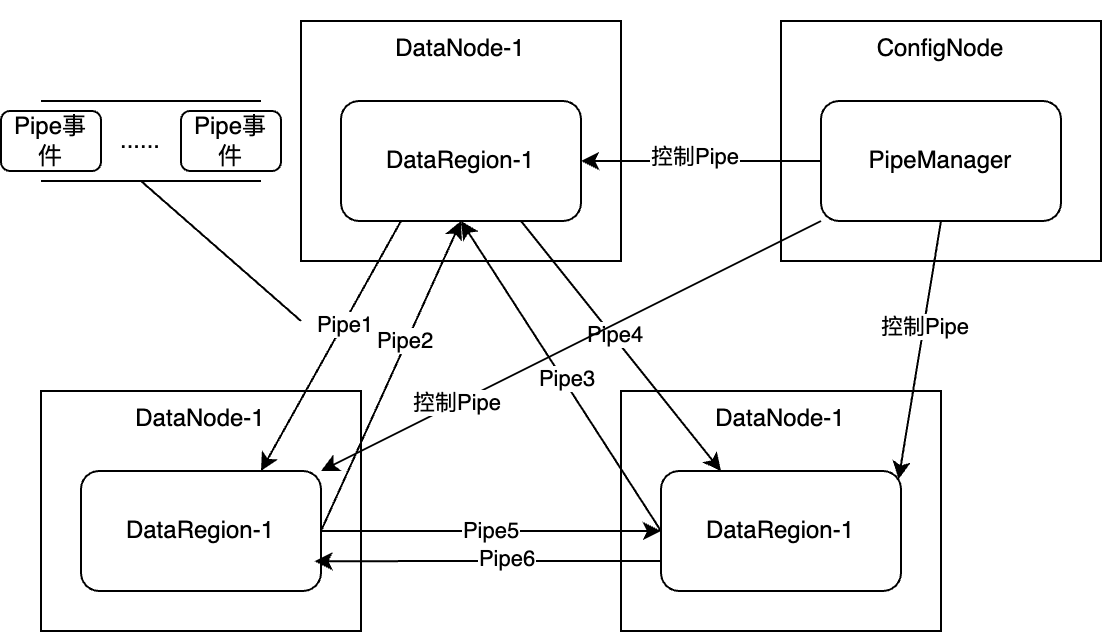
\includegraphics[width=0.8\linewidth]{c04-pipe-consensus.png}
  \caption{R}
  \label{fig:c04-pipe-consensus}
\end{figure}

图\ref{fig:c04-pipe-consensus}给出了PipeConsensus的整体架构。


\subsection{熔断和降级措施}




% !TeX root = ../thuthesis-example.tex

\chapter{经典故障场景分析}

\section{单节点磁盘写满}

\subsection{故障检测方法}

目前IoTDB集群中有两种单节点磁盘写满的故障检测方式。

第一种是定期预防式的诊断,通过ConfigNode和DataNode的心跳完成。ConfigNode和DataNode交换的心跳包中会带有该DataNode节点的磁盘最大容量和目前的使用情况。如果目前的使用率已经超过了预先设置的阈值,那么ConfigNode就会将该节点标志为只读的状态。

第二种是发生时的临诊,通过DataNode在写入过程中的自检来完成。在DataNode服务某一个写入请求在文件系统上真正写入数据之前,会进行可写入性的检查,如果发现此时磁盘空间不足,那么本次写入请求就不会执行,并且返回给Session本次节点只读的状态。

\subsection{高可用容错方案}

\begin{figure}
    \centering
    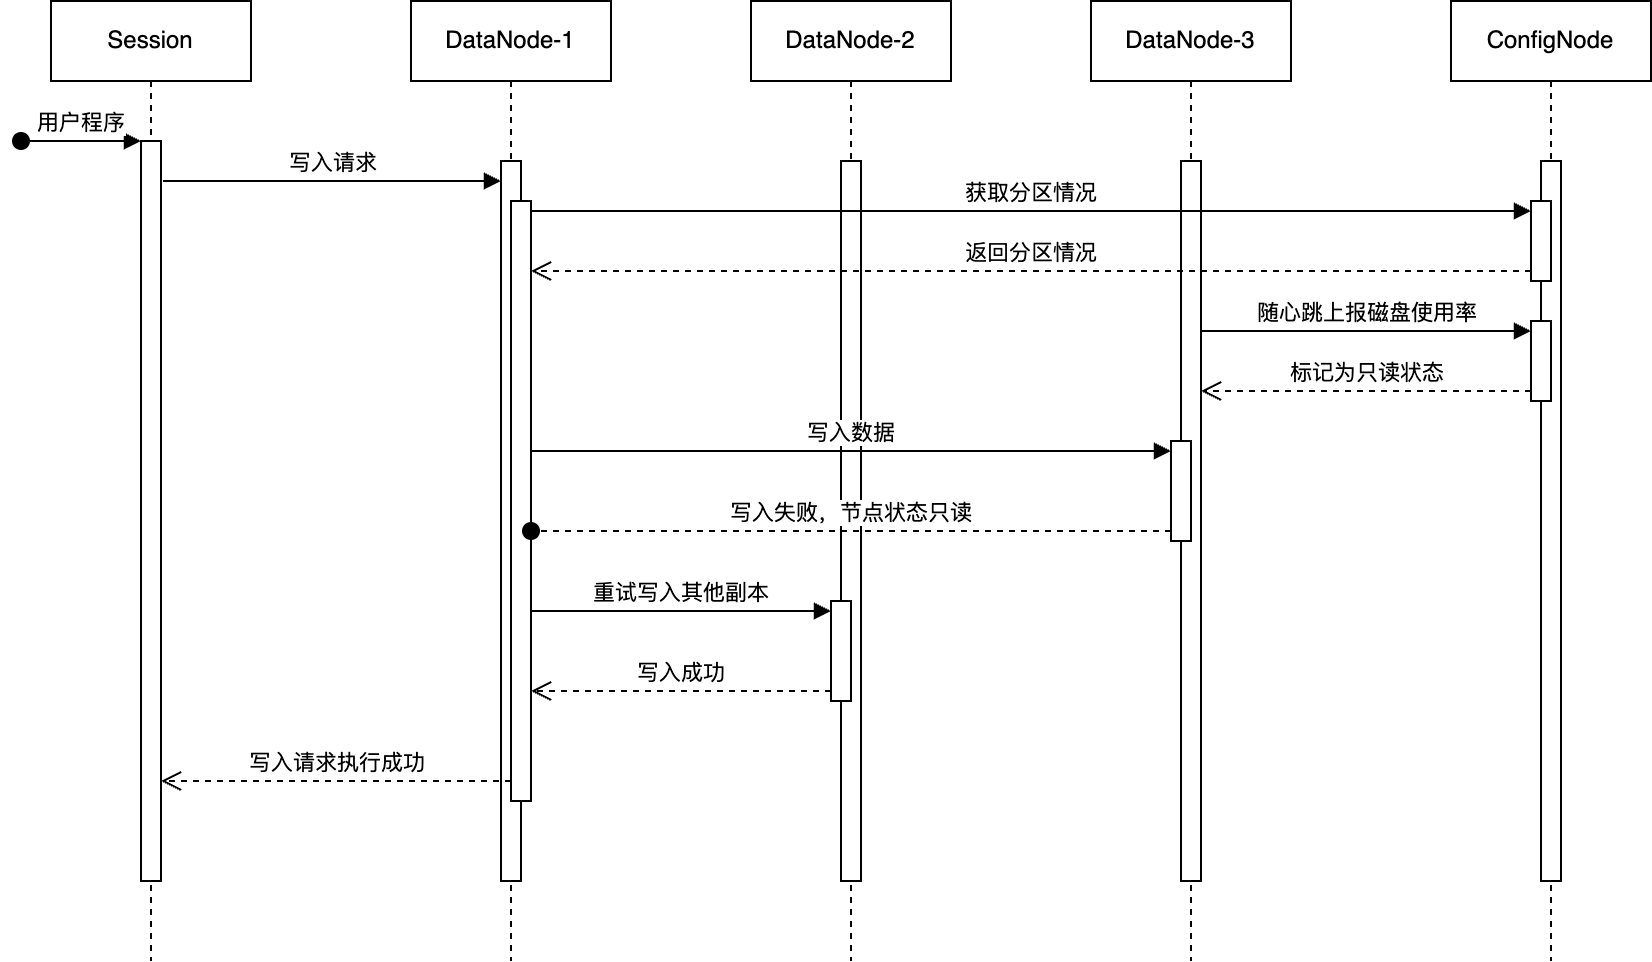
\includegraphics[width=0.99\linewidth]{c05-diskfull.png}
    \caption{单节点磁盘写满的高可用容错时序图}
    \label{fig:c05-diskfull}
  \end{figure}

图\ref{fig:c05-diskfull}给出了单节点磁盘写满的完整容错时序图。

可以看到,再某一个时刻,DataNode3的磁盘使用情况超过了阈值,并且在下一次和ConfigNode上报心跳的时候将这一情况上报给了ConfigNode。ConfigNode会将该节点标记为ReadOnly,并且在后台尝试将该节点上的所有Region的Leader转移给其他的副本,并且标记这些副本的状态为只读。

对于读请求来说,无论是故障发生时的在途请求,还是故障发生之后的新请求,都能够正常执行,不受任何影响。

对于写请求来说,则通过前一章节描述的故障错误转移的方式来实现容错。
对于故障发生之后的写入请求来说,在写入的规划阶段,规划器能够从ConfigNode这边拿到最新的分区情况,此时规划器会将本次的请求给路由到其他可以写入的副本上,从而避免错误的发生。
对于故障发生时就在执行的在途请求,则是通过Session和Coordinator侧的重试来保证数据的正确写入。以图中的写入请求为例,该请求在规划时DataNode3并没有标记为只读状态,因此规划的结果是将数据写入到DataNode3中。然而,在数据写入之前,DataNode3的状态变更为只读,无法再服务外部的写入请求。此时,写入到该节点的操作会返回只读的异常状态,DataNode1会在Coordinator侧捕捉这个错误异常,并且重试。重试时,Coordinator会选择其他的可用副本(在本示意图中为DataNode2),Coordinator会尝试将数据写入正常运行的DataNode2中,最终实现数据的成功写入。


\section{进程宕机}

\subsection{检测方法}
ConfigNode进程宕机和DataNode的进程宕机(kill -9, OOM)等场景下,可以通过ConfigNode Leader建立的心跳通道断开被直接发现。
具体来说,ConfigNode Leader和DataNode之间的心跳通道是基于Thrift构建的,底下的传输方式为Thrift的TSocket,在具体实现中,TSocket是基于TCP实现的。当一个进程突然崩溃或被强制终止时,操作系统会立即关闭该进程打开的所有TCP连接,因此ConfigNode Leader的Thrift连接能够捕获这些TCP层面的信号,立即得知连接已断开,并向应用程序报告。即使TCP连接没有立即断开,如果对端进程已经停止响应,任何尝试通过该连接进行读写操作都会导致I/O异常。Thrift框架能够捕获这些I/O异常,例如连接超时、连接拒绝等,从而判断对端进程已失效。

\subsection{高可用容错方案}

对于进程宕机的情况,由于DataNode同时要处理来自客户端Session的连接,又需要应对集群内部的Coordinator转发的请求,因此高可用方案需要同时满足这两个场景的可用。

\begin{figure}
    \centering
    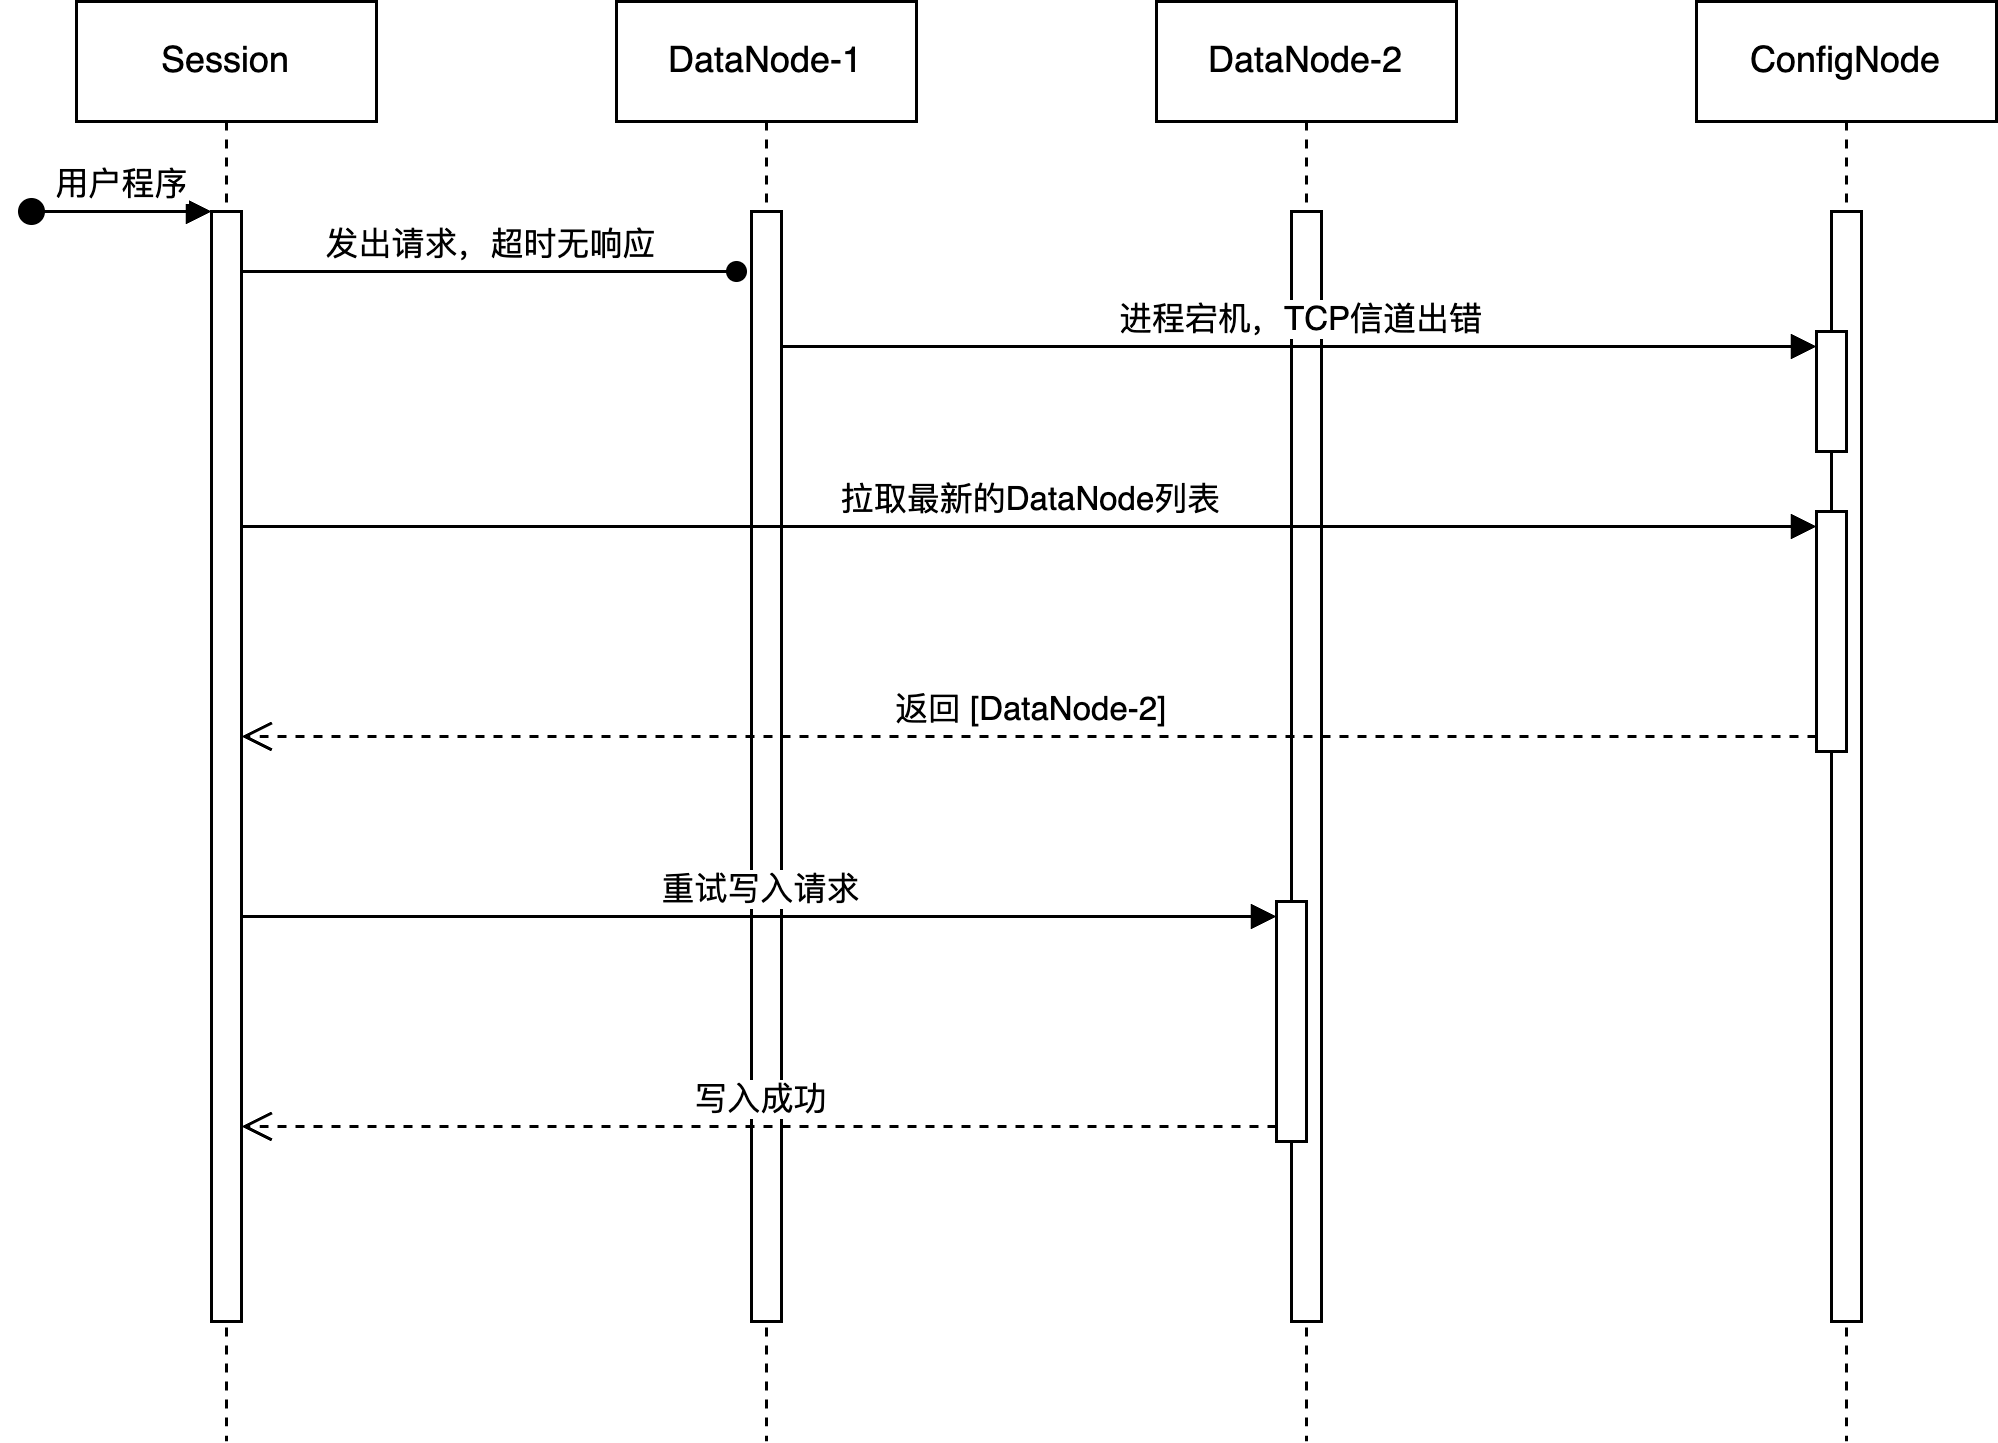
\includegraphics[width=0.99\linewidth]{c05-process-down-1.png}
    \caption{单节点进程宕机的高可用容错时序图}
    \label{fig:c05-process-down-1}
\end{figure}

图\ref{fig:c05-process-down-1}展示了高可用容错方案对于因DataNode宕机导致的用户连接直接失效的解决方案。图中DataNode1在处理Session的请求的时候出现了宕机,会导致Session的该请求超时无响应。
DataNode1宕机之后,ConfigNode可以通过心跳的方式检测出DataNode1的异常,并且更新该节点的状态。后续,由于Session具备后台进程会持续地从ConfigNode拉取最新的DataNode列表,因此最新一次的拉取将给出只有DataNode2存活的事实。
此时,Session会尝试重新向DataNode2发送请求。由于此时DataNode2正常工作,因此本次请求能够被正常处理,从而使用户的请求最终能够正常写入。


对于别的Coordinator连接到该DataNode上的请求,则会通过跟\ref{fig:c05-diskfull}相同的流程图来对其他的数据副本进行重试。

\section{对称网络分区}

\subsection{检测方法}
当DataNode节点和其他的节点出现了对称网络分区的情况下,由于节点依旧存活,所以不会因为关闭TCP信道的原因被发现。
此时,则需要通过上述的Phi Accural算法对节点的网络分区进行识别。具体来说,由于发给该节点的心跳都没有反应,在超过一定的时间之后,Phi Accrual算法就会判断该节点不可达,从而依然将节点的状态设置成UNKNWON

\subsection{高可用容错方案}

对于因为网络分区而失败的请求,则会通过跟\ref{fig:c05-diskfull}相同的流程图来对其他的数据副本进行重试。

\section{非对称网络分区}

\subsection{检测方法}
当DataNode节点和其他的DataNode节点出现了非对称网络分区的情况下,由于和ConfigNode之间的心跳通道能够正常交换心跳包,因此不会被ConfigNode的心跳机制所检测到。此时,则需要通过前文描述的拓扑感知的方式来进行判断。ConfigNode Leader会要求所有的DataNode定期测试和其他的所有DataNode的内部服务端口的连通性,并且上报每次的连通性的测试结果。
ConfigNode使用Phi Accural的检测算法对联通心跳进行检测,并实时判断。

\subsection{高可用容错方案}

\begin{figure}
    \centering
    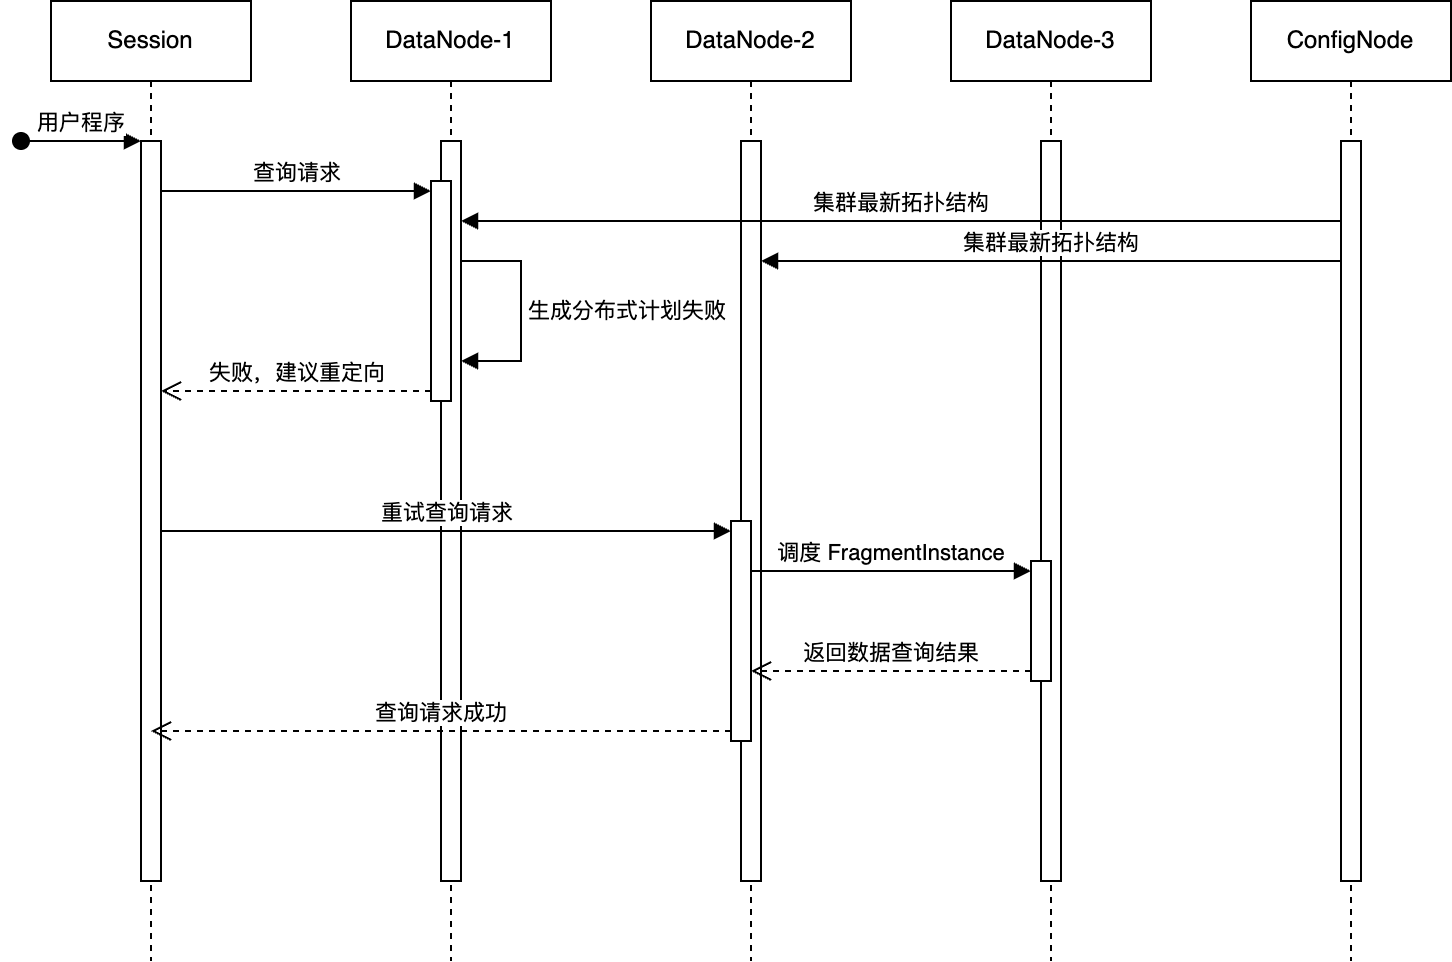
\includegraphics[width=0.99\linewidth]{c05-partition-asym.png}
    \caption{非对称网络分区的高可用容错时序图}
    \label{fig:c05-partition-asym}
\end{figure}

在非对称网络分区的情况下,需要Session和Coordinator两侧的协同才能解决这一类的问题。

图\ref{fig:c05-partition-asym}给出了非对称网络分区的高可用容错时序图。假设集群DataNode1和DataNode3之间出现了非对称网络分区。客户端连接到了DataNode-1上,并发送了查询请求。DataNode1在解析了查询请求之后,根据ConfigNode下发的最新集群拓扑,发现root fragment instance必须调度到DataNode3上,但是由于非对称网络分区的存在,该调度无法实现,因此DataNode1会返回失败的状态码,并附带重定向该请求的建议。

Session侧在获得重定向的失败消息之后,会尝试将该请求重定向到DataNode2上执行。由于DataNode2并不存在网络分区,能够和集群内的所有节点连接,因此查询规划能够顺利生成和调度,在多个DataNode之间进行数据的实际查询,完成本次的查询请求,将结果返回给Session的客户。

\section{ConfigNode节点脑裂}

ConfigNode是集群的大脑,负责管理集群的节点基础信息、现在的状态、集群的拓扑网络结构、集群的分区信息等,并且ConfigNode上运行着诸多后台的服务,包括负载均衡、Region迁移等服务。
我们需要保证ConfigNode服务的高可用,因此我们会运行多个ConfigNode的副本,每一个副本都保持了相同的数据,但是同一时刻只能有一个主副本发号施令,决定服务的实际状态。当主副本所在的ConfigNode节点出现宕机的时候,其他的副本则会通过选举流程产生一个新的主副本,接替相关的任务。

这种机制可能会出现脑裂的情况。具体来说,如果主副本短暂地发生了网络分区的情况,其他副本如果此时发起选举并且被正式选举为主副本,此时旧的主副本的网络分区恢复,且旧的主副本还没有意识到自己已经不再是Leader的情况下,就会导致集群中有两个主副本同时发号施令,从而出现所谓的脑裂情况。


我们通过设置Leader Lease和选举最小超时时间的方式来避免脑裂的结果。具体来说,如果Leader在一段时间没有收到来自大多数节点的心跳,那么Leader此时就会自己主动结束Leader的身份。而新的节点的最小选举超时需要大于Lease的时间。

这样做的好处在于能够保证集群的脑裂情况不会出现,但是坏处在于集群可能有一小段的时间ConfigNode的服务无法提供。此时,Session和Coordinator上请求ConfigNode节点的服务需要进行等待重试,防止出现这样的情况。

\begin{figure}
    \centering
    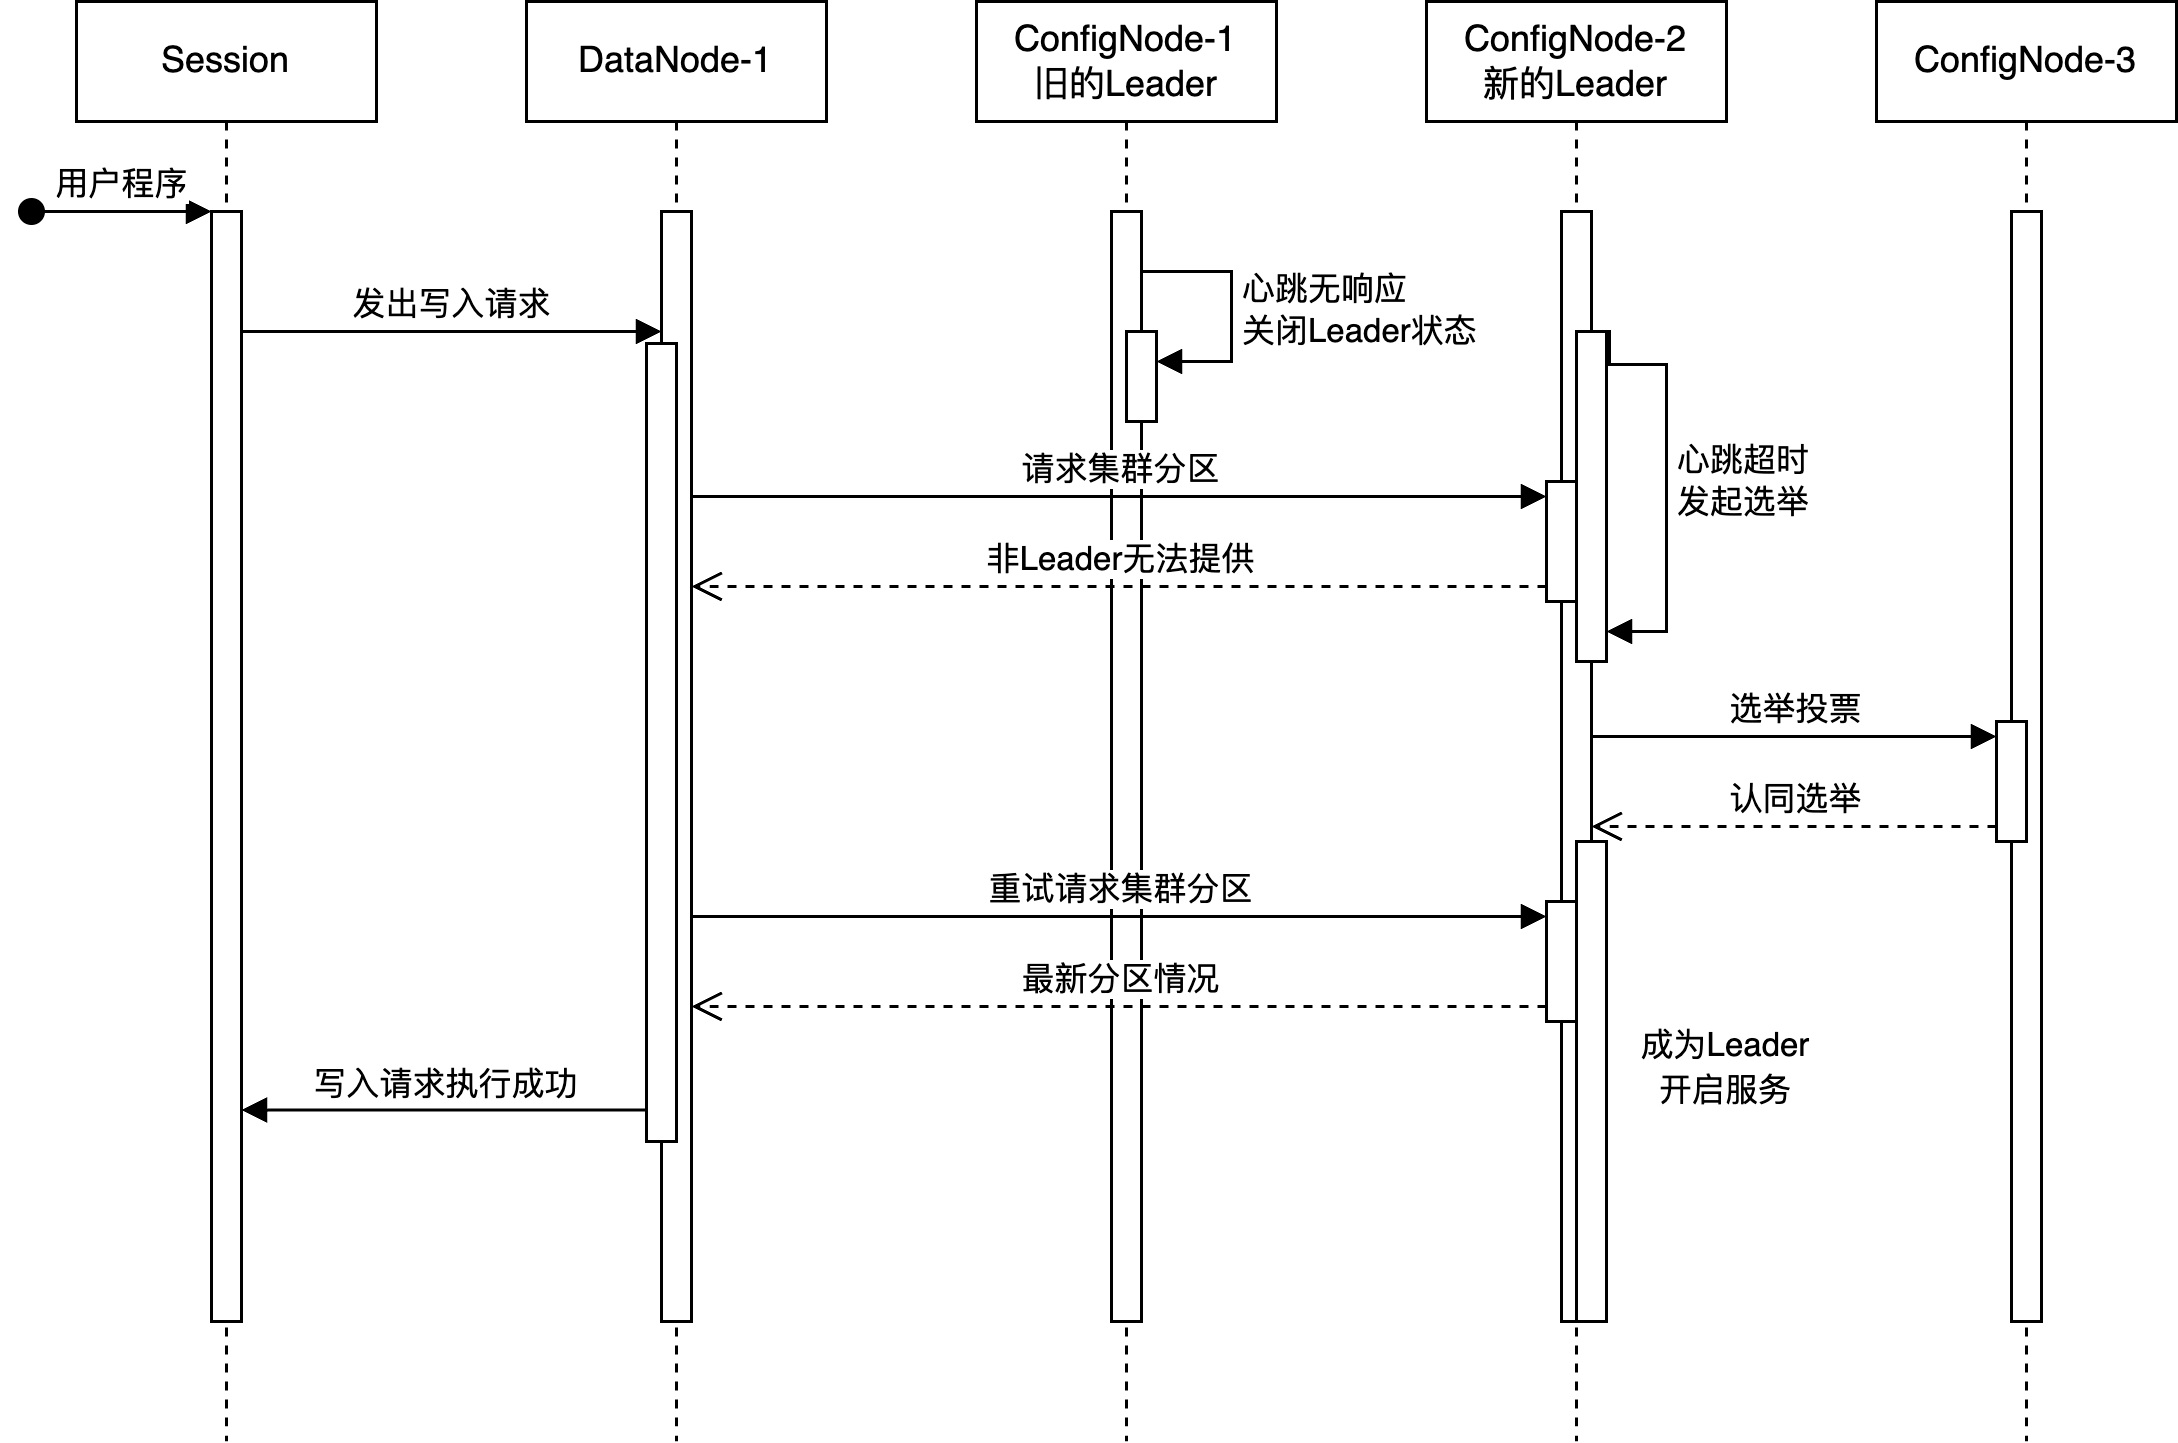
\includegraphics[width=0.99\linewidth]{c05-brain-split.png}
    \caption{ConfigNode服务的高可用容错时序图}
    \label{fig:c05-brain-split}
\end{figure}

图\ref{fig:c05-brain-split}展现了ConfigNode因为短暂的网络分区而导致服务不可用的情况下的高可用时序图。其中,ConfigNode-1是旧的Leader,由于和剩下的两个副本ConfigNode-2/ConfigNode-3之间出现了网络分区,导致在一段时间心跳无响应的状态下主动结束了Leader的服务。此时集群中没有ConfigNode节点能够提供服务。

此时,如果用户的写入和查询请求需要向ConfigNode获取分区等服务,那么这些请求就不能得到响应。此时,DataNode2需要等待一段时间,再进行重试。

在等待的这段时间里,ConfigNode-2率先出现选举超时,开始新一轮的选举,并在ConfigNode3的支持下成功当选最新一期的Leader,并正常开启了ConfigNode 的服务。此时,DataNode2再重试请求分区,ConfigNode2能够正常对其提供服务,DataNode也能够顺利完成请求的执行。

\section{集群变更状态下的一致性}

\subsection{错误检测}

在分布式IoTDB中,集群变更操作如Region迁移、节点扩缩容是保持集群拓展能力、负载均衡能力的必要手段。然而,这些操作在执行过程中不可避免地会引入短暂的数据不一致性,这种一致性可能会导致用户数据写入失败。

严格来讲,这种短暂的不一致性并非系统设计上的错误,也并非在系统运行中出现的故障,而是系统在追求极致可用性目标时所做出的权衡。

根据CAP原理\cite{fox1999harvest},在一个分布式系统中,一致性(Consistency)和可用性(Availability)往往难以同时保证。具体而言,如果系统在集群变更期间必须严格维护数据的绝对一致性,则必须暂停所有用户的写入操作,直至变更完成。这种做法虽然能够确保数据的一致性,但却极大地牺牲了系统的可用性,导致用户在一段时间内无法正常访问或操作数据。

IoTDB在设计的时候,选择在保证最终一致性的前提下,允许短暂的数据不一致性。因此,用户的请求可以随时到达,即使集群正处在变更的过程中,也会通过上述所言的三级重试来最大化地满足用户的请求。

\subsection{高可用容错方案}

\begin{figure}
    \centering
    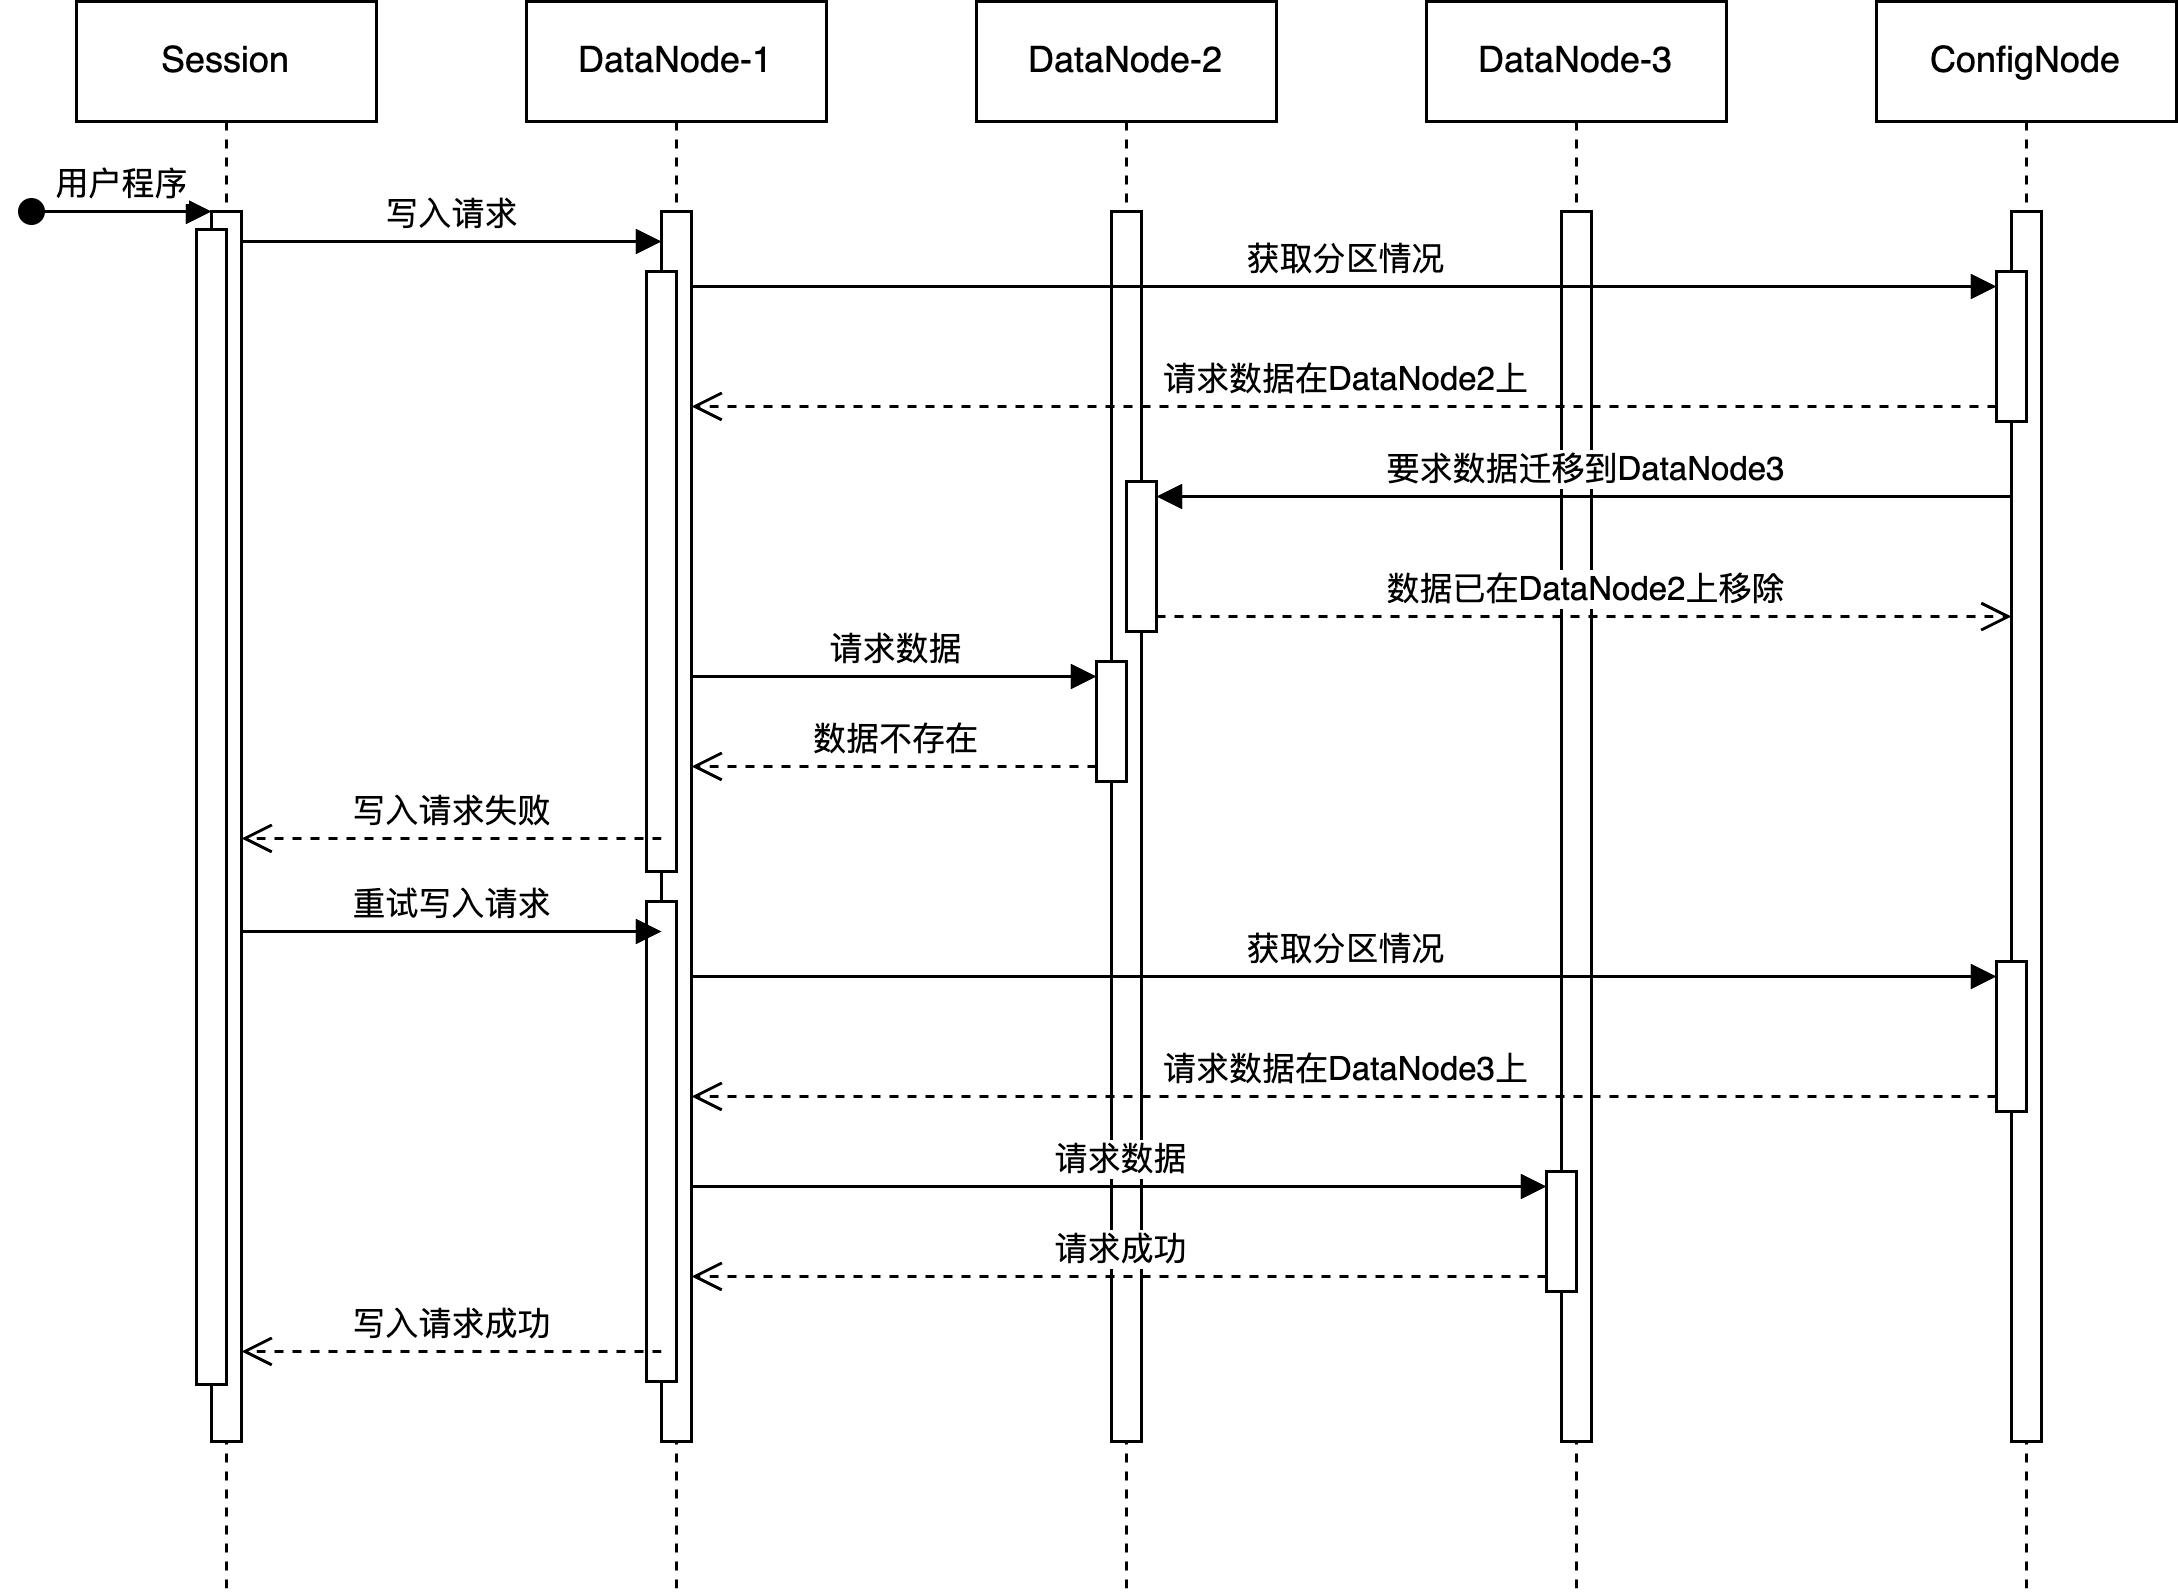
\includegraphics[width=0.99\linewidth]{c05-cluster-change.png}
    \caption{集群变更状态下高可用容错时序图}
    \label{fig:c05-cluster-change}
\end{figure}

图\ref{fig:c05-cluster-change}展示了在集群变更状态下系统的高可用容错时序图。用户在通过Session进行写入请求的时候,DataNode1先从ConfigNode这里获取了分区情况,并根据这个分区情况进行写入规划。然而,在规划期间,出于负载均衡的考虑,ConfigNode决定进行Region迁移的操作,将原本在DataNode2上的数据分区给迁移到DataNode3上。
写入规划对这一次Region迁移并不知情,并且继续向DataNode2发出请求,此时由于数据已被迁移出该节点,所以这个请求会以数据不存在的原因失败。
DataNode1会将这个情况返回给Session,并且附上重试的建议。Session会继续重试写入这个请求,这个请求会再次被发送到DataNode1上。此时,DataNode1会再次从ConfigNode这边获取最新的分区情况。此时最新的分区已经能够反映上次迁移的改变,因此DataNode1能够正确认识到数据此时存活在DataNode3上,从而向DataNode3发起请求,最终成功获取数据,本次写入也能顺利执行。
% !TeX root = ../thuthesis-example.tex

\chapter{实验章节}

本章将对前文所提出的高可用和容错能力进行实验,验证这些设计的效果。本章首先介绍实验环境,然后验证故障检测和判断能力,包括Phi Accrual研判算法的特性、和固定超时研判的比较、非对称网络分区和进程宕机场景下的检测能力。
然后再验证共识模块的三种协议在可用性上的表现,包括故障转移的速度、故障期间的性能和恢复的速度。
最后,本章节将会验证在进程宕机、磁盘写满、网络分区、集群变更等常见故障场景下的RTO和RPO数据。


\section{实验环境}


\begin{table}[h!]
    \centering
    \caption{服务器 环境}
    \label{tab:server_environment}
    \begin{tabular}{ll}
        \toprule
        配置 名称 & 配置 描述 \\
        \midrule
        CPU & Intel ( R ) Core ( TM ) i7-10700 CPU @ 2.90GHz 8 核 16 线程 \\
        内存 & 32GB \\
        磁盘 & 10TB HDD ( Seagate ST10000NM001G - 2MW103 ) \\
        网络 & 千兆 网卡 ( 1000Mb / s ) \\
        操作系统 & Ubuntu 20.04.5 LTS \\
        Java 版本 & OpenJDK 11.0.32 \\
        DataNode运行内存 & 28GB \\
        ConfigNode运行内存 & 2GB \\
        \bottomrule
    \end{tabular}
\end{table}

表格\ref{tab:server_environment}展示了测试所用的硬件环境和软件环境。测试机器分为4台,配置均为表格中展示的一致,三台用于运行IoTDB DataNode,一台用于运行IoTDB ConfigNode和测试程序。DataNode
分配了 28 GB 的内存,ConfigNode 分配了 2 GB 的内存。IoTDB 使用了一块希捷
ST-16000NM000J 机械硬盘作为存储设备,系统数据、写前日志、系统运行日志等
都会存储在同一块磁盘上。 IoTDB 使用了 OpenJDK 11.0.22 作为运行环境,操作系
统为 Ubuntu 20.04.2 LTS,64 位。测试机器之间的网络通过 1000 Mbps 的局域网连
接。

本文使用IoT-Benchmark\cite{iot-benchmark}模拟用户的写入负载。如无特殊说明,本章节所有实验所使用的IoT-Benchmark的配置如表格\ref{tab:iot-benchmark-default}所示。

\begin{table}[h!]
    \centering
    \caption{本章节测试所用IoT Benchmark配置}
    \label{tab:iot-benchmark-default}
    \begin{tabular}{ll}
        \toprule
        配置 名称 & 配置值 \\
        \midrule
        设备 数 & 100000  \\
        每个设备的序列数 & 10   \\
        存储组数 & 5  \\
        写入客户端数 & 25  \\
        每个写入请求的设备数 & 1000  \\
        每个写入请求中每个设备的记录数 & 1 \\
        \bottomrule
    \end{tabular}
\end{table}


\section{非对称网络分区故障的检测能力}

在本小节中,我们检测了IoTDB对于非对称网络分区的检测能力。

测试方法如下:设置IoTDB的Phi Accrual故障阈值为30,DataNode之间的对等心跳频率为5s一次,在节点平稳运行后的120s之后,使用防火墙iptables的命令阻断其中两个DataNode所在的通信,模拟非对称网络分区的故障,计时记录ConfigNode Leader研判集群出现非对称网络分区的速度。使用自动化工具重复上述过程1000次。

\begin{figure}
    \centering
    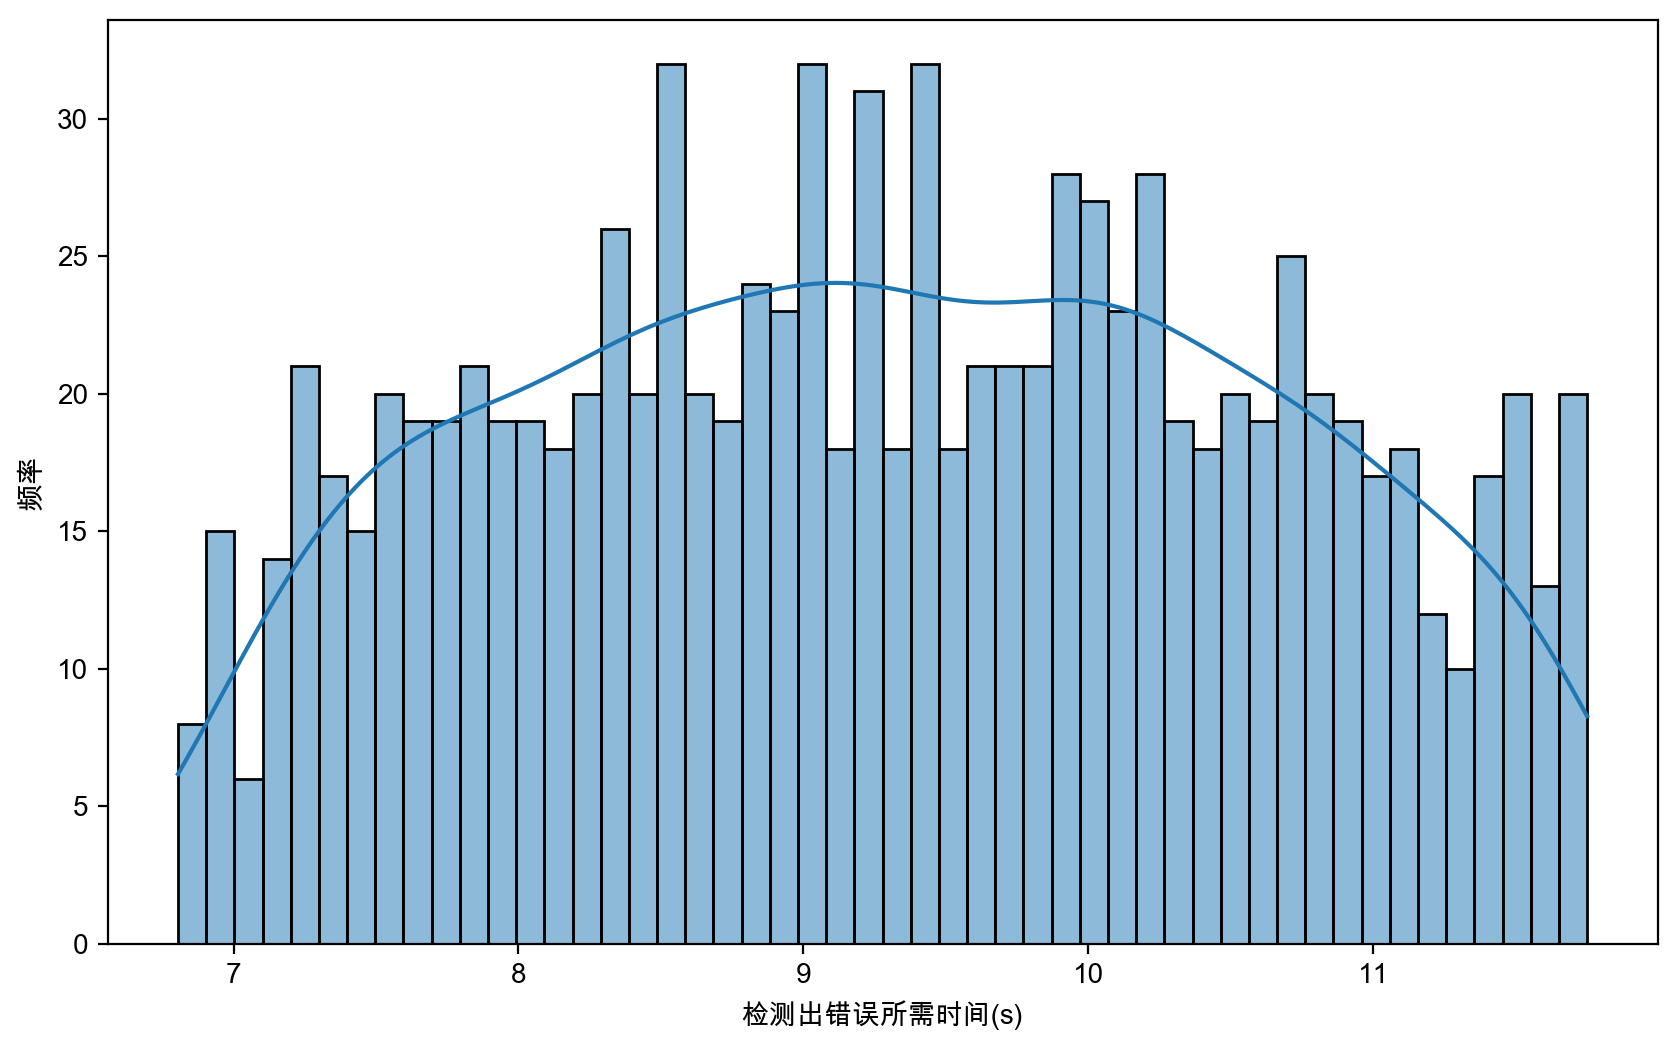
\includegraphics[width=0.8\linewidth]{exp-asym-np-detect.png}
    \caption{非对称网络分区检测故障所需时间的分布}
    \label{fig:exp-asym-np-detect}
\end{figure}

图\ref{fig:exp-asym-np-detect}展示了1000次实验中非对称网络分区检测所需时间的分布。1000次实验中,ConfigNode Leader无一例外全部检测到了非对称网络分区,平均的检测用时是9.30s,检测用时的标准差是2.08s。

\begin{figure}
    \centering
    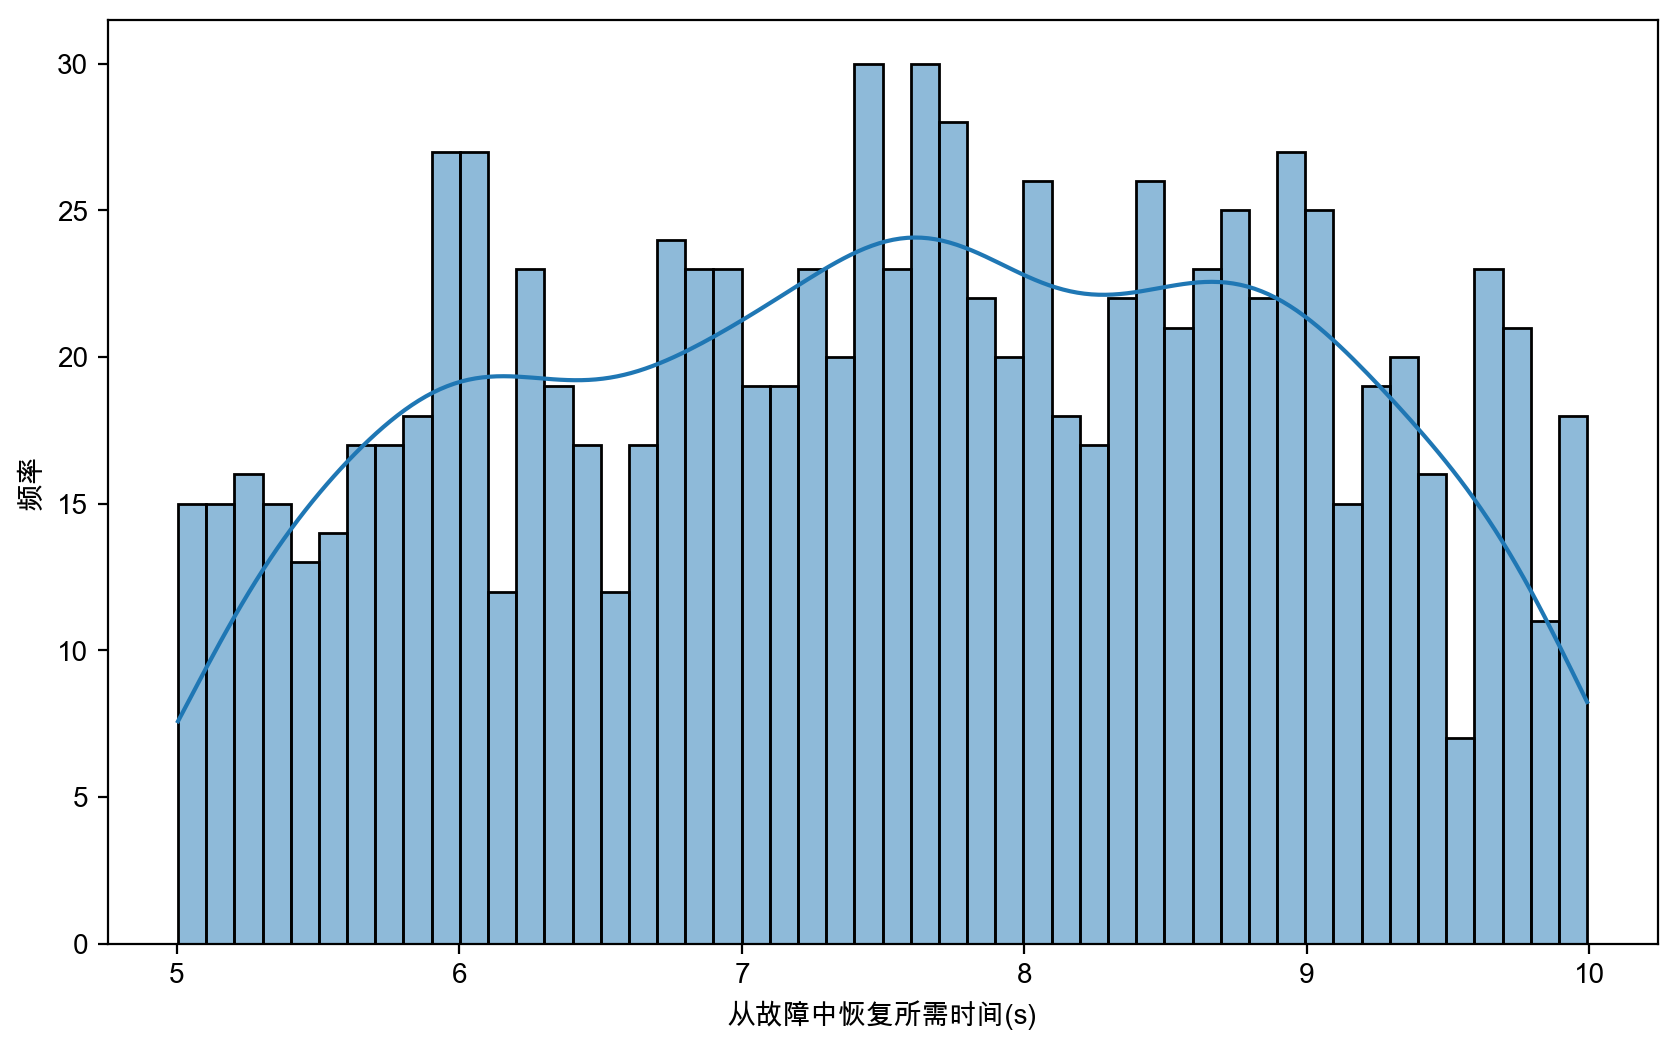
\includegraphics[width=0.8\linewidth]{exp-asym-np-recover.png}
    \caption{非对称网络分区检测恢复所需时间的分布}
    \label{fig:exp-asym-np-recover}
\end{figure}

在检测到非对称网络分区的120s后,解除防火墙的阻断,计时记录ConfigNode Leader研判集群不再具有非对称网络分区故障的时间。图\ref{fig:exp-asym-np-recover}展示了1000次实验中检测出非对称网络分区问题已恢复所需时间的分布。1000次实验中,ConfigNode Leader无一例外全部检测到了系统从非对称网络分区的故障中恢复,平均的检测用时为7.55s,检测用时的标准差是2.45s。

实验结果表明,IoTDB集群通过DataNode之间的对等心跳机制能够有效对非对称网络分区问题进行检测,且检测所需的时间在几秒到几十秒的范围内。当非对称网络分区结束后,心跳一经联通,IoTDB也会立即研判非对称网络分区问题结束。


\section{Phi Accrual故障研判算法的行为表现}

\subsection{算法的参数行为}

本文前面章节提出的基于Phi Accrual算法的故障检测机制具有两个可指定参数。
参数一是预设的故障检测阈值,默认为30。Phi Accrual算法会通过心跳的达到间隔采样窗口,计算节点的可能故障概率的指数量化指标Phi,并跟预设的故障检测阈值进行比较,给出故障研判的结果。
参数二是可容忍的最大心跳暂停,默认为10s。在JVM环境中,由于垃圾回收的机制可能导致进程暂停,因此对应的心跳也会暂停。为了容忍这种暂停,避免其影响研判的正确率,Phi Accrual允许设置最大的暂停时间。

本节给出了Phi Accrual在不同的参数下的行为表现。

\begin{figure}
    \centering
    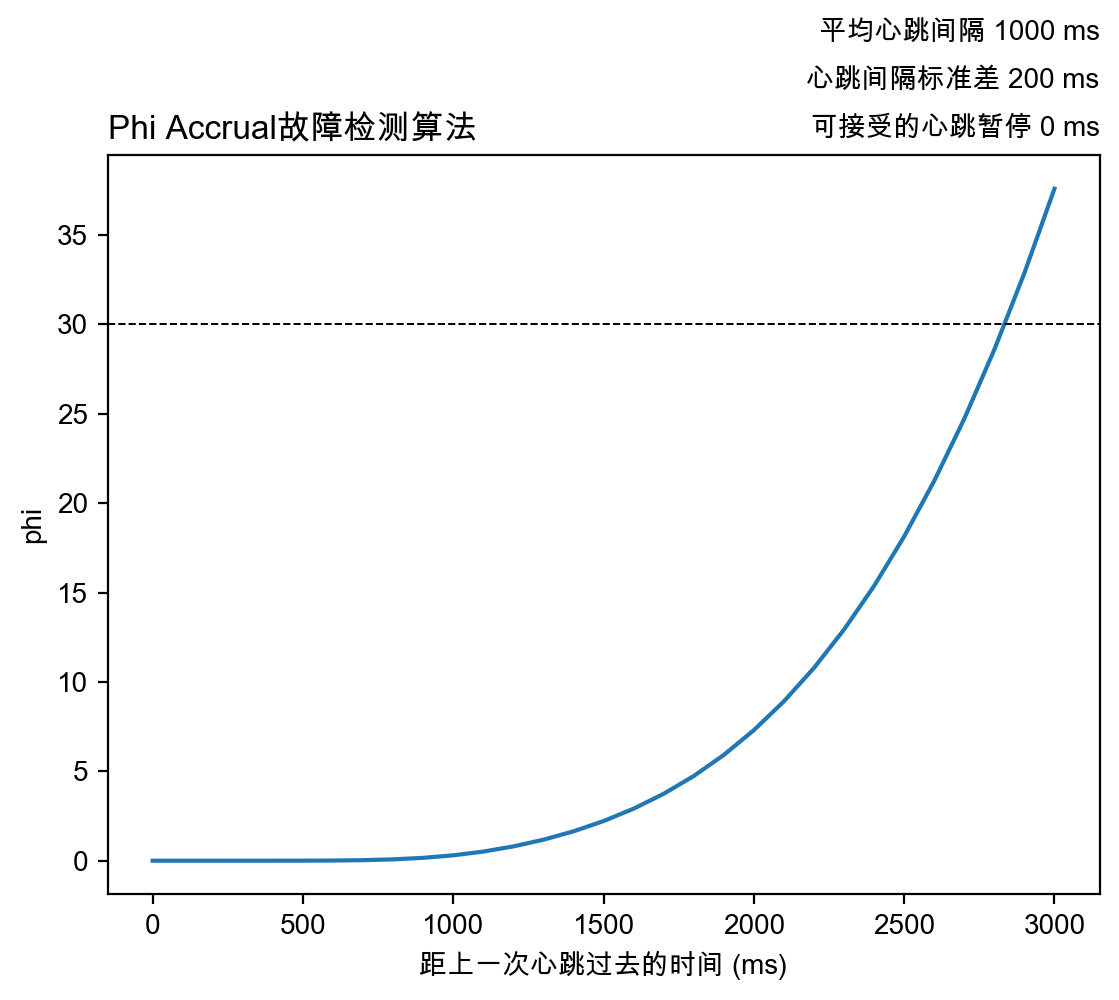
\includegraphics[width=0.6\linewidth]{exp-phi.png}
    \caption{Phi值随上一次心跳时间间隔变化示意图}
    \label{fig:exp-phi}
\end{figure}

图\ref{fig:exp-phi}展示了算法的故障概率量化指标Phi随着最后一次心跳经过的时间的变化情况。
在本次测试中,平均心跳之间的到达间隔约为1000ms,到达间隔的标准差固定为200ms,可容忍的最大心跳暂停为0。

实验结果表明了Phi Accrual算法能够在心跳长期未到达之后迅速给出故障预警。在距离最后一次心跳经过的时间范围不超过1000ms的时候,Phi值极低,接近零,代表此时算法研判的故障概率很低。超过1000ms之后,Phi值会随着最后一次心跳经过的时间呈指数型迅速升高,并在约2700ms的时候达到IoTDB的预设阈值30。这意味着如果2700ms没有接收到该有的心跳,Phi Accrual故障检测算法就会研判该节点出现了故障,这种检测效率远远高于原先的20s固定心跳超时。


\begin{figure}
    \centering
    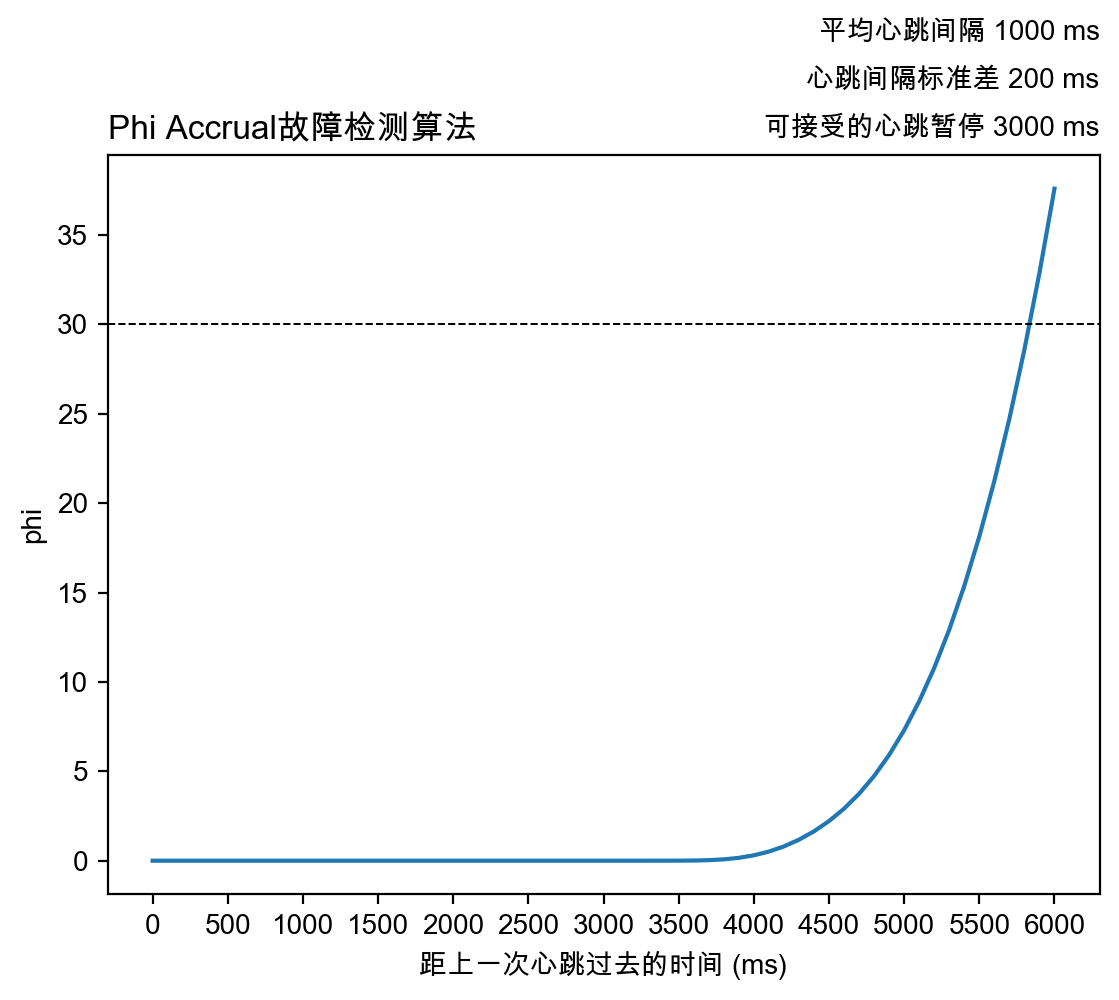
\includegraphics[width=0.6\linewidth]{exp-phi-with-pause.png}
    \caption{Phi值随上一次心跳时间间隔变化(带心跳暂停)示意图}
    \label{fig:exp-phi-with-pause}
\end{figure}

图\ref{fig:exp-phi}展示了可容忍的最大心跳暂停时间对于故障研判的影响。。
在本次测试中,平均心跳之间的到达间隔约为1000ms,到达间隔的标准差固定为200ms,可容忍的最大心跳暂停为3000ms。

实验结果表明了,Phi Accrual算法能够较好地容忍JVM垃圾回收造成的进程暂停等情况。可容忍的最大心跳暂停时间这一参数能够线性地影响Phi值的计算。在距离最后一次心跳经过的时间范围不超过4000ms的时候,Phi值极低,接近零,代表此时算法研判的故障概率很低。超过4000ms之后,Phi值会随着最后一次心跳经过的时间呈指数型迅速升高,并在约6700ms的时候达到IoTDB的预设阈值30。相较于上一组实验,每一个关键节点都朝右偏移了3000ms,表明了Phi值计算受可容忍的最大心跳暂停时间线性影响的特点。


\subsection{Phi Accrual和固定超时算法在不同场景下的检测能力}
本小节比较了基于Phi Accrual的故障检测算法和基于固定超时的故障检测算法在现实场景中的故障检测能力。场景包括正常运行场景、高负载场景、负载呈周期性变化场景、负载逐渐升高场景,故障检测能力的指标是平均故障发现时间和平均的误报次数。

本节的测试通过使用用户负载模拟程序IoT Benchmark实现,不同场景的Benchmark的配置参数如表\ref{tab:extended_columns}所示,表格中的t代表运行的时间,单位是分钟。

\begin{table}[h!]
    \centering
    \caption{不同负载场景的IoT Benchmark配置}
    \label{tab:extended_columns}
    \begin{tabular}{lllll}
        \toprule
        配置 名称 & 正常负载 & 高负载 & 周期负载 & 负载逐渐升高 \\
        \midrule
        设备 数 & 100000 & 100000 & 100000 & 100000 \\
        每个设备的序列数 & 10 & 10 & 10 & 10  \\
        存储组数 & 5 & 5 & 5 & 5 \\
        写入客户端数 & 25 & 25 & 25 & 25 \\
        每个写入请求的设备数 & 1000 & 1000 & 1000 & 1000 \\
        每个写入请求中每个设备的记录数 & 1 & 10 & 1 + 20*(t mod 2) & 1 + max(t/20,20) \\
        \bottomrule
    \end{tabular}
\end{table}

本节测试的参数选择:ConfigNode和DataNode之间交换心跳的间隔为1s,固定心跳超时被设置在20s,Phi Accrual的超时阈值在30,可容忍的最大心跳暂停为10s。

\begin{table}[h!]
    \centering
    \caption{正常运行场景下的固定超时和Phi Accrual算法对比}
    \label{tab:exp-normal-load}
    \begin{tabular}{@{}llll@{}}
        \toprule
        场景 & 算法 & 平均故障发现延迟 (s) & 平均误报次数(100次中) \\
        \midrule
        正常运行 & 固定心跳超时 & \SI{20.02}{\second} & 0 \\
        正常运行 & Phi Accrual & \SI{13.85}{\second} & 0 \\
        \bottomrule
    \end{tabular}
\end{table}

表\ref{tab:exp-normal-load}给出了正常运行场景下固定超时算法和Phi Accrual算法的对比。
实验方法如下:运行在持续运行120s之后,按照50\%的概率杀死一个进程,接着记录两个算法发现故障的平均延迟和误报情况。在本场景下GC暂停的时间通常不超过1s。
实验结果表明了,在正常运行期间,Phi Accrual相较于固定心跳超时能够更快地检测出错误,两者在不受GC暂停的影响下误报率都非常的低。


\begin{table}[h!]
    \centering
    \caption{高负载运行场景下的固定超时和Phi Accrual算法对比}
    \label{tab:exp-high-load}
    \begin{tabular}{@{}llll@{}}
        \toprule
        场景 & 算法 & 平均故障发现延迟 (s) & 平均误报次数(100次中) \\
        \midrule
        高负载运行 & 固定心跳超时 & \SI{20.09}{\second} & 5 \\
        高负载运行 & Phi Accrual & \SI{22.80}{\second} & 1 \\
        \bottomrule
    \end{tabular}
\end{table}

表\ref{tab:exp-high-load}给出了高负载运行场景下固定超时算法和Phi Accrual算法的对比。
实验方法如下:运行在持续运行120s之后,按照50\%的概率杀死一个进程,接着记录两个算法发现故障的平均延迟和误报情况。在本场景下GC暂停的总时间达到总CPU时间的20\%,单次GC暂停的时间从一秒到十几秒不等。
实验结果表明了,在高负载运行场景下,
Phi Accrual的检测速度略微低于固定心跳,但是误报率大大下降,达到了发现延迟和误报率的较好的一个平衡。如果GC暂停的时间远大于固定超时20s,那么固定心跳超时的误报率将会呈直线上升的趋势。


\begin{table}[h!]
    \centering
    \caption{负载逐渐提高场景下的固定超时和Phi Accrual算法对比}
    \label{tab:exp-increase-load}
    \begin{tabular}{@{}llll@{}}
        \toprule
        场景 & 算法 & 平均故障发现延迟 (s) & 平均误报次数(100次中) \\
        \midrule
        负载逐渐提高 & 固定心跳超时 & \SI{20.08}{\second} & 17 \\
        负载逐渐提高 & Phi Accrual & \SI{24.45}{\second} & 4 \\
        \bottomrule
    \end{tabular}
\end{table}

表\ref{tab:exp-increase-load}给出了负载逐渐提高运行场景下固定超时算法和Phi Accrual算法的对比。
实验方法如下:运行在持续运行120s之后,按照50\%的概率杀死一个进程,接着记录两个算法发现故障的平均延迟和误报情况。在本场景下GC暂停的总时间达到总CPU时间的27\%,单次GC暂停的时间从一秒到几十秒不等。随着测试时间的增加,GC暂停的频率和时长都有所增加。

实验结果表明了,在负载逐渐提高运行场景下,
Phi Accrual和固定心跳超时的误报率都有所上升,但Phi Accrual的误报率依然远低于固定心跳超时。两者的检测速度依然相似,Phi Accrual的故障发现延迟略微低于固定心跳。


\begin{table}[h!]
    \centering
    \caption{负载周期行变化场景下的固定超时和Phi Accrual算法对比}
    \label{tab:exp-seasonal-load}
    \begin{tabular}{@{}llll@{}}
        \toprule
        场景 & 算法 & 平均故障发现延迟 (s) & 平均误报次数(100次中) \\
        \midrule
        负载周期变化 & 固定心跳超时 & \SI{19.98}{\second} & 11 \\
        负载周期变化 & Phi Accrual & \SI{23.20}{\second} & 2 \\
        \bottomrule
    \end{tabular}
\end{table}

表\ref{tab:exp-high-load}给出了负载周期变化运行场景下固定超时算法和Phi Accrual算法的对比。
实验方法如下:运行在持续运行120s之后,按照50\%的概率杀死一个进程,接着记录两个算法发现故障的平均延迟和误报情况。在本场景下GC暂停的总时间达到总CPU时间的25\%,单次GC暂停的时间从一秒到几十秒不等,GC暂停的时间和频率能够观察到周期性变化,但略微落后于负载的周期性变化。

实验结果表明了,在负载周期变化场景下,
Phi Accrual依然保持了非常良好的动态调整能力,误报率依然保持在很低的水平。Phi Accrual的检测速度略微低于固定心跳,但实际差距并不明显。

总结来说,通过模拟四种不同负载的场景,我们能够得出以下结论:Phi Accrual算法在正常场景下有着更快的故障检测速度,并且展现出了出了随着系统实际负载变化而变化的自适应能力,在负载较高或者负载变化的场景下能够以牺牲微量检测时延的代价获得极低的误报率。


\subsection{基于Thrift连接的进程宕机检测速度}

\begin{table}[h!]
    \centering
    \caption{进程宕机情况下故障发现优化实验}
    \label{tab:exp-thrift-process-down}
    \begin{tabular}{@{}llll@{}}
        \toprule
        场景 & 算法 & 平均故障发现延迟 (s) \\
        \midrule
        进程宕机 & 基于心跳和研判算法 & \SI{13.72}{\second}  \\
        进程宕机 & 基于Thrift连接状态 & \SI{0.05}{\second}  \\
        \bottomrule
    \end{tabular}
\end{table}

表\ref{tab:exp-thrift-process-down}给出了基于Thrift连接的进程宕机故障发现的优化验证。保持故障检测算法Phi Accrual的默认参数检测阈值为30,ConfigNode和DataNode的心跳间隔为1s。

实验结果表明,基于Thrift连接状态的主动通知型故障检测的延迟显著低于基于心跳历史的研判算法。


\section{副本和共识协议}

\subsection{故障后的容错表现}

本小节测试了三种共识协议在副本发生故障之后的容错表现。测试方法如下:为每一个协议配置三个副本,使用三个IoT-Benchmark分别向三个副本写入,并在运行一段时间之后手动关闭一个副本,模拟副本故障的情况,并且保持写入,衡量前后的吞吐变化。Session在发现故障后重试的配置参数为3次,每次需要等待1s才会执行。RatisConsensus的副本选举时间设定为4s到8s之间。

\begin{figure}
    \centering
    \includegraphics[width=0.99\linewidth]{exp-consensus-failure.png}
    \caption{不同共识协议的故障容错表现}
    \label{fig:exp-consensus-failure}
\end{figure}


图\ref{fig:exp-consensus-failure}展示了测试的结果。

在故障发生之后吞吐的下降峰值是衡量共识协议可用性的一个指标。如图所示,IoTConsensus在单一副本故障之后吞吐下降了33\%,IoTConsensusV2在单一副本故障之后吞吐下降了37\%,RatisConsensus在单一副本故障之后吞吐下降了96\%。
实验结果表明,IoTConsensus和IoTConsensusV2在单一副本故障发生时有着更好的可用性,因为其他不受影响的副本可以独立服务写入请求,使得总吞吐量大约下降1/3。但是RatisConsensus在单一副本(主副本)发生故障时有一段时间的不可用,原因是共识协议需要重新选举新的主副本,在新的主副本选举完成之前所有副本都无法接受写入请求。

在故障发生之后吞吐的恢复速度是衡量共识协议错误转移速度的一个指标。
当Session检测到节点故障之后,会通过DataNode发现和重定向的方式,将原来连接到故障节点的请求重定向到正常的节点上,从而完成写入的恢复。
如图所示,IoTConsensus和IoTConsensusV2在故障后约3-5s写入吞吐就能大致恢复,而RatisConsensus在故障后约8s写入吞吐才大致恢复。
由于重试和超时时间的设置,Session需要至少3s才会进行请求的重定向,这跟我们的实验结果比较吻合。RatisConsensus这边多出来的时间是Leader重新选举的选举超时。

实验结果表明,IoTConsensus和IoTConsensusV2有着更极致的可用能力,在单一副本发生故障的时候的吞吐下降峰值、吞吐恢复速度两个指标上都更优于RatisConsensus。



\subsection{故障副本的恢复时间}

本小节测试了在三种不同共识协议的故障副本恢复表现。测试方法如下:为每一个协议配置三副本,使用IoT-Benchmark持续写入数据。在写入数据5分钟之后,手动结束一个副本的进程,模拟故障的发生,但保持数据继续写入其他副本。再过五分钟之后,重启这个故障的副本,测试这个故障恢复的副本从进程重启到已经同步完宕机期间所有数据所需要的时间。IoTConsensusV2使用数据同步百分比代表追赶进度,IoTConsensus使用WAL的index代表追赶进度,而RatisConsensus使用Raft Term和Index代表追赶进度。

\begin{figure}
    \centering
    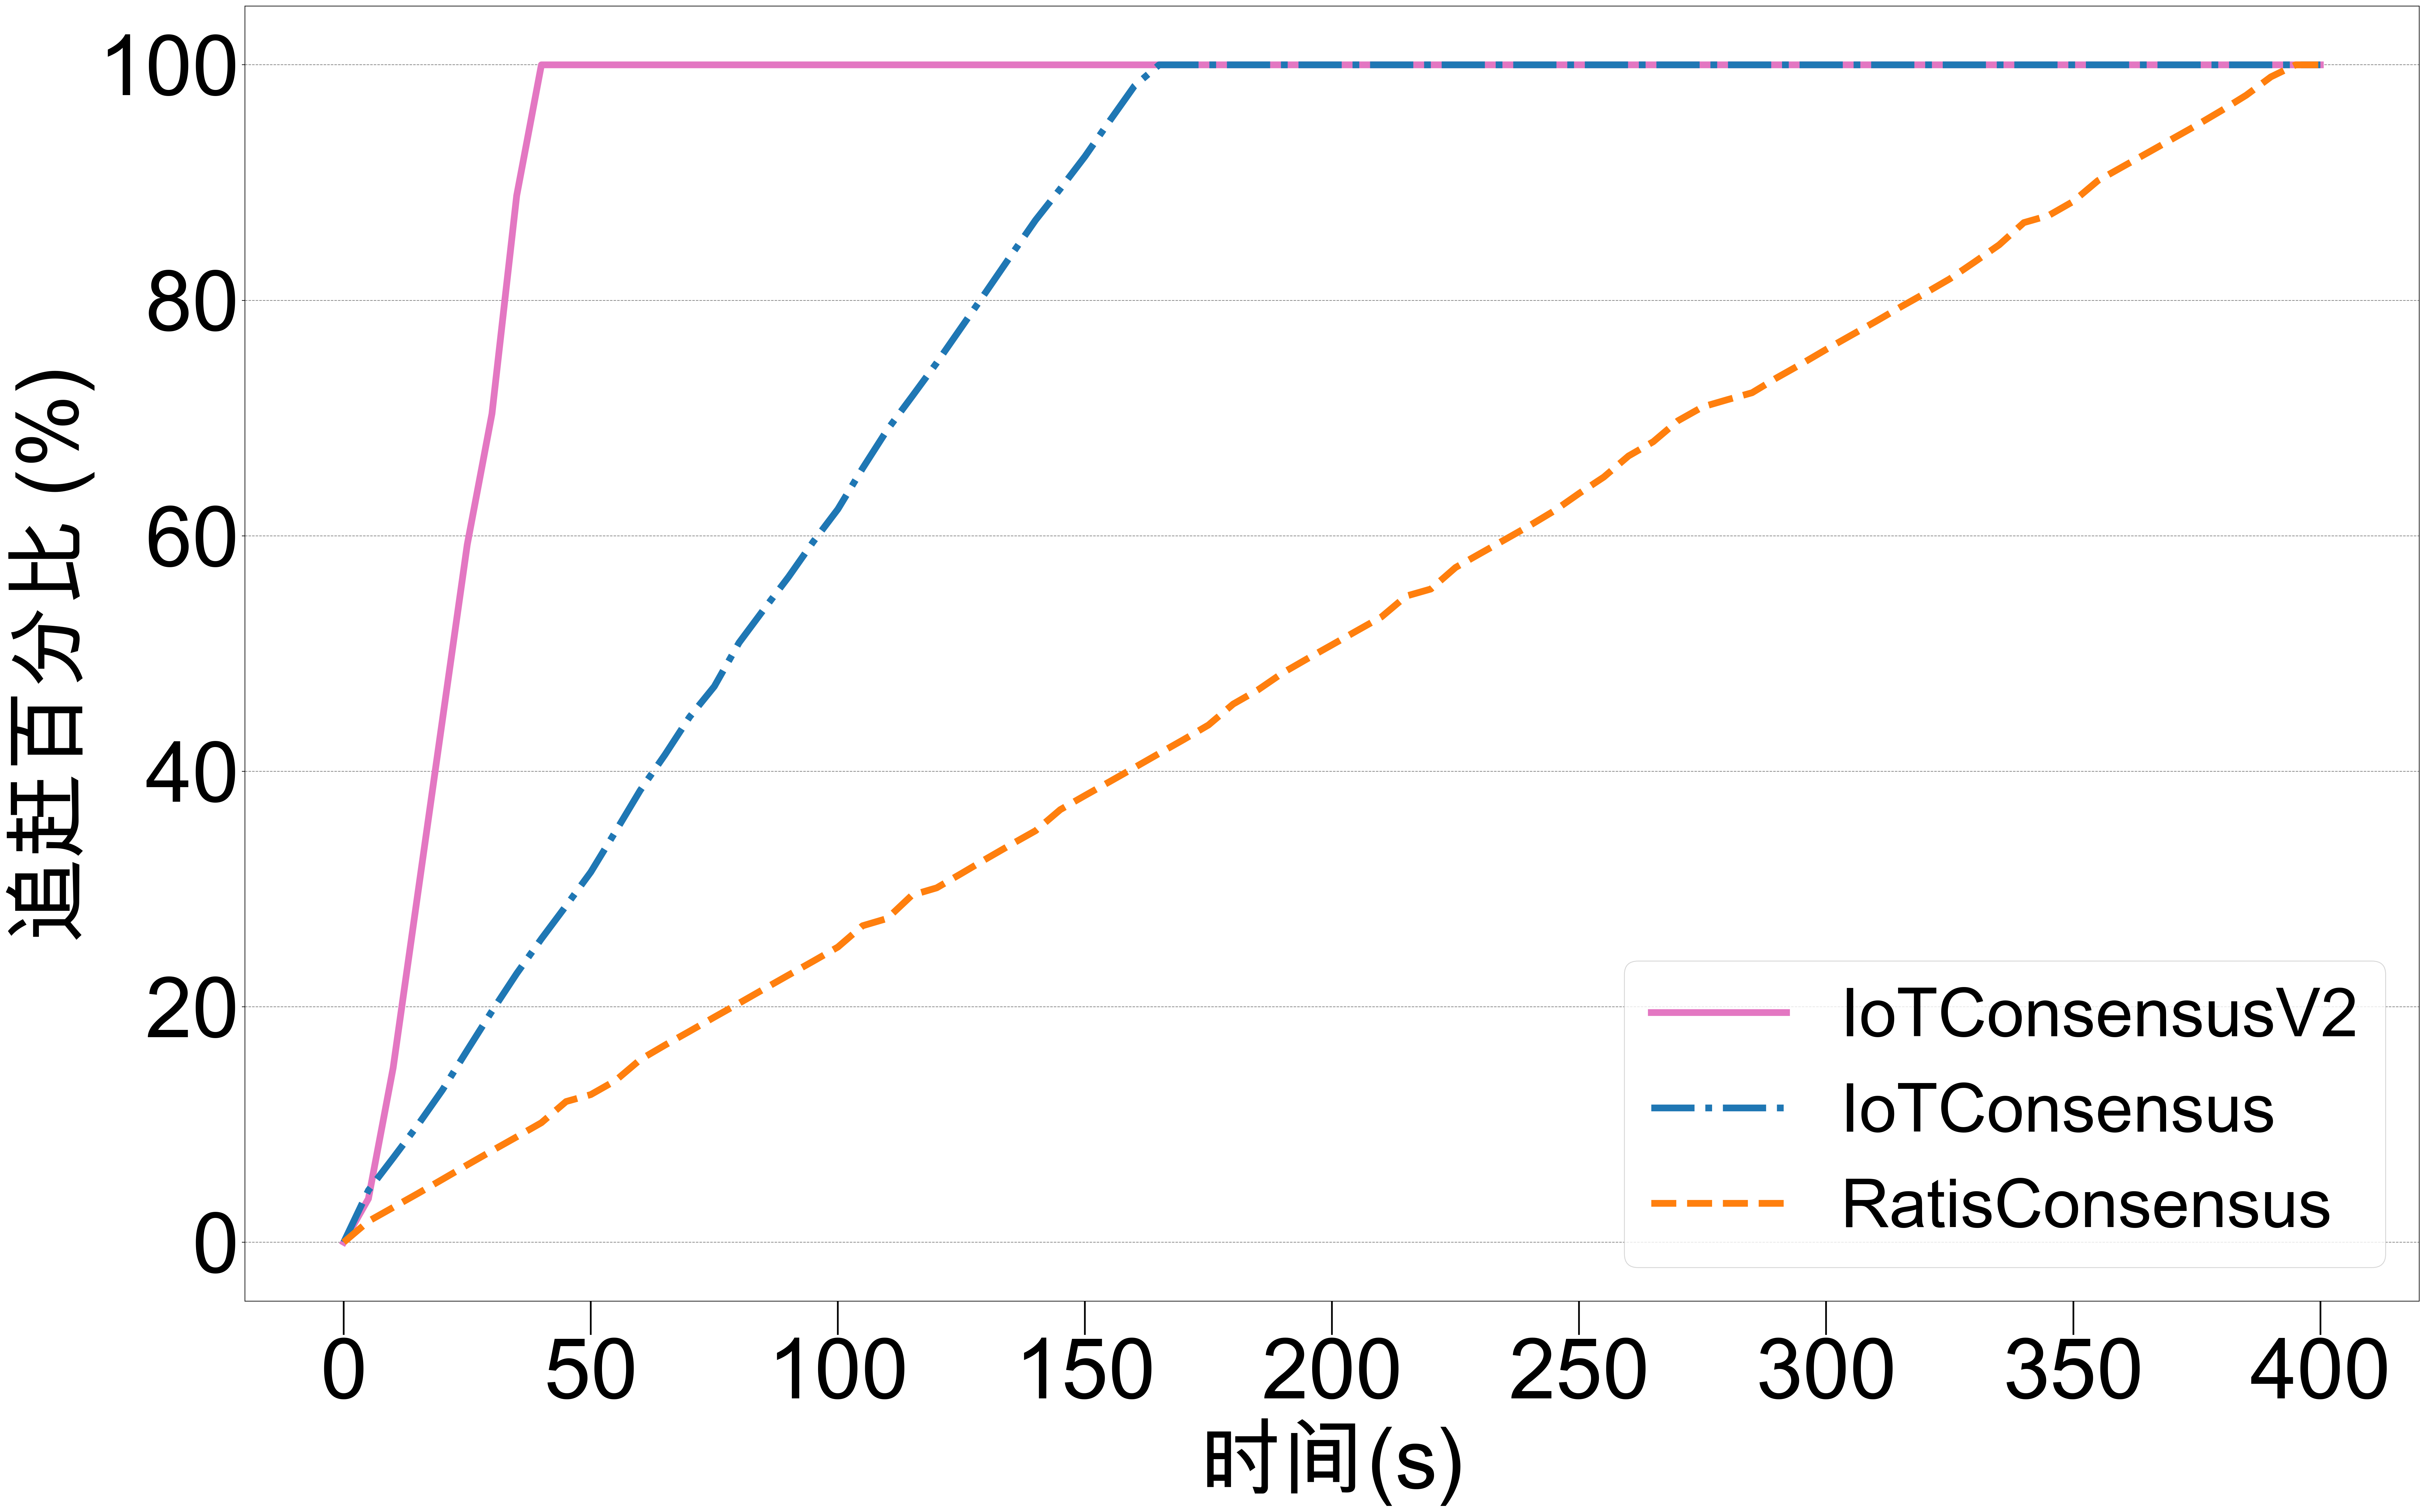
\includegraphics[width=0.8\linewidth]{exp-catch-up.png}
    \caption{不同共识协议的故障副本恢复表现}
    \label{fig:exp-catch-up}
\end{figure}

图\ref{fig:exp-catch-up}展示了实验的结果。在重启之后,IoTConsensusV2使用了40s的时间同步完了宕机期间的数据,IoTConsensus使用了170s的时间完成同步,而RatisConsensus使用了390s的时间完成同步。

实验结果表明,三种共识协议都能够自动恢复故障的副本。由于IoTConsensusV2通过TsFile进行数据传输,在恢复速度上显著优于IoTConsensus和RatisConsensus。


\section{故障场景的RTO和RPO情况}



本节测试了\ref{chap-failure-scenarios}章节中描述的常见错误场景的RTO和RPO情况。




端到端测试:

4. 不同故障场景不同的RTO情况
3个benchmark写入三个副本,

SR 统一用 Ratis,DataRegion 可以换 RatisConsensus, IoTConsensus, IoTConsensus

4.1 磁盘写满(用 readonly 就行)

IoT/IoTConsensusV2: 短暂下降1s左右,然后导引到其他节点,然后开始下降20\%
Ratis-Follower: 短暂下降1s左右,然后导引到其他节点,然后开始下降10p
Ratis-Leader:在6s内下降到0,然后引导到其他节点,然后开始下降10p



4.2 进程宕机(测试 kill -9 和脚本停止两种场景)
4.3 非对称网络分区(A,B,C 三个节点,其中两个节点之间无法通信)

IoTConsensu


4.4 对称网络分区(A,B,C 三个节点,其中 A 与其它两个节点无法通信)
4.5 集群变更(并发读写过程中测试缩容)




\section{和其他数据库的RTO和RPO对比}

% !TeX root = ../thuthesis-example.tex

\chapter{总结与展望}


\section{本文总结}


\section{本文不足与展望}


% 其他部分
\backmatter

% 参考文献
\bibliography{ref/refs}  % 参考文献使用 BibTeX 编译
% \printbibliography       % 参考文献使用 BibLaTeX 编译

% 致谢
% !TeX root = ../thuthesis-example.tex

\begin{acknowledgements}

时光荏苒,岁月如梭,历时三年的研究生生涯即将画上一个圆满的句号。
这是一段充满着挑战和收获的时光,一段美好和艰辛并存的时光。在清华园里,我丰收了专业知识和技能,学到了做人做事的道理,和师门同窗结下了一段深厚的友谊。回首过去飞速成长的三年,我心中充满了无限的感激。

这篇论文得以顺利完成,我要特别感谢我的指导老师,王建民教授。高山仰止,景行景止,王老师严谨的治学态度、深厚的学术造诣以及对科研工作的无限热情、对学生的亲切关爱,都让我深感动容。他不仅在学术上为我指明了方向,更在人生道路上给予了我很多启迪。没有王老师的悉心指导和严格要求,我不可能取得今天的成绩。

同时,我还要衷心感谢在我的学习和科研过程中给予我指导和帮助的黄向东老师和乔嘉林老师。
在论文的选题、开题、研究过程、数据分析到最终定稿的每一个环节,黄老师和乔老师都提供了宝贵的建议和支持。各位老师的教诲和帮助,使我受益匪浅,在此一并表示诚挚的谢意。

我的父母是我永远坚实的后盾。感谢他们一直以来无私的爱、默默的支持和辛勤的付出。是他们无条件的理解、鼓励和支持,帮我顺利地度过了困难时期,更加心无旁骛地投入到学习和科研中。这份沉甸甸的爱,是我前行的最大动力。

此外,我要感谢师门的学长学姐和学弟们。我们因共同的缘分连结,形成一个一个温暖的大家庭,在这里我们共同成长,留下了无数珍贵的回忆。我会一直记得那些宝贵经验的分享、无数次的夜聊、一同出游的美好。

感谢我的同窗陈荣钊、陈彦泽、廖兰宇、权思屹、伊丹翔、张洪胤和郭礼华,感谢我们一起度过的无数个奋斗的日夜,一起探讨问题,一起克服困难,一起欢声笑语。他们让我的研究生生活充满了阳光和温暖,也成为这段研究生生涯回忆中最闪耀的篇章。我们之间建立的深厚友谊将是我一生宝贵的财富,在这里祝福各位都能奔赴美好的前程。

最后,在这段独特的历史舞台上,感谢每一个曾闪耀过的人。你们都以各自独特的方式,在这段旅程中留下了或深或浅的印记。感谢你们出现在我的生命里,让这段攻读学位的时光充满了色彩和意义。

长风破浪会有时,直挂云帆济沧海。我将满怀坚定的热情,追求更卓越的成就,不辜负所有人的期望。

\end{acknowledgements}


% 声明
% 本科生开题报告不需要
\statement
% 将签字扫描后的声明文件 scan-statement.pdf 替换原始页面
% \statement[file=scan-statement.pdf]
% 本科生编译生成的声明页默认不加页脚,插入扫描版时再补上;
% 研究生编译生成时有页眉页脚,插入扫描版时不再重复。
% 也可以手动控制是否加页眉页脚
% \statement[page-style=empty]
% \statement[file=scan-statement.pdf, page-style=plain]

% 个人简历、在学期间完成的相关学术成果
% 本科生可以附个人简历,也可以不附个人简历
% !TeX root = ../thuthesis-example.tex

\begin{resume}

  \section*{个人简历}

  我是宋子阳


  % \section*{在学期间完成的相关学术成果}

  % \subsection*{学术论文}

  % \begin{achievements}
  % \end{achievements}


  % \subsection*{专利}

  % \begin{achievements}
  %  \end{achievements}

\end{resume}


% 指导教师/指导小组评语
% 本科生不需要
% !TeX root = ../thuthesis-example.tex

\begin{comments}
% \begin{comments}[name = {指导小组评语}]
% \begin{comments}[name = {Comments from Thesis Supervisor}]
% \begin{comments}[name = {Comments from Thesis Supervision Committee}]

宋子阳同学热爱党、热爱祖国,品行端正,政治表现好。

论文结构清晰,语句通顺,论述清晰。

论文工作表明该同学已经掌握软件工程学科坚实的基础理论和系统的专门知识,具有一定开展工程实践和科研工作的能力。

宋子阳同学学术作风严谨,同意组织其硕士学位论文答辩。
\end{comments}


% 答辩委员会决议书
% 本科生不需要
% !TeX root = ../thuthesis-example.tex

\begin{resolution}

\end{resolution}


% 本科生的综合论文训练记录表(扫描版)
% \record{file=scan-record.pdf}

\end{document}
